\documentclass[spanish]{book}
\usepackage[T1]{fontenc}
\usepackage[utf8]{inputenc}
\usepackage[spanish]{babel}
\usepackage{geometry}
\usepackage{tikz}
\usepackage{pgfplots}
\pgfplotsset{compat=1.18}
\usepackage{pdfpages}
\usepackage{listings}
\usepackage{color}
\usepackage{array}
\usepackage{graphicx}
\usepackage{setspace}
\usepackage{fancyhdr}
\usepackage[center,font=small,format=plain,labelfont=bf,up,textfont=it,up]{caption}
\usepackage{amsmath}
\usepackage{tocloft}  % Para crear el índice de ecuaciones
\usepackage{rotating}
\usepackage{float}
\usepackage{tabularx}
% Definir un color amarillo claro
\definecolor{codebg}{rgb}{1.0, 1.0, 0.8}

% Definir el estilo json para lstlisting
\lstdefinestyle{json} {
    backgroundcolor=\color{codebg},
    basicstyle=\ttfamily,
    language=json,
    stepnumber=1,
    numberstyle=\tiny,
    breaklines=true,
    captionpos=b,
    frame=single,
    frameround=tttt,
    rulecolor=\color{black}
}

% --- Configuración de márgenes ---
\geometry{
    verbose,
    tmargin=2.5cm,
    bmargin=2.5cm,
    lmargin=3cm, % Margen izquierdo en páginas impares
    rmargin=3cm  % Margen derecho en páginas pares
%bindingoffset=0cm,  % Ajusta este valor si tienes encuadernación
}



% --- Configura la sangría y el espacio entre párrafos ---
\setlength{\parindent}{0pt}  % Elimina la sangría de primera línea
\setlength{\parskip}{0.5em}  % Ajusta el espacio entre párrafos (ajusta el valor según sea necesario)

\let\cleardoublepage\clearpage

% --- Configuración de encabezados y pies de página ---
\pagestyle{fancy}
\fancyhf{}
\fancyhead[LO]{\nouppercase{\leftmark}}
\fancyhead[RE]{\nouppercase{\rightmark}}
\fancyfoot[CE,CO]{\thepage}
\renewcommand{\headrulewidth}{0.5pt}
\renewcommand{\footrulewidth}{0pt}

% --- Ajustar el desplazamiento del encabezado ---
\fancyheadoffset[L]{3cm}  % Ajusta el valor al margen izquierdo
\fancyheadoffset[R]{3cm}  % Ajusta el valor al margen derecho

% --- Cambiar los títulos de la lista de figuras y tablas ---
\addto\captionsspanish{
    \renewcommand{\listfigurename}{Índice de figuras}
    \renewcommand{\listtablename}{Índice de tablas}
}

% --- Configuración de la lista de ecuaciones ---
\newcommand{\listequationsname}{Índice de ecuaciones}
\newlistof{myequations}{equ}{\listequationsname}
\newcommand{\indexedequation}[2]{%
    \refstepcounter{equ}%
    \addcontentsline{equ}{myequations}{\protect\numberline{\theequation}#1}%
    \begin{equation}#2\end{equation}%
}

\newcommand{\listofmyequations}{%  <--- Aquí se movió el \setcounter
    \setcounter{equation}{0}  % Resetear el contador ANTES de la lista
    \listof{myequations}{\listequationsname} % Índice de ecuaciones
    \addcontentsline{toc}{chapter}{Índice de ecuaciones}
}

% --- Cargar el paquete BibLaTeX para las citas ---
\usepackage[backend=biber, style=numeric, sorting=none]{biblatex}
\addbibresource{CAPITULOS/referencias/referencias.bib}  % Ruta correcta del archivo .bib

\begin{document}

% Portada
    % Archivo: portada.tex
\thispagestyle{empty} % Deshabilitamos encabezado y pie para la portada
\fancyhf{} % Limpiamos los encabezados y pies de página
\renewcommand{\headrulewidth}{0pt} % Sin línea en el encabezado
\renewcommand{\footrulewidth}{0pt} % Sin línea en el pie de página

\begin{table}[H]
\begin{minipage}[t][0.8\paperheight][s]{0.08\columnwidth}%
\noindent \vspace{0cm}
\begin{flushright}
    
\includegraphics[scale=0.8]{CAPITULOS/PORTADA/ipn.png} \\[5mm]
    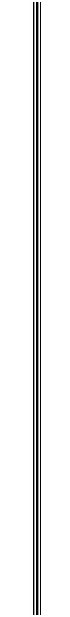
\includegraphics[scale=1.5]{CAPITULOS/PORTADA/barra2} \\[5mm]
    
\includegraphics[scale=0.3]{CAPITULOS/PORTADA/upiita}
\end{flushright}%
\end{minipage}\hfill{}%
\begin{minipage}[t][0.8\paperheight][s]{0.86\columnwidth}%
\begin{center}
    \textbf{\huge Instituto Politécnico Nacional} \\[1cm]
    \textbf{\Large Unidad Profesional Interdisciplinaria en Ingeniería y Tecnologías Avanzadas} \\[1cm]
    \textbf{\large Proyecto Terminal 1} \\[1cm]
    {\large Sistema de reconocimiento de señas de detección de palabras para el lenguaje de señas LSM} \\[1cm]
    \emph{Que para obtener el título de} \\[1cm]
    \textbf{\large ``Ingeniero en Telemática''} \\[1cm]
    \emph{Presenta:} \\[1cm]
    {\large Jose Daniel Alvarez Ramos} \\[1cm]
    \emph{Asesor(es):} \\[1cm]
    {\large Dr. en C. Bella C. Martínez Seis} \\[1cm]
\end{center}
\end{minipage}

% Añadimos el texto alineado a la derecha a la altura de la imagen "upiita"
\vspace{-2cm} % Ajustamos este valor para alinearlo con la imagen
\begin{flushright}
    \textit{México,CDMX, a 10 de octubre de 2024.}
\end{flushright}
\end{table}

\newpage % Nueva página después de la portada
  % Incluye la portada desde el archivo externo

% Índice general
    \tableofcontents
    \newpage

% Índice de figuras
    \addcontentsline{toc}{chapter}{Índice de figuras}
    \listoffigures
    \newpage

% Índice de tablas
    \addcontentsline{toc}{chapter}{Índice de tablas}
    \listoftables
    \newpage

% Índice de ecuaciones
    \listofmyequations  % Llamada a la función que ahora resetea el contador
    \newpage

% Resumen
    \chapter*{Resumen}
    \addcontentsline{toc}{chapter}{Resumen}
    Este proyecto busca desarrollar un sistema que reconozca señas estáticas de la Lengua de Señas Mexicana (LSM) para facilitar la comunicación entre personas con discapacidad auditiva y la comunidad oyente en México. El sistema se basa en la captura de la configuración manual de las señas mediante webcams y utiliza MediaPipe para el seguimiento de las manos. Se enfoca principalmente en el reconocimiento de posturas fijas, con la posibilidad de incluir señas con movimiento si el tiempo lo permite. La traducción precisa de un conjunto predefinido de señas estáticas al español se logrará mediante modelos de aprendizaje profundo, utilizando TensorFlow/Keras. La integración de tecnología en la nube permitirá un procesamiento de datos escalable y una posible traducción en tiempo real. El objetivo final es cerrar la brecha de comunicación entre personas con discapacidad auditiva y oyentes, promoviendo una mayor inclusión y accesibilidad en México.

    \textbf{keywords:}
    Lengua de Señas Mexicana (LSM), Reconocimiento de Señas, Seguimiento de Manos (Hand Tracking), Algoritmos de Aprendizaje Automático, Redes Neuronales Convolucionales (CNN), Redes Neuronales LSTM, Automatización de Procesos, AWS (Amazon Web Services), Sistemas de Mensajería (SQS), Interfaz de Usuario, Análisis de Datos.

% Abstract
    \chapter*{Abstract}
    \addcontentsline{toc}{chapter}{Abstract}
    This project proposes a system for recognizing static signs in Mexican Sign Language (LSM) to facilitate communication between people with hearing disabilities and the hearing community in Mexico. Using webcams for hand tracking and focusing on the manual configuration of signs, the system captures and processes sign language through MediaPipe. The goal is to accurately translate a predefined set of static signs into Spanish, employing deep learning models trained with TensorFlow/Keras. By incorporating cloud technology for scalable data processing and potential real-time translation, this project aims to bridge the communication gap, promoting greater inclusion and accessibility for people with hearing disabilities in Mexico.

    \textbf{Keywords:}
    Accessibility, Computer Vision, Deep Learning, Hand Tracking, Human-Computer Interaction, Mexican Sign Language (LSM), Sign Language Recognition.

% Aquí continúan tus capítulos...
    \chapter{Introducción}

En la actualidad, en México, existen alrededor de 7.1 millones de personas que presentan algún tipo de discapacidad, lo que representa aproximadamente el 6\% de la población total. Estas personas enfrentan desafíos constantes de discriminación en diversas actividades, ya sean laborales, académicas o sociales \cite{ref1}.

Entre este grupo se encuentran personas con hipoacusia, una disminución significativa de la capacidad auditiva, quienes han utilizado históricamente la lengua de señas como su principal medio de comunicación. En México, la Lengua de Señas Mexicana (LSM) y la Lengua de Señas Maya Yucateca (LSMY) son las dos lenguas más reconocidas para este propósito, con la LSM siendo la más utilizada por aproximadamente 87,000 a 100,000 señantes y declarada como lengua nacional desde 2003 \cite{ref2}.

El presente sistema se propone como una herramienta de apoyo a personas con hipoacusia, facilitando la traducción de señas de la LSM a palabras en español mexicano, bajo el código ISO 639-2 sgn-MX. En esta solución se incorporan tecnologías más avanzadas y escalables como MediaPipe para el seguimiento y procesamiento de los movimientos de las manos \cite{ref3}, junto con TensorFlow/Keras para la creación de modelos de aprendizaje profundo que permiten una mayor precisión en la interpretación de las señas \cite{ref4}. La integración de servicios en la nube, como AWS S3 y SQS, también garantiza la escalabilidad y el procesamiento de los datos \cite{ref5}.

Al integrar una API de Text-To-Speech u otras alternativas similares, genera un sistema versátil que convierte las señas en palabras tanto visuales como auditivas, ofreciendo una interacción más inclusiva.
\clearpage
\section{Planteamiento del problema}

Las personas que cuentan con la condición de hipoacusia tienen la perentoriedad de recurrir a herramientas, en su mayoría tecnológicas, que les ayuden o permitan entablar contacto con una inmensa mayoría que desconoce su modo de comunicación \cite{ref6}. Estas personas enfrentan desafíos significativos al comunicarse con quienes no conocen la lengua de señas, lo que limita sus interacciones sociales, laborales y educativas, creando barreras que dificultan su inclusión en la sociedad \cite{ref10}. Aunque existen herramientas que facilitan la traducción de español a Lengua de Señas Mexicana (LSM), la traducción inversa de LSM a español sigue siendo un área poco explorada, con un gran potencial de mejora \cite{ref12}.

Una forma de cerrar esta brecha de comunicación es identificar la palabra que corresponde a la seña interpretada. Para ello, se han creado diversas herramientas lingüísticas, siendo el diccionario una de las principales, donde cada palabra es representada por una o varias imágenes y una descripción escrita que presenta el paso a paso para realizar la seña \cite{ref15}.

En el marco tecnológico, uno de los principales retos es la correcta interpretación de las señas. El uso de sensores presenta oportunidades; sin embargo, herramientas como Kinect no son suficientes debido a sus limitaciones en la detección precisa de las posiciones de las manos \cite{ref14}. Dispositivos como Leap Motion ofrecen una mejor captura de los movimientos, pero aún se necesita desarrollar un sistema que interprete las señas de manera efectiva \cite{ref13}.

Para abordar esta problemática, proponemos un sistema innovador que utiliza tecnologías avanzadas como MediaPipe y TensorFlow/Keras. El objetivo primordial de este sistema es enfocarse en las señas de detención estática. Sin embargo, este es solo el primer paso; se prevé que en caso de contar con tiempo, se podrían incluir otros tipos de señas a través de video (secuencia de fotogramas). Ejemplos de estas otras señas podrían incluir saludos, preguntas básicas o expresiones emocionales. El proceso inicia con el usuario grabando su comunicación en LSM mediante un programa que captura video o imágenes.
Estos archivos de fotogramas son enviados a un almacenamiento en la nube para su procesamiento.

A través de un microservicio, los fotogramas se procesan para extraer puntos clave que representan las señas, utilizando principalmente la captura de las manos mediante MediaPipe. Estos puntos clave se visualizan en la secuencia de fotogramas representativa de la seña o en la imagen, facilitando la identificación de las posiciones y movimientos correspondientes. Estos datos son empleados para entrenar un modelo de aprendizaje profundo que mejora la precisión de la traducción de LSM a español \cite{ref9}. Una vez entrenado, el modelo permite al usuario traducir las señas que se capturan a través de una cámara.

El sistema no solo genera una representación visual de la palabra traducida en pantalla, sino que también utiliza una API (de Text-To-Speech o similar) para reproducir el audio correspondiente, facilitando así una comunicación inclusiva y efectiva \cite{ref11}. Este enfoque integral no solo cierra la brecha comunicativa, sino que también empodera a las personas con hipoacusia, brindándoles herramientas que fomentan su participación en la sociedad.
\clearpage
\section{Propuesta de solución}

\subsection{Descripción del sistema}



En la Figura \ref{fig:diagrama_sistema}, se observa el principio básico del funcionamiento del sistema:

\begin{enumerate}
\item Iniciar Grabación o toma de la muestra: El usuario inicia el programa de grabación o toma de fotos.
\item Captura de Video (secuencia de fotos representativa de la seña) o Fotos: El programa de grabación utiliza la cámara para capturar video o fotos.
\item Dividir en Fotogramas: El video capturado se divide en fotogramas para un análisis más fácil.
\item Almacenamiento Local: Los fotogramas se almacenan temporalmente en el almacenamiento local.
\item Subir Fotogramas a S3: Los fotogramas se suben al servicio de almacenamiento en la nube (AWS S3).
\item Notificación de Nuevo Archivo: EventBridge notifica que se ha subido un nuevo archivo a S3.
\item Invocar Función Lambda: EventBridge invoca una función en AWS Lambda para procesar los fotogramas.
\item Obtener Fotogramas: La función Lambda obtiene los fotogramas desde S3.
\item Enviar Paquete de Fotogramas a SQS: Lambda envía un paquete de 30 fotogramas (URLs de los archivos en S3) a una cola de mensajes (SQS).
\item Recibir Datos en Microservicio: El microservicio recibe los datos desde SQS (Comienza con la descarga de los mismos desde S3).
\item Procesar Frames con MediaPipe: MediaPipe procesa los fotogramas para detectar puntos clave (señas).
\item Enviar DataFrame: El microservicio envía el DataFrame resultante.
\item Entrenar Modelo: Un entrenador recibe el DataFrame y utiliza TensorFlow/Keras para entrenar el modelo de traducción.
\item Guardar Pesos del Modelo: Los pesos entrenados se guardan en el almacenamiento.
\item Iniciar Traducción por el Usuario: El usuario inicia el programa de traducción.
\item Capturar Frames en Tiempo Real o Foto: Se captura frames en foto o tiempo real mediante una cámara local o WebSocket.
\item Predecir Palabra: El modelo predice la palabra correspondiente a las señas capturadas.
\item Mostrar Palabra en Pantalla: La palabra traducida se muestra en la pantalla.
\item Genera Audio con Text-To-Speech: Se envía la palabra a una API de Text-To-Speech para generar audio.
\item Reproducir Audio en Altavoz: El audio generado se reproduce a través de un altavoz.
\end{enumerate}

% ---  Ajusta el caption para que sea vertical ---

\begin{figure}[h]
  \begin{sideways}
   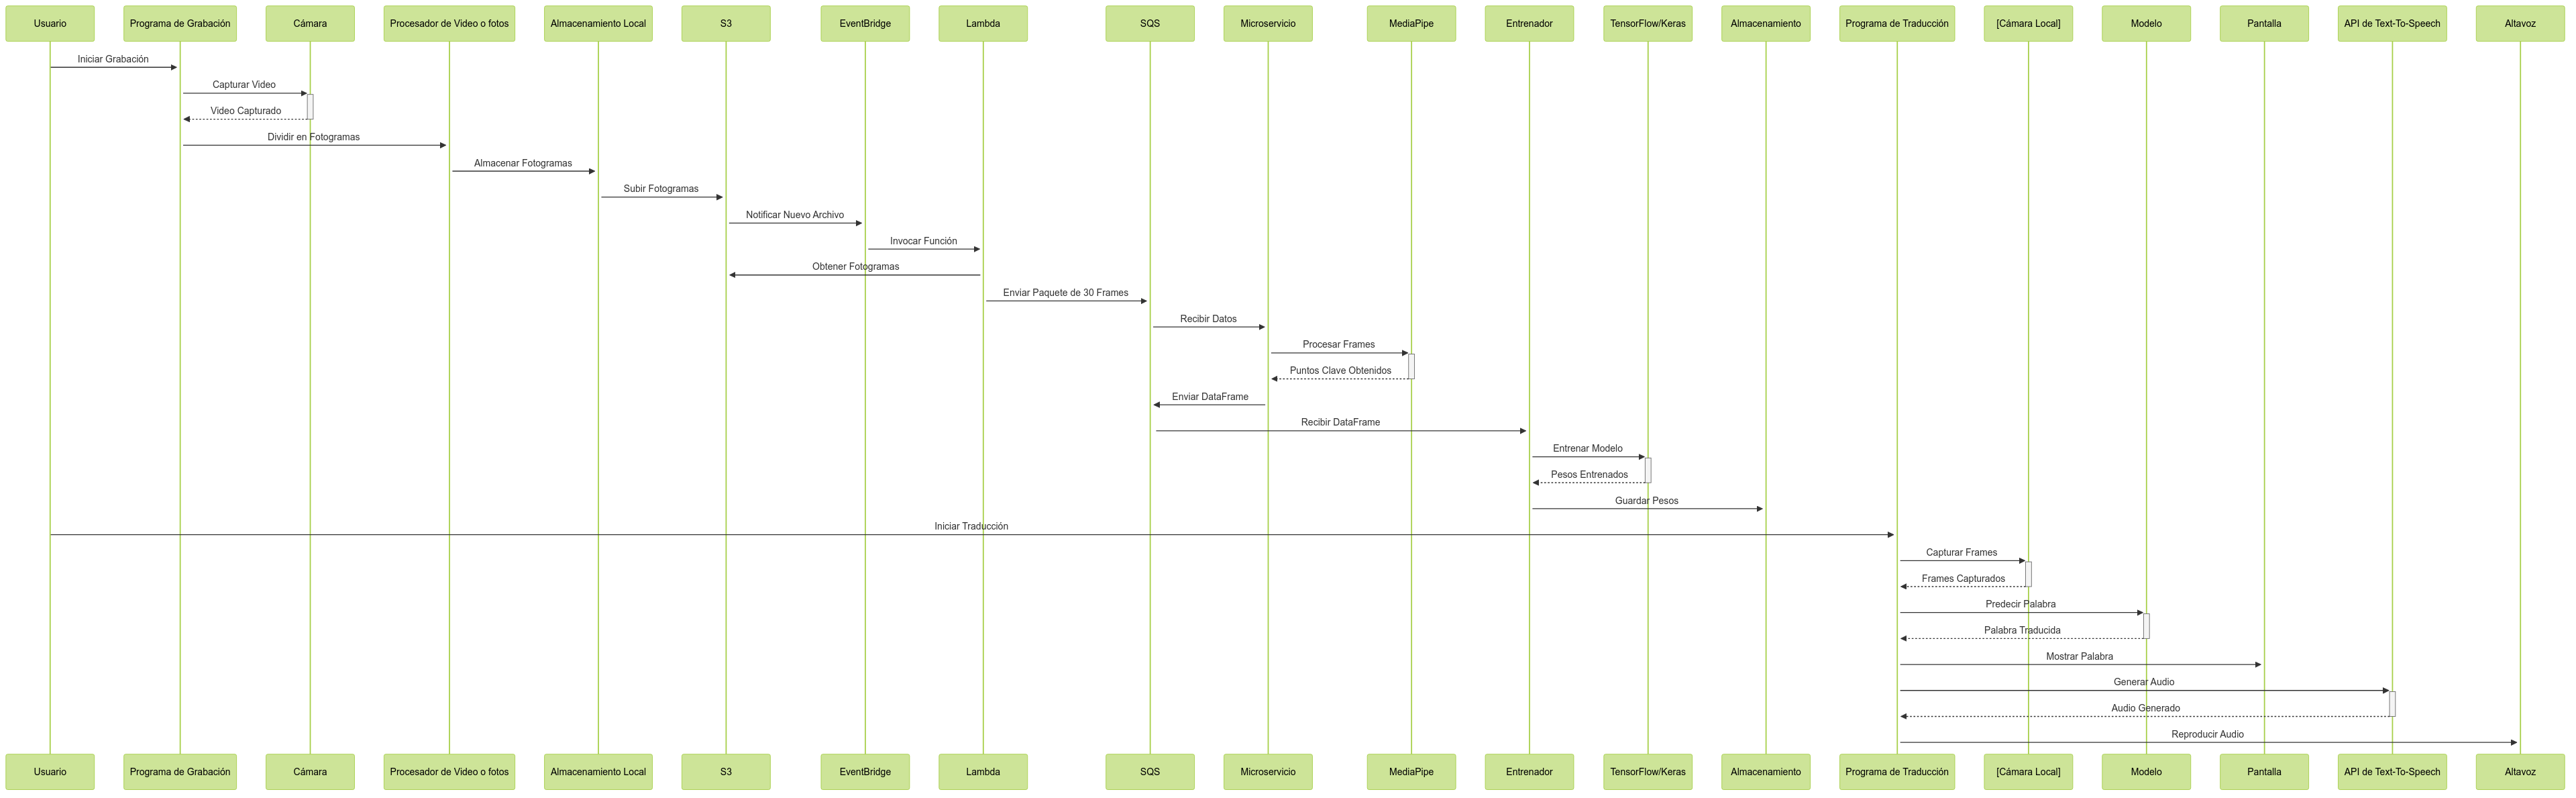
\includegraphics[scale=0.17]{CAPITULOS/capitulo1/digramacap1.png}
  \end{sideways}
  \centering
  \caption[Diagrama del funcionamiento del sistema]{Diagrama del funcionamiento del sistema}
  \label{fig:diagrama_sistema}
\end{figure}



\clearpage


\section{Alcances y limitaciones}


En resumen, los resultados que se esperan ser obtenidos son los siguientes:

\begin{itemize}
    \item \textbf{Reconocimiento de Señas Estáticas:} El sistema se enfocará en el reconocimiento preciso de un conjunto predefinido de señas estáticas de detención dentro de la Lengua de Señas Mexicana (LSM).
    \item \textbf{Ambiente Controlado:} El sistema funcionará de manera óptima en un ambiente interior sin incidencia directa de luz solar, para garantizar la calidad de la captura de imágenes por la cámara y la API de hand tracking.
    \item \textbf{Configuraciones Manuales:} Se deberá contar con configuraciones manuales otorgadas por la API de hand tracking, las cuales constituyen una característica importante, como la posición de manos y los dedos.
    \item \textbf{Señas de Convención:} Existe una similitud léxica alrededor del país de 80\% a 90\%, esto quiere decir que existe una variación dialectal, de acuerdo con la región del país, lo que se buscará es solo utilizar señas como convención por la mayoría de sordos \cite{ref22}.
    \item \textbf{Reconocimiento de Manos y Muñeca:} El sistema se limitará al reconocimiento de manos y muñeca, dentro del espectro permisible para la cámara y la API de hand tracking.
\end{itemize}

\section*{Limitaciones del Sistema}

Por el contrario, es pertinente mencionar lo que no se pretende con este sistema:

\begin{itemize}
    \item \textbf{No Reconocimiento de Frases o Textos:} El sistema no busca hacer reconocimiento de frases, o textos de mayor envergadura únicamente de palabras, dado a que la estructura gramatical de la LSM es muy diferente al español, cabe hacer mención que existe el español signado, pero no este no está dentro del enfoque en la problemática a solucionar \cite{ref21}.
    \item \textbf{No Deletreo:} Tampoco se busca hacer el reconocimiento de palabras por medio de deletreo, dado que ya existen sistemas que realizan esta tarea, de igual manera no representa una manera eficiente de expresarse.
\end{itemize}
\section{Justificación}

En México, el 33.5\% de las personas con discapacidad tiene una discapacidad auditiva y un 18\% presenta dificultades del habla, lo que significa que más del 51\% de este grupo se beneficiaría directamente de herramientas que faciliten la comunicación (Instituto Nacional de Estadística y Geografía \cite{ref1}. 
Para los miles de personas que dominan la Lengua de Señas Mexicana (LSM), este proyecto proporciona una plataforma que les permite transmitir mensajes a quienes no están familiarizados con esta lengua, enfatizando su importancia para la inclusión social \cite{ref16}.
Los estudios muestran que las personas con hipoacusia que tienen un nivel educativo más alto suelen tener un mayor dominio del español, debido a su acceso a recursos como libros e internet. Sin embargo, la falta de señas para ciertos conceptos limita su capacidad comunicativa, lo que a menudo lleva al uso del deletreo de señas en lugar del español signado.
Este trabajo busca desarrollar un sistema de diccionario de palabras en LSM que permita la traducción de señas a palabras en español, apoyado por la tecnología actual \cite{ref17}. Los diccionarios no solo proveen información lingüística, sino que también desempeñan funciones sociales significativas, como fomentar la identidad cultural y cohesionar a la comunidad \cite{ref18}.
La función primordial y más conocida de un diccionario es proveer información sobre una lengua, un diccionario además conlleva otras funciones sociales como dar identidad, función histórica y cohesión de la sociedad \cite{ref19}.
\section{Metodologia}
Para el desarrollo de este sistema de reconocimiento de LSM, se adoptó una metodología ágil inspirada en Scrum, la cual se basa en ciclos iterativos de desarrollo conocidos como sprints. Este enfoque, que prioriza la flexibilidad y la colaboración, se adapta de manera ideal a la naturaleza dinámica del proyecto, permitiendo la incorporación de mejoras y ajustes a lo largo del proceso. La adaptación de Scrum a este proyecto implica un enfoque iterativo en el desarrollo del sistema de reconocimiento de LSM. Se priorizarán las funcionalidades esenciales en los primeros sprints, como la captura y el procesamiento de las señas, y se irán incorporando nuevas funcionalidades, como la integración con la nube y la generación de audio, en sprints posteriores.

Este enfoque se inspira en la práctica descrita por Kniberg (2007), quien destaca varios principios clave de Scrum que aplican directamente a este proyecto\cite{ref39}:

\begin{itemize}
    \item \textbf{Enfoque en la práctica}: Scrum se centra en la aplicación práctica, lo que permite que el equipo se adapte a las necesidades del proyecto de manera eficiente.
    \item \textbf{Adaptabilidad}: La metodología se ajusta al contexto específico del proyecto, permitiendo mayor flexibilidad en lugar de seguir un conjunto rígido de reglas.
    \item \textbf{Colaboración}: La comunicación y colaboración entre el equipo de desarrollo y el Dueño de Producto son esenciales, especialmente durante la planificación de cada sprint.
    \item \textbf{Entrega continua}: Al final de cada sprint, se promueve la entrega de software funcional, asegurando que el producto esté en constante evolución y mejora.
    \item \textbf{Mejora continua}: A través de retrospectivas, el equipo analiza y mejora su proceso en cada sprint.
    \item \textbf{Simplicidad}: El proyecto se gestiona de manera simple, utilizando herramientas como tarjetas físicas para la organización del backlog del producto y del sprint.
    \item \textbf{Transparencia}: La transparencia en el progreso es fundamental, y se asegura mediante un tablón de tareas visible para todo el equipo y una página de información del sprint para mantener informada a toda la organización.
\end{itemize}
En la \ref{fig:imagen_scrum} se presenta un esquema de las etapas que conforman la metodología SCRUM:

\begin{figure}[h]
  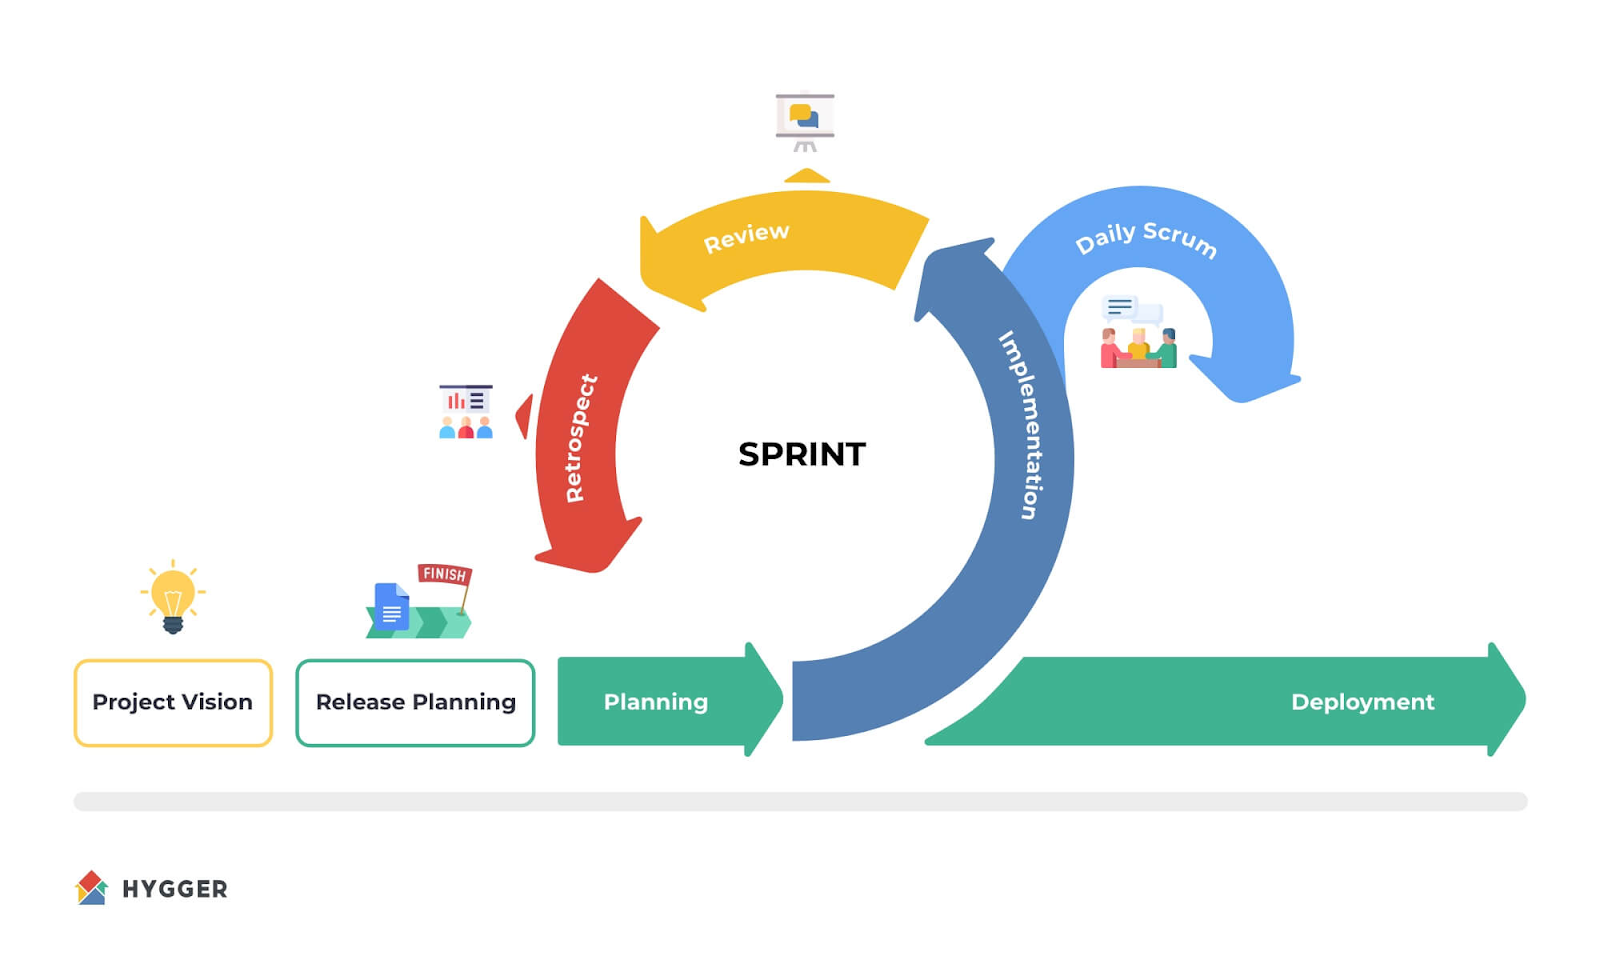
\includegraphics[scale=0.17]{CAPITULOS/capitulo1/scrum.png}
  \centering
  \caption[Metodología Scrum ]{Metodología Scrum \cite{ref40}}
  \label{fig:imagen_scrum}
\end{figure}

\clearpage

\section{Objetivos}

\subsection{Objetivo general}

Desarrollar un sistema de reconocimiento de señas estáticas de la LSM, con una arquitectura híbrida que combine componentes \textit{on-premise} y en la nube. Se utilizará MediaPipe u otra API de \textit{hand tracking} para la captura y procesamiento de datos, enfocándose en señas de configuración manual o de reposo y parametrizando las principales articulaciones manuales en un sistema de coordenadas rectangulares. A partir de estos datos, se entrenará un modelo de clasificación utilizando TensorFlow para reconocer y asociar las señas a su equivalente en español. La palabra reconocida será reproducida utilizando una API de voz (\textit{speech-to-text}).

\subsection{Objetivos específicos}

\begin{enumerate}
    \item \textbf{Recopilación de Datos:}
        \begin{itemize}
            \item Recopilar un conjunto de datos representativo de señas estáticas de detención en LSM, incluyendo variaciones dialectales comunes, y etiquetarlas con su significado en español.
            \item Utilizar una cámara web para capturar de las señas, asegurando una calidad adecuada en un ambiente controlado. Extraer una secuencia de fotogramas representativa de cada seña para su posterior procesamiento.
            \item Utilizar MediaPipe para extraer los puntos clave de las articulaciones de las manos en un sistema de coordenadas rectangulares.
        \end{itemize}

    \item \textbf{Modelado y Entrenamiento:}
        \begin{itemize}
            \item Seleccionar y adaptar un modelo de reconocimiento existente, como una red neuronal convolucional (CNN), para el reconocimiento de señas estáticas \cite{ref7}.
            \item Entrenar un modelo de reconocimiento de señas utilizando técnicas de aprendizaje automático (TensorFlow/Keras) con los datos recopilados y etiquetados.
        \end{itemize}

    \item \textbf{Diseño del Almacenamiento de Datos:}
        \begin{itemize}
            \item Diseñar e implementar una estructura de almacenamiento eficiente que combine una base de datos y un \textit{bucket} (como S3) para gestionar la información recopilada. La base de datos almacenará metadatos de las señas (traducciones, parámetros de articulaciones, configuraciones manuales), mientras que el \textit{bucket} almacenará las imágenes de las señas. Se asegurará la integridad de los datos y se facilitará el acceso a ambos tipos de información para el entrenamiento, la ejecución y el mantenimiento del sistema.
        \end{itemize}

    \item \textbf{Desarrollo de la Salida y Configuración:}
        \begin{itemize}
            \item Implementar un mecanismo de salida claro y accesible para presentar la traducción de la seña reconocida, ya sea en texto, audio (utilizando una API de \textit{Text-To-Speech}) o ambos, según los requisitos del usuario final.
            \item Considerar la posibilidad de desarrollar una interfaz web intuitiva para interactuar con el sistema, si los recursos y el alcance del proyecto lo permiten.
        \end{itemize}
\end{enumerate}
    \chapter{Marco Teórico}

\section{Medidas de tendencia central}

Las medidas de tendencia central son herramientas estadísticas que nos permiten resumir la localización de los datos, es decir, nos ayudan a identificar el valor alrededor del cual se centran los datos. Estas medidas son esenciales para el análisis de datos en cualquier investigación, incluyendo el análisis de las muestras de Lengua de Señas Mexicana (LSM).

\textbf{Medidas de tendencia central:}

\textbf{Media:}

La media aritmética es el valor obtenido al sumar todos los valores de un conjunto de datos y dividir entre el número de datos. En el análisis de LSM, la media puede utilizarse para calcular la posición promedio de las manos en una seña.

\indexedequation{Media aritmética}{
\begin{equation}
    \bar{x} = \frac{\sum_{i=1}^{n} x_i}{n}
    \label{eq:media}
\end{equation}
}


\textbf{Varianza:}

La varianza es una medida de dispersión que indica cuánto varían los datos alrededor de la media. Una varianza alta indica que los datos están más dispersos, mientras que una varianza baja indica que los datos están más agrupados alrededor de la media.

La fórmula para calcular la varianza es:
\indexedequation{Varianza}{
    \begin{equation}
        \sigma^2 = \frac{\sum_{i=1}^{n} (x_i - \bar{x})^2}{n-1}
        \label{eq:varianza}
    \end{equation}
}


\textbf{Desviación Estándar:}

La desviación estándar es una medida de dispersión que indica cuánto varían los datos alrededor de la media. Una desviación estándar alta indica que los datos están más dispersos, mientras que una desviación estándar baja indica que los datos están más agrupados alrededor de la media.

La fórmula para calcular la desviación estándar es:
\indexedequation{Desviación estándar}{
\begin{equation}
    \sigma = \sqrt{\frac{\sum_{i=1}^{n} (x_i - \bar{x})^2}{n-1}}
    \label{eq:desviacion_estandar}
\end{equation}
}

\section{MediaPipe Holistic}

MediaPipe Holistic es una solución integral de Google para el seguimiento del cuerpo humano en tiempo real. El modelo de Holistic combina  modelos de aprendizaje profundo para detectar y rastrear puntos (posiciones flotantes en un  plano x, y) clave en el rostro, las manos y el cuerpo completo. Esta capacidad de análisis detallado de los movimientos corporales es esencial para la captura expresiva de la Lengua de Señas Mexicana (LSM), donde la posición del cuerpo y los movimientos de las manos son fundamentales para recibir y generar la comunicación.

\subsection{Componentes del Modelo Holistic}

MediaPipe Holistic se compone de tres modelos principales:

\begin{enumerate}
    \item \textbf{Pose Landmarker:}
    \begin{itemize}
        \item \textbf{Descripción:}  Este modelo detecta 33 puntos de referencia del cuerpo humano en una imagen o video, incluyendo la nariz, los ojos, las orejas, los hombros, los codos, las muñecas, las caderas, las rodillas y los tobillos. 
        \item \textbf{Aplicaciones en lengua de señas mexicana:}  Estos puntos son cruciales para interpretar las señas, ya que permiten analizar la postura general del cuerpo y la posición de los brazos y las manos en relación al torso. Por ejemplo, la posición de los codos y las muñecas es fundamental para distinguir señas como \textquotedblleft CASA\textquotedblright  u  \textquotedblleft HOLA\textquotedblright.
        \item \textbf{Funcionamiento:} El modelo utiliza una red neuronal convolucional similar a MobileNetV2 y está optimizado para aplicaciones de entrenamiento en tiempo real y en el dispositivo.  Primero, detecta la presencia de cuerpos humanos en la imagen, y luego localiza los 33 puntos de referencia en el cuerpo detectado.
        \item \textbf{Opciones de configuración:}  
            \begin{itemize}
                \item \textbf{running\_mode:} Establece el modo de ejecución (IMAGE, VIDEO, LIVE\_STREAM).
                \item \textbf{num\_poses:} La cantidad máxima de poses a detectar.
                \item \textbf{min\_pose\_detection\_confidence:} Puntuación mínima para la detección de poses.
                \item \textbf{min\_pose\_presence\_confidence:} Puntuación mínima de presencia de poses.
                \item \textbf{min\_tracking\_confidence:} Puntuación mínima para el seguimiento de poses.
                \item \textbf{output\_segmentation\_masks:}  Si se generan máscaras de segmentación.
            \end{itemize}
    \end{itemize}
    \begin{figure}[h]
        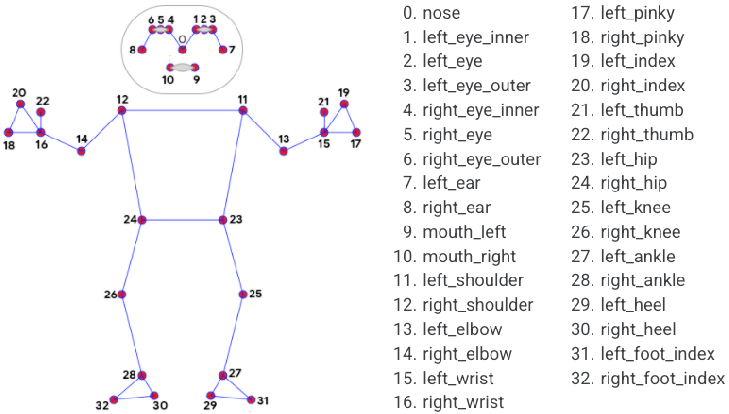
\includegraphics[scale=0.4]{CAPITULOS/capitulo2/img.png}
        \centering
        \caption[Puntos de medipipe]{Puntos de medipipe Pose Landmarker \cite{ref20}}
        \label{fig:imagen_medipipe_pose}
    \end{figure}
    \item \textbf{Face Landmarks:}
    \begin{itemize}
        \item \textbf{Cantidad:} 468 puntos.
        \item \textbf{Descripción:}  Detecta puntos clave en el rostro, como los ojos, las cejas, la nariz, la boca y el contorno de la cara.
        \item \textbf{Aplicaciones de MediaPipe Holistic en el sistema:} Se utilizan para analizar las expresiones faciales, que son un componente gramatical crucial en la LSM. Por ejemplo, las expresiones faciales pueden indicar preguntas, negación, o emociones.
    \end{itemize}

    \item \textbf{Hand Landmarks:}
    \begin{itemize}
        \item \textbf{Cantidad:} 21 puntos por cada mano \cite{ref20}.
        \item \textbf{Descripción:} Detecta  puntos clave en las manos, como las puntas de los dedos, los nudillos y la palma.
        \item \textbf{Aplicaciones de MediaPipe Holistic en el sistema:} Permite analizar la forma, orientación y movimiento de las manos, lo cual es fundamental para identificar los diferentes queremas (formas de la mano) en la LSM.
    \end{itemize}
    \begin{figure}[h]
              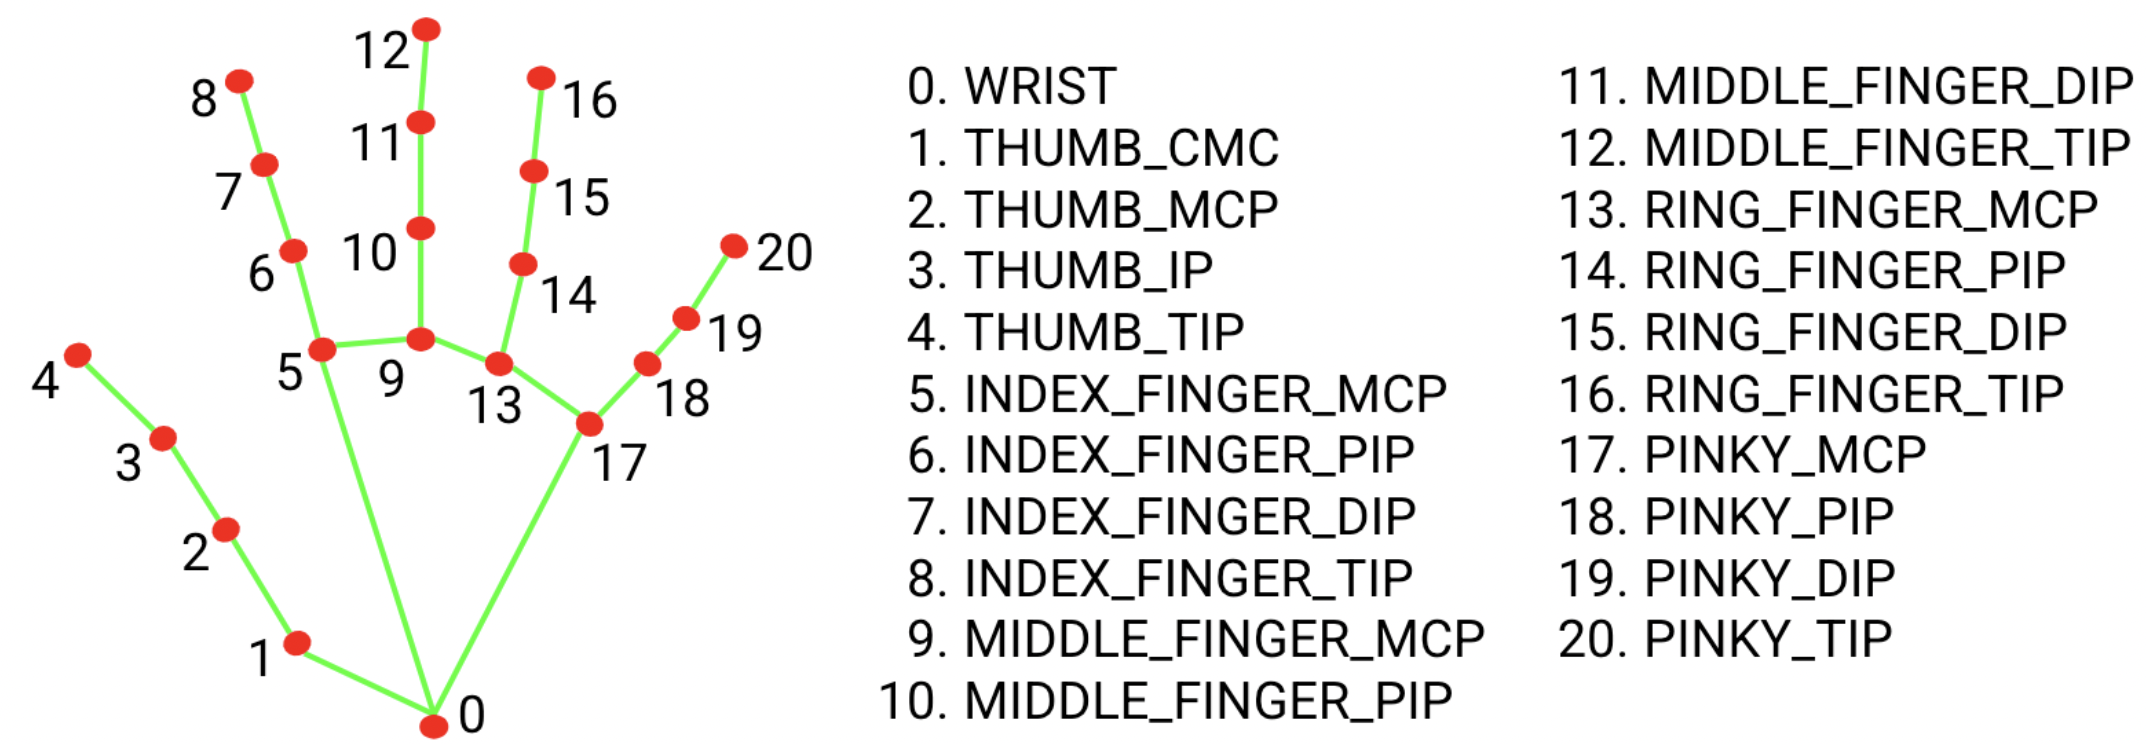
\includegraphics[scale=0.4]{CAPITULOS/capitulo2/hand-landmarks.png}
              \centering
              \caption[Puntos de medipipe ]{Puntos de medipipe Hand Landmarks\cite{ref20}}
              \label{fig:imagen_medipipe_hand}
    \end{figure}

\end{enumerate}




\subsection{Ventajas de MediaPipe Holistic}

\begin{itemize}
\item \textbf{Integración completa:} Combina el seguimiento de rostro, manos y cuerpo en un solo framework, lo que facilita el desarrollo de aplicaciones de LSM.
\item \textbf{Rendimiento en tiempo real:} Permite procesar imágenes en tiempo real, lo que es crucial para la fluidez en la traducción de LSM.
\item \textbf{Eficiencia computacional:} Está optimizado para ejecutarse en dispositivos móviles y de escritorio, con bajo consumo de recursos.
\item \textbf{Robustez:} Funciona en diferentes condiciones de iluminación y con diferentes tipos de cámaras.
\item \textbf{Facilidad de uso:} MediaPipe ofrece APIs fáciles de usar para integrar Holistic en aplicaciones de Python, Android y web.
\end{itemize}

\section{TensorFlow/Keras}
TensorFlow, una plataforma de aprendizaje automático de código abierto, y Keras, una interfaz de alto nivel para construir y entrenar modelos de redes neuronales, son herramientas esenciales en el desarrollo de modelos de aprendizaje profundo. Estos modelos, entrenados con datos de LSM, son capaces de reconocer y clasificar señas, formando la base del sistema de traducción \cite{ref34}.

\section{Procesamiento Híbrido (Local y en la Nube)}
El enfoque híbrido combina el procesamiento local en el dispositivo del usuario con el procesamiento en la nube a través de Amazon Web Services (AWS). Esta estrategia aprovecha las ventajas de ambos entornos: el procesamiento local reduce la latencia y protege la privacidad, aspectos cruciales al tratar con datos sensibles como la comunicación en LSM, mientras que la nube ofrece potencia de cómputo escalable para tareas intensivas, como el entrenamiento de modelos y el almacenamiento de datos \cite{ref35}.

\section{Amazon Web Services (AWS)}
AWS proporciona una amplia gama de servicios en la nube que son fundamentales para el proyecto:
\begin{itemize}
    \item \textbf{Buckets S3:} Almacenamiento escalable y seguro para grandes volúmenes de datos de LSM, como videos y modelos de aprendizaje profundo.
    \item \textbf{Colas SQS:} Facilitan la comunicación asincrónica entre los diferentes microservicios del sistema, permitiendo el procesamiento eficiente y desacoplado de solicitudes de traducción.
    \item \textbf{Funciones Lambda:} Ejecutan código sin necesidad de aprovisionar o administrar servidores, lo que permite escalar automáticamente el procesamiento de solicitudes de traducción según la demanda \cite{ref5}.
\end{itemize}

\section{Lingüística de la Lengua de Señas Mexicana (LSM)}
La LSM, como cualquier lengua natural, posee una gramática compleja que incluye aspectos como la configuración manual, la ubicación, la orientación y el movimiento de las manos, así como las expresiones faciales. El proyecto incorpora conocimientos lingüísticos de la LSM para asegurar una traducción precisa y culturalmente apropiada. La Matriz Segmental, que describe la estructura de las señas en términos de segmentos secuenciales, es una herramienta clave para el análisis y la representación de las señas en el sistema \cite{ref36}.

\subsection{Composición de una seña en la Lengua de Señas Mexicana (LSM)}

La Lengua de Señas Mexicana (LSM), al igual que otras lenguas de señas, se caracteriza por ser una lengua visual-gestual donde la información se transmite a través de la combinación de movimientos y configuraciones de las manos, expresiones faciales y movimientos del cuerpo. Para comprender la estructura de la LSM, es fundamental analizar los elementos que componen una seña.  \cite{ref42}

Una seña en LSM se compone de la articulación simultánea de tres matrices principales:

\subsection{Matriz Segmental:}

Esta matriz se centra en la descripción de la actividad manual,  analizando el movimiento y la detención de la mano.

\begin{itemize}
    \item \textbf{Segmentos:} Se distinguen dos tipos de segmentos:
    \begin{itemize}
        \item \textbf{Movimiento (M):}  Existe un cambio en la configuración o ubicación de la mano en el espacio.
        \item \textbf{Detención (D):} La mano mantiene su posición sin cambios.
    \end{itemize}

    \item \textbf{Tipos de movimiento:}
    \begin{itemize}
        \item \textbf{Movimientos de contorno:}  Describen una trayectoria en el espacio, como lineal, arco, círculo, zigzag, etc.
        \item \textbf{Movimientos locales:} No describen una trayectoria espacial, como movimientos ondulatorios, circulares o de cabeceo.
    \end{itemize}

    \item \textbf{Cualidades de los rasgos:}
    \begin{itemize}
        \item \textbf{Temporal:} Describe la duración del movimiento (sostenido, abreviado, lento, etc.).
        \item \textbf{No temporal:} Describe alteraciones físicas en la ejecución del movimiento (tenso, menguado, ampliado).
        \item \textbf{Contacto:} Describe la relación de proximidad entre la mano y otra parte del cuerpo o el espacio (rozando, rebote).
    \end{itemize}

    \item \textbf{Cualidad espacial:} Describe la orientación de la trayectoria del movimiento en el espacio (plano horizontal, vertical, etc.).
\end{itemize}


\subsection{Matriz Articulatoria:}

Esta matriz describe la postura de la mano en la producción de la seña, considerando diferentes parámetros:

\begin{itemize}
    \item \textbf{Configuración de la mano (CM):} Especifica la forma que adopta la mano, incluyendo la posición de los dedos y el pulgar.  Por ejemplo, mano extendida, mano en puño, dedos flexionados, etc.

    \item \textbf{Ubicación (UB):} Indica el lugar donde se realiza la seña con respecto al cuerpo o el espacio de señalización. Puede ser en la frente, la cabeza, el pecho, el espacio neutro frente al cuerpo, etc.

    \item \textbf{Dirección (DI):} Indica hacia dónde se dirige la palma de la mano durante la ejecución de la seña.  Las opciones incluyen palma arriba, palma abajo, palma hacia el cuerpo, palma hacia afuera, etc.

    \item \textbf{Orientación (OR):} Describe la orientación de la mano con respecto al plano horizontal.  Puede ser con la palma hacia arriba (base), la palma hacia abajo (dorso), o con la palma lateral.
\end{itemize}

\subsection{Matriz de Rasgos No Manuales (RNM):}

Esta matriz se refiere a los elementos no manuales que acompañan la producción de la seña y que contribuyen a su significado.

\begin{itemize}
    \item \textbf{Expresiones faciales:} Incluyen movimientos de las cejas (levantadas, fruncidas), ojos (abiertos, cerrados), nariz (arrugada), boca (sonrisa, labios fruncidos) que modifican la interpretación de la seña.

    \item \textbf{Movimientos de la cabeza:}  Involucran movimientos como el cabeceo (afirmación, negación), la inclinación lateral, o la rotación de la cabeza, que complementan el significado de la seña.

    \item \textbf{Posturas del cuerpo:} Se refiere a la posición general del cuerpo durante la señalización, como la inclinación del torso, los hombros encogidos, etc.
\end{itemize}



\section{ Arquitectura de Microservicios}
El proyecto adopta una arquitectura de microservicios en la parte del entrenamiento del modelo, donde cada componente del sistema se implementa como un servicio independiente y autónomo. Esta modularidad facilita el desarrollo, la implementación y el mantenimiento del sistema, permitiendo escalar y actualizar componentes individuales sin afectar el funcionamiento global \cite{ref37}.

\section{Redes Neuronales}
Las redes neuronales son un conjunto de algoritmos inspirados en la estructura del cerebro humano, diseñados para reconocer patrones. Se componen de nodos interconectados, organizados en capas, que procesan y transmiten información.
\subsection{Redes Neuronales Convolucionales (CNN)}

Las Redes Neuronales Convolucionales (CNN) son una red neuronal profunda con gran eficacia en el procesamiento de imágenes y videos. Esta capacidad se debe a su estructura, enfoca analizar datos organizados en forma de grilla, como es el caso de las imágenes. En el contexto de la traducción de la Lengua de Señas Mexicana (LSM), las CNN tienen un rol fundamental, ya que facilitan el análisis de las imágenes que capturan las señas realizadas por el usuario.

Las CNN se caracterizan por la inclusión de capas convolucionales. Estas capas emplean filtros (kernels), que se deslizan sobre la imagen de entrada para identificar y extraer características relevantes.


\section{Convolución: Definición General}

La convolución  se puede definir como la integral del producto de dos funciones después de desplazar una de ellas una distancia $t$, como se observa en la ecuación \ref{eq:convolucion_continua}:


\indexedequation{Convolucion Definición general}{
    f(x) = \begin{equation}
               S(t) = \int_{-\infty}^{\infty} x(a)w(t-a) da
               \label{eq:convolucion_continua}
    \end{equation}
}



donde:

\begin{itemize}
    \item  $x(a)$ Es la señal de entrada (entrada de la red).
    \item  $w(t-a)$ Es la segunda función (kernel) desplazada una distancia $t$.
    \item  $S(t)$ Es la función resultante de operar la convolución.
\end{itemize}

La salida ($S$) se conoce como mapa de características.


\subsection{Convolución Discreta}

Al tener que procesar datos en una computadora, el tiempo y la señal de entrada se discretizan.  En consecuencia, la operación de convolución se adapta al dominio discreto, como se expresa en la ecuación \ref{eq:convolucion_discreta}:

\indexedequation{Convolucion Discreta}{
    \begin{equation}
        S(t) = (x * w)(t) = \sum_{a = -\infty}^{\infty} x(a)w(t-a)
        \label{eq:convolucion_discreta}
    \end{equation}
}





\subsection{Convolución en 2 Dimensiones}

Las imágenes son datos bidimensionales, por lo que la convolución se extiende a dos dimensiones. Si $I$ representa la imagen de entrada y $K$ representa el kernel, la convolución 2D se define como:

\indexedequation{Convolución en 2 Dimensiones}{
    \begin{equation}
        S(i,j) = (I * K)(i,j) =  \sum_{m} \sum_{n} I(m,n) K(i-m, j-n)
        \label{eq:convolucion_2d}
    \end{equation}
}



donde:

\begin{itemize}
    \item $S(i,j)$ representa el valor del píxel en la posición $(i,j)$ del mapa de características de salida.
    \item $I(m,n)$ representa el valor del píxel en la posición $(m,n)$ de la imagen de entrada.
    \item $K(i-m,j-n)$ representa el valor del elemento en la posición $(i-m,j-n)$ del kernel.
\end{itemize}

\begin{figure}[h]
    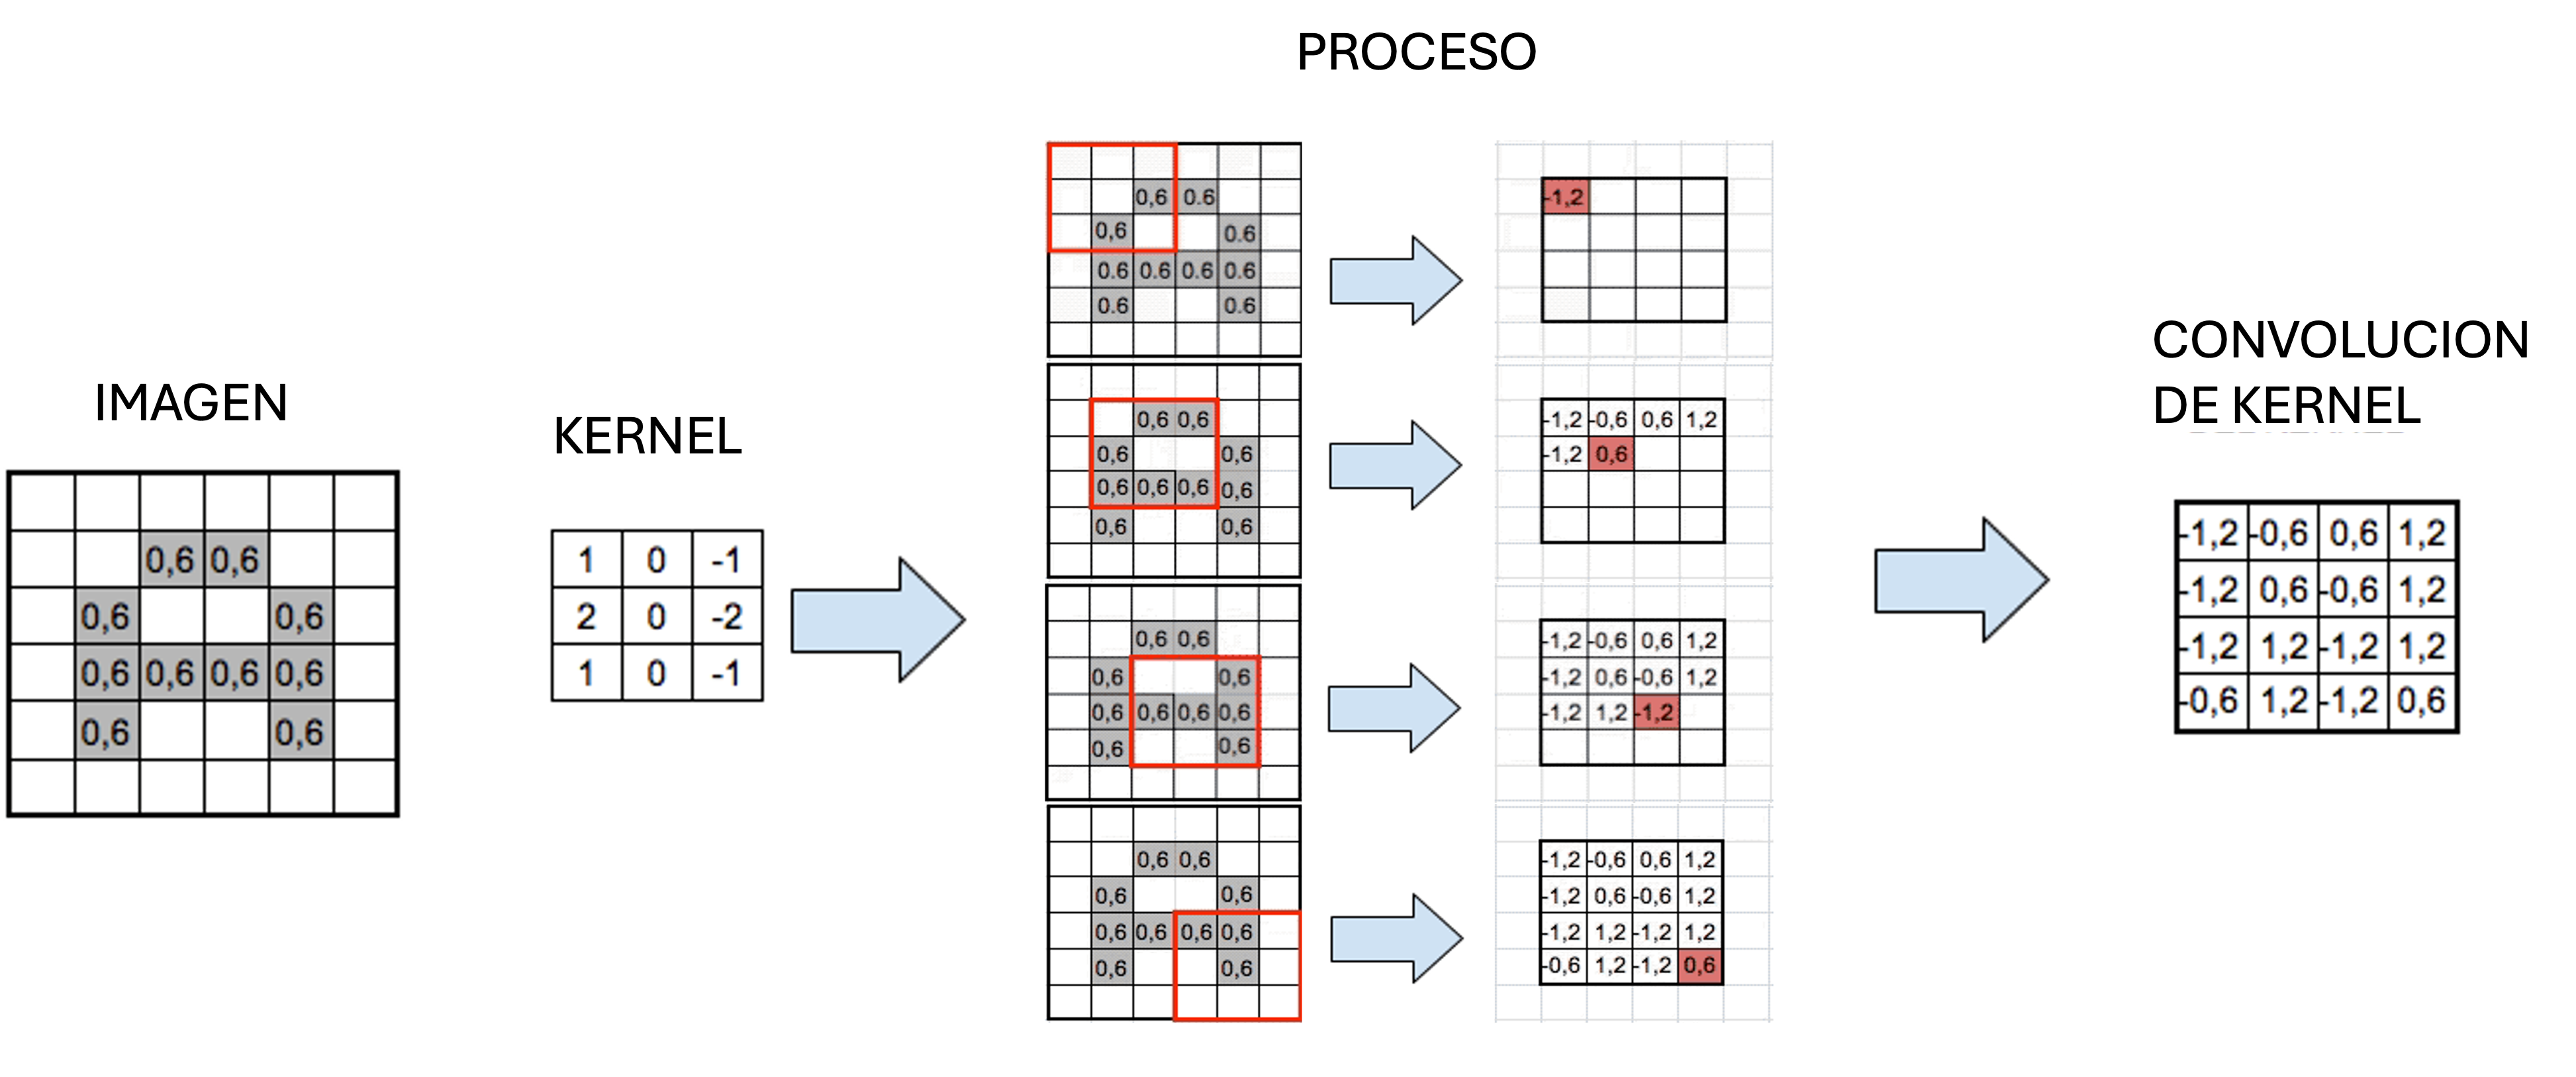
\includegraphics[width=0.9\textwidth]{CAPITULOS/capitulo2/imagenpresentacion}
    \centering
    \caption{Acción de Convolución}
    \label{fig:accion_convolucion}
\end{figure}



De esta manera, se ilustra la transición de la convolución en su forma general a la convolución discreta y, finalmente, a la convolución 2D empleada en las CNN para el procesamiento de imágenes.
\subsection{Redes Neuronales Recurrentes (RNN) para el Análisis de Señas Dinámicas}

Las Redes Neuronales Recurrentes (RNN) constituyen una clase de red neuronal artificial que se caracteriza por sus conexiones recurrentes, lo que les confiere la habilidad de procesar secuencias de datos. Esta propiedad las vuelve especialmente idóneas para el reconocimiento de señas dinámicas en la Lengua de Señas Mexicana (LSM), donde la información temporal es fundamental para la adecuada interpretación del significado. A diferencia de las CNN, que se centran principalmente en el análisis de las características espaciales de las imágenes, las RNN se enfocan en la evolución temporal de las señas, considerando cómo la posición y el movimiento de las manos se modifican a lo largo del tiempo.

\subsubsection{LSTM (Long Short-Term Memory)}

Las LSTM (Long Short-Term Memory) son una variante de las RNN que aborda el problema del desvanecimiento del gradiente, un obstáculo frecuente en el entrenamiento de RNN tradicionales. Este problema dificulta la captura de dependencias a largo plazo en las secuencias de datos. Las LSTM, con su arquitectura de memoria a corto y largo plazo, superan esta limitación y permiten modelar secuencias más extensas y complejas.

\paragraph{Arquitectura de una celda LSTM}

Una celda LSTM está compuesta por tres puertas principales:

\begin{itemize}
    \item \textbf{Puerta de entrada:} Regula la entrada de nueva información a la memoria de la celda.
    \item \textbf{Puerta de olvido:} Determina qué información se descarta de la memoria de la celda.
    \item \textbf{Puerta de salida:}  Controla qué información se utiliza para actualizar el estado oculto de la celda.
\end{itemize}

\paragraph{Ecuaciones de una celda LSTM}

Las siguientes ecuaciones describen el funcionamiento de una celda LSTM:

\begin{align*}
    i_t &= \sigma(W_{xi} x_t + W_{hi} h_{t-1} + b_i) \\
    f_t &= \sigma(W_{xf} x_t + W_{hf} h_{t-1} + b_f) \\
    o_t &= \sigma(W_{xo} x_t + W_{ho} h_{t-1} + b_o) \\
    \tilde{c}_t &= tanh(W_{xc} x_t + W_{hc} h_{t-1} + b_c) \\
    c_t &= f_t * c_{t-1} + i_t * \tilde{c}_t \\
    h_t &= o_t * tanh(c_t)
\end{align*}

donde:

\begin{itemize}
    \item $x_t$: Vector de entrada en el instante $t$.
    \item $h_t$: Estado oculto en el instante $t$.
    \item $c_t$: Estado de la celda en el instante $t$.
    \item $i_t$, $f_t$, $o_t$:  Valores de las puertas de entrada, olvido y salida, respectivamente.
    \item $\tilde{c}_t$:  Candidato al nuevo estado de la celda.
    \item $W_{xi}$, $W_{hi}$, etc.: Matrices de pesos.
    \item $b_i$, $b_f$, etc.: Vectores de sesgo.
    \item $\sigma$: Función sigmoide.
    \item $tanh$: Función tangente hiperbólica.
\end{itemize}

\paragraph{Complemento a la red neuronal convolucional}

En el proyecto de identificación de señas LSM, las LSTM complementan a las CNN al procesar la información temporal de las secuencias de imágenes. Mientras que las CNN extraen características espaciales de cada imagen, las LSTM modelan la evolución de estas características a lo largo del tiempo, capturando la dinámica de las señas. Esta combinación de CNN y LSTM permite un análisis más completo de las señas, mejorando la precisión del sistema de reconocimiento.

En resumen, la incorporación de LSTM en el proyecto de identificación de señas LSM permite un análisis más preciso y robusto de las señas dinámicas, al considerar la información temporal en conjunto con las características espaciales extraídas por las CNN.
\section{Funciones de Activación}
Las funciones de activación introducen no linealidad en las redes neuronales, permitiendo que estas aprendan patrones complejos en los datos. Imaginemos que nuestra red se encuentra ante una bifurcación en el camino; las funciones de activación son responsables de decidir hacia dónde dirigirse.

\subsection{Función Sigmoide}
La función sigmoide transforma cualquier valor de entrada a un rango entre 0 y 1. Esta función es especialmente útil en la capa de salida para problemas de clasificación binaria, como determinar si una seña corresponde a una palabra específica.

\begin{figure}[H]
    \centering
    \begin{tikzpicture}
        \begin{axis}[
            xlabel={$x$},
            ylabel={$\sigma(x)$},
            xmin=-5, xmax=5,
            ymin=-0.2, ymax=1.2,
            legend pos=north west,
            axis lines=middle,
            grid=both,
            minor tick num=4,
        ]
        \addplot[domain=-5:5, samples=100, blue, thick] {1/(1+exp(-x))};
        \legend{Sigmoide}
        \end{axis}
    \end{tikzpicture}
    \caption{Gráfica de la función sigmoide.}
\end{figure}

% Función por partes
\indexedequation{Función de activacion Sigmoide}{
f(x) = \begin{cases}
      \frac{1}{1 + e^{-x}}
   \end{cases} \label{eq:funcion_por_partes_sigmoide}
}


\subsection{Función Tangencial Hiperbólica (tanh)}

La función tangencial hiperbólica, conocida como tanh, es otra función de activación que produce valores en el rango de (-1, 1). A diferencia de la sigmoide, que se limita a valores positivos, tanh puede asignar salidas tanto negativas como positivas. Esto la hace especialmente adecuada para problemas donde es necesario identificar tanto clases positivas como negativas, o en situaciones donde se requiere una salida centrada en cero.

\begin{figure}[H]
    \centering
    \begin{tikzpicture}
        \begin{axis}[
            xlabel={$x$},
            ylabel={$\tanh(x)$},
            xmin=-5, xmax=5,
            ymin=-1.2, ymax=1.2,
            legend pos=north west,
            axis lines=middle,
            grid=both,
            minor tick num=4,
        ]
        \addplot[domain=-5:5, samples=100, blue, thick] {tanh(x)};
        \legend{$\tanh(x)$}
        \end{axis}
    \end{tikzpicture}
    \caption{Gráfica de la función tangencial hiperbólica ($\tanh$).}
\end{figure}

% Función por partes de tanh
\indexedequation{Función de activacion (tanh)}{
f(x) = \begin{cases}
      -1, & \text{si } x \to -\infty \\
      1, & \text{si } x \to +\infty \\
      \tanh(x), & \text{de otra manera}
   \end{cases} \label{eq:tanh}
}

La función tangencial hiperbólica (tanh), se define mediante la siguiente fórmula:

\indexedequation{Definición tanh}{
\tanh(x) = \frac{e^x - e^{-x}}{e^x + e^{-x}} \label{eq:tanh_formula}
}



\subsection{Función ReLU (Rectified Linear Unit)}
La función ReLU es una función lineal que retorna 0 para entradas negativas y el valor de entrada para entradas positivas. Esta función ha ganado popularidad debido a su simplicidad y eficiencia computacional. En el contexto del reconocimiento de señas, ReLU puede ser utilizada en las capas ocultas de la red neuronal para mejorar la capacidad de aprendizaje del modelo.

\begin{figure}[H]
    \centering
    \begin{tikzpicture}
        \begin{axis}[
            xlabel={$x$},
            ylabel={$ReLU(x)$},
            xmin=-5, xmax=5,
            ymin=-0.2, ymax=5,
            legend pos=north west,
            axis lines=middle,
            grid=both,
            minor tick num=4,
        ]
        \addplot[domain=-5:0, samples=100, blue, thick] {0};
        \addplot[domain=0:5, samples=100, blue, thick] {x};
        \legend{ReLU}
        \end{axis}
    \end{tikzpicture}
    \caption{Gráfica de la función ReLU.}
\end{figure}

% Función por partes
\indexedequation{Función de activacion Relu}{
f(x) = \begin{cases}
      0, & \text{si } x < 0 \\
      x, & \text{si } x \geq 0 
   \end{cases} \label{eq:funcion_por_partes_relu}
}

\subsection{Función Softmax}
La función Softmax es frecuentemente utilizada en modelos de clasificación multiclase, ya que convierte las salidas de la red neuronal en probabilidades. Asigna a cada clase una probabilidad que refleja la certeza del modelo sobre su pertenencia, y la clase con la probabilidad más alta se selecciona como la predicción final. Esta función es esencial en muchas redes neuronales profundas, particularmente en la capa de salida de modelos que manejan múltiples categorías.



% Figura para la función Softmax
\begin{figure}[H]
    \centering
    \begin{tikzpicture}
        \begin{axis}[
            xlabel={$z$},
            ylabel={$\sigma(z)_j$},
            xmin=-5, xmax=5,
            ymin=0, ymax=1,
            legend pos=north west,
            axis lines=middle,
            grid=both,
            minor tick num=4
        ]
            % Softmax example with three fixed components
            \addplot[domain=-5:5, samples=100, blue, thick] 
                {exp(x)/(exp(x) + exp(0) + exp(-1))};
            \legend{Softmax}
        \end{axis}
    \end{tikzpicture}
    \caption{Gráfica de la función de activación Softmax considerando tres valores fijos \( z = -1, 0, 1 \).}
    \label{fig:softmax}
\end{figure}

\indexedequation{ Función de activación Softmax}
\sigma(z)_j = \frac{e^{z_j}}{\sum_{k=1}^K e^{z_k}} \label{eq:softmax}
}


Las funciones de activación juegan un papel crucial en la reducción de la complejidad computacional. Esto es particularmente relevante, dado que se ejecutan para cada neurona en la red, para cada muestra y en cada ciclo de entrenamiento. Por ejemplo, con un conjunto de 1500 muestras y 10 características en una red con 4 capas de 64 neuronas cada una, esto puede traducirse en millones de ejecuciones en cada iteración de entrenamiento.

Sin funciones de activación, la red operaría de manera lineal, lo que limitaría su capacidad para aprender patrones complejos. 
La función sigmoide, que limita los valores entre (0, 1), es útil para predecir probabilidades. Por otro lado, la tangente hiperbólica (tanh) ofrece un rango de (-1, 1) y es más efectiva para modelar relaciones donde las entradas negativas deben ser fuertemente negativas y las positivas fuertemente positivas.

La función ReLU, en particular, ha demostrado ser extremadamente eficaz en redes neuronales convolucionales y de aprendizaje profundo, ya que descarta las entradas negativas, lo que simplifica el proceso computacional. Por su parte, la variante Leaky ReLU evita el problema de perder información al permitir que algunos valores negativos pasen con un peso reducido.

Finalmente, la función Softmax permite realizar clasificaciones categóricas multiclase y se aplica en las capas de salida, facilitando la interpretación de las salidas de la red como probabilidades, lo que es fundamental para muchas aplicaciones de inteligencia artificial.


\section{Entrada de Datos al Modelo}

La entrada de datos al modelo de aprendizaje profundo se realiza en forma de arreglos fila o vectores, que representan las características extraídas de las señas capturadas por la cámara. Estos vectores contienen información sobre la seña en cada cuadro de la secuencia, gracias a un enfoque holístico, permitiendo al modelo aprender a reconocer patrones y clasificar las señas\cite{ref38}.

\indexedequation{ Matriz A}{
    A = \begin{pmatrix} a_1 & a_2 & a_3 & \cdots & a_n \end{pmatrix} \label{eq:matrizA}
}

Donde:

\begin{itemize}
    \item $A$ representa el vector de características.
    \item $a_1, a_2, a_3, \ldots, a_n$ son las características individuales extraídas de la seña, como la posición de la mano, la forma de la mano, la orientación, el movimiento, etc.
\end{itemize}

Este enfoque de representación de datos permite que el modelo capture la información espacial y temporal de la seña de manera eficiente, lo que es fundamental para un reconocimiento preciso de la Lengua de Señas Mexicana (LSM).

\section{Datasets para el Reconocimiento de LSM}

El desarrollo de un sistema de traducción de LSM requiere un conjunto de datos robusto y diverso para entrenar y evaluar los modelos de aprendizaje profundo. Estos datasets deben contener imágenes o videos de personas realizando señas en LSM, junto con sus correspondientes traducciones al español.

\subsection{Características de los Datasets}

Los datasets ideales para el reconocimiento de LSM deben cumplir con las siguientes características:

\begin{itemize}
    \item \textbf{Variedad de Señas:} Incluir un amplio repertorio de señas, abarcando el alfabeto, números, palabras comunes, expresiones faciales y gramática de la LSM.
    \item \textbf{Diversidad de Signantes:} Contener muestras de diferentes signantes con variaciones en edad, género, etnia, experiencia en LSM y estilo de señas.
    \item \textbf{Etiquetado Preciso:} Cada muestra debe estar etiquetada correctamente con su correspondiente traducción al español, incluyendo información sobre la seña, significado y contexto gramatical.
    \item \textbf{Tamaño del Dataset:} Un mayor número de muestras generalmente mejora el rendimiento del modelo, permitiendo un aprendizaje más robusto y una mejor generalización.
    \item \textbf{Formato de Datos:} Los datos deben estar en un formato adecuado para el entrenamiento de modelos de aprendizaje profundo, como imágenes, videos o secuencias de datos.
\end{itemize}

    \chapter{Estado del arte}

Se han revisado diversos trabajos relacionados con el reconocimiento y la traducción de lenguas de señas, incluyendo sistemas que utilizan visión artificial, aprendizaje profundo y procesamiento de lenguaje natural.

\section {Gramática de la lengua de señas mexicana \cite{ref42}}

La tesis de Miroslava Cruz Aldrete (2008) realiza una descripción detallada de la gramática de la Lengua de Señas Mexicana (LSM), abordando desde aspectos fonológicos hasta estructuras sintácticas complejas. Este estudio representa un esfuerzo significativo por documentar y analizar una lengua visogestual que ha sido históricamente poco explorada, ofreciendo datos sólidos que pueden servir como base para investigaciones futuras en el campo de la lingüística aplicada a las lenguas de señas. Entre los aportes más destacados, se encuentra la exposición de las características fonológicas y morfosintácticas de la LSM, así como la relevancia de los elementos no manuales en la construcción de significado, reafirmando que estas lenguas poseen una estructura gramatical compleja y autónoma comparable a la de cualquier lengua oral.

\section{Dispositivo traductor de LSM a español escrito para la extremidad superior derecha \cite{ref8}}

Este proyecto se enfoca en el diseño e implementación de un prototipo de dispositivo que se coloca en la extremidad superior derecha para traducir la Lengua de Señas Mexicana (LSM) a español escrito. Este dispositivo es capaz de traducir tanto el alfabeto dactilológico como un conjunto de señas básicas de la LSM. Para lograr esto, emplea una red neuronal artificial que clasifica las señas. Además, utiliza una combinación de sensores para identificar la posición y el movimiento de la mano y el brazo, incluyendo sensores resistivos para medir la flexión y un acelerómetro y giroscopio para medir la orientación y el movimiento.  Este proyecto fue desarrollado por Casa Sánchez, M. del R., en la UPIITA IPN.

\section{Reconocimiento de las señas estáticas del LSM con características basadas en aprendizaje profundo \cite{ref23}}

Este proyecto se enfoca en el reconocimiento de 21 señas estáticas de la Lengua de Señas Mexicana (LSM) utilizando características extraídas por la arquitectura VGG16 y clasificadores Random Forest (RF) y Support Vector Machines (SVM). Se evalúan las características profundas extraídas en las capas fc6 y fc7 de VGG16, así como la concatenación de ambas, para identificar las señas estáticas del LSM. El proyecto destaca por el uso de MediaPipe para la extracción de características de las manos, lo que permite una captura precisa y eficiente de los datos. Además, analiza las características extraídas por VGG16 en distintas capas y su combinación para determinar las más discriminativas para el reconocimiento de señas. Finalmente, utiliza clasificadores RF y SVM para el reconocimiento de señas, demostrando su eficacia en esta tarea. Este proyecto fue desarrollado por Rafael Fernández Rodríguez, Francisco Javier Peralta Rosas, Luis Ángel Zuñiga-Madrid, y Pedro Arguijo en el Tecnológico Nacional de México, Campus Misantla.

\section{Sistema de interpretación de imágenes para el reconocimiento y traducción del lenguaje de señas \cite{ref24}}

Este trabajo presenta el desarrollo de un sistema de reconocimiento de gestos que traduce imágenes a representaciones en lenguaje de señas. Utiliza OpenCV y Python para procesar imágenes, detectar y segmentar manos, y reconocer gestos predefinidos. Aunque no se enfoca específicamente en la LSM, demuestra el uso de técnicas de visión por computadora para la interpretación de señas. Emplea OpenCV para el procesamiento de imágenes y la detección de manos, lo que proporciona una base para la captura y análisis de gestos. Además, implementa técnicas de segmentación para aislar las manos del fondo de la imagen, mejorando la precisión del reconocimiento de gestos. Finalmente, utiliza algoritmos de reconocimiento de patrones para identificar gestos específicos a partir de las características extraídas de las manos.  Este proyecto fue desarrollado por Dora María Calderón Nepamuceno, Gabriela Kramer Bustos, y Efrén González Gómez en la Universidad Autónoma del Estado de México, Centro Universitario Nezahualcóyotl.

\section{Desarrollo de un intérprete de 20 frases en lengua de señas ecuatoriana a voz en tiempo real usando redes neuronales recurrentes \cite{ref25}}

Este proyecto se centra en el desarrollo de un intérprete en tiempo real que traduce 20 frases de la Lengua de Señas Ecuatoriana (LSEC) a voz. Su objetivo principal es facilitar la comunicación entre personas sordas y oyentes, mejorando la accesibilidad e inclusión de la comunidad sorda. El sistema se caracteriza por procesar y traducir las señas a voz de manera instantánea, enfocarse específicamente en la Lengua de Señas Ecuatoriana, y emplear Redes Neuronales Recurrentes (RNNs), en particular una combinación de CNN y LSTM, para analizar y comprender las secuencias de gestos que componen las frases en LSEC.  Desarrollado por Guevara Sanandrés, Juan Diego en la EPN.

\section{Las redes neuronales convolucionales en el uso de lenguaje de señas en la gestión académica de los estudiantes para SENATI \cite{ref26}}

Esta tesis explora la aplicación de redes neuronales convolucionales (CNN) para el reconocimiento del lenguaje de señas en el contexto de la gestión académica de estudiantes en el Servicio Nacional de Adiestramiento en Trabajo Industrial (SENATI). Se destacan dos aspectos principales: el empleo de CNN, un tipo de red neuronal profunda especializada en el procesamiento de imágenes, para analizar y reconocer los gestos del lenguaje de señas; y el enfoque en la aplicación práctica de la tecnología en procesos académicos como la atención al estudiante y consultas sobre especialidades. Desarrollado por Hugo Alejandro Mamanchura Lima en la UPLA.

\section{Diseño e implementación de un sistema de traducción de lenguaje de señas dactilológico a lenguaje natural escrito para personas no hablantes mediante visión artificial \cite{ref27}}

Este proyecto se centra en el diseño e implementación de un sistema que utiliza visión artificial para traducir el lenguaje de señas dactilológico (deletreo con los dedos) al español escrito, con el objetivo de mejorar la comunicación de las personas no hablantes.  El sistema emplea técnicas de visión artificial para capturar y procesar los gestos de las manos en tiempo real.  Utiliza la biblioteca MediaPipe para la detección y seguimiento de manos, lo que permite identificar 21 puntos de referencia en la mano para un análisis preciso. Además, implementa una Red Neuronal Convolucional (CNN) para clasificar los gestos de las manos y traducirlos a letras del alfabeto. Desarrollado por Cusme Quintanilla, Medelin Lisset en la Escuela Superior Politécnica de Chimborazo.

\section{Reconocimiento de señas de la Lengua de Señas Mexicana mediante técnicas de Machine Learning \cite{ref28}}

Este artículo evalúa el rendimiento de diferentes técnicas de Machine Learning (Aprendizaje Automático) para reconocer señas del alfabeto dactilológico de la Lengua de Señas Mexicana (LSM).  Se recolectó un conjunto de datos de imágenes de señas y se entrenaron modelos utilizando cuatro técnicas.  El estudio se enfoca en el reconocimiento de señas del alfabeto dactilológico de la LSM, que no involucran movimiento.  Se comparan cuatro técnicas para el reconocimiento de señas: CNN, Transfer Learning, Teachable Machine y CNN con características específicas. Para el entrenamiento y la evaluación, se utilizó un conjunto de datos propio de imágenes de señas.  En una de las técnicas, se extrajeron características específicas de las imágenes (coordenadas de puntos de referencia en las manos) para mejorar el rendimiento del modelo. Desarrollado por Gabriel A. Salgado-Martínez, René E. Cuevas-Valencia, Angelino Feliciano-Morales, y Arnulfo Catalán-Villegas en la Escuela Superior de Tlahuelil.

\section{Desarrollo de un Sistema Web intérprete de la Lengua de Señas Argentina \cite{29}}

Esta tesis presenta el desarrollo de un sistema web que interpreta un conjunto de señas de la Lengua de Señas Argentina (LSA) en tiempo real o a partir de videos pregrabados. El sistema utiliza modelos de aprendizaje automático, incluyendo árboles de decisión optimizados (XGBoost) y redes neuronales recurrentes (RNN, específicamente LSTM y GRU), para traducir secuencias de imágenes (videos) a su correspondiente texto en español.  El sistema es capaz de procesar videos tanto en tiempo real como pregrabados, extrayendo información relevante de las secuencias de imágenes.  Para la detección y seguimiento de manos, utiliza la biblioteca MediaPipe, lo que facilita la extracción de características de los gestos. Desarrollado por Facundo Nicolas Recabarren Martin en la Universidad Nacional de San Juan, Facultad de Ciencias Exactas, Físicas y Naturales, Departamento de Informática.

\section{Desarrollo de algoritmos para Traductor automático de lenguaje de señas Mexicanas (LSM) \cite{ref30}}

Esta tesis doctoral se enfoca en el desarrollo de algoritmos para la traducción automática del Lenguaje de Señas Mexicano (LSM). Aborda el desafío de reconocer y clasificar señas a partir de secuencias de imágenes, considerando aspectos como el movimiento de las manos, la posición corporal y los puntos de contacto.  El análisis de videos de señas se realiza extrayendo 15 cuadros por palabra y enfocándose en regiones de interés, como las manos y la cara.  Se utilizan características geométricas, como área, redondez, longitud del borde, elongación, centro de gravedad y densidad, para describir las señas. Para la clasificación, se emplean y comparan diferentes algoritmos, incluyendo Support Vector Machines (SVM), árboles de decisión, clasificador bayesiano y redes neuronales, para evaluar su eficacia en el reconocimiento de señas. Desarrollado por Josué Espejel Cabrera en la Universidad Autónoma del Estado de México.


\section{Sistema multi-agente de reconocimiento de frases en LSM utilizando CBR \cite{ref31}}

Esta tesis presenta el desarrollo de un sistema multi-agente que reconoce frases en Lengua de Señas Mexicana (LSM) y las traduce a través de un avatar en un dispositivo móvil. El sistema utiliza la técnica de Razonamiento Basado en Casos (CBR) para mejorar su capacidad de comunicación al aprender de nuevas frases. Se enfoca en el reconocimiento de frases completas en LSM, en lugar de palabras aisladas, lo que permite una comunicación más natural y fluida.  Emplea una arquitectura multi-agente, donde cada agente tiene una tarea específica, como recibir la frase, procesarla y proyectar la traducción.  El uso de CBR permite almacenar y reutilizar experiencias pasadas, lo que permite al sistema aprender de nuevas frases y mejorar su precisión con el tiempo. Desarrollado por Ing. César René Martínez Aguirre en el Instituto Tecnológico de Hermosillo.


\section{Modelos Computacionales Aplicados a la Lengua de Señas Mexicana \cite{ref32}}

Esta tesis se enfoca en el desarrollo y evaluación de un sistema para reconocer la dactilología (alfabeto manual) y los primeros diez números de la Lengua de Señas Mexicana (LSM) utilizando visión computacional y técnicas de aprendizaje automático y profundo. Se creó una base de datos propia de LSM y se aplicó MediaPipe para la extracción de características de las manos, obteniendo 21 puntos de referencia por mano. Se entrenaron y compararon modelos como Support Vector Machine (SVM) para reconocer las señas estáticas y Gated Recurrent Unit (GRU) para el reconocimiento de señas continuas. Desarrollado por Ing. Mario Emmanuel Rodríguez Trejo en la Universidad Autónoma del Estado de Morelos.

\section{Modelo para la creación y uso de un repositorio digital de segmentos visuales en lengua de señas mexicanas utilizando Inteligencias Artificial \cite{ref33}}

Esta tesis propone un modelo para crear y utilizar un repositorio digital de segmentos visuales en Lengua de Señas Mexicana (LSM) usando inteligencia artificial. El objetivo es mejorar la plataforma de traducción español-LSM desarrollada previamente en el Instituto Tecnológico de Hermosillo, facilitando la comunicación entre personas sordas y oyentes en contextos educativos.  El repositorio almacena segmentos visuales de señas en LSM extraídos de videos disponibles en la web.  Utiliza técnicas de visión e inteligencia artificial para extraer automáticamente las señas y su  texto correspondiente de los videos.  Además, convierte los segmentos de video en representaciones 3D animadas utilizando el modelo SMPL, permitiendo una visualización más realista y versátil.  Desarrollado por Maria Luisa Galaz Palma en el Instituto Tecnológico de Hermosillo.

\section{Análisis Comparativo de Proyectos}

Para contextualizar el alcance del presente trabajo y contrastarlo con los estudios previos, se ha elaborado la \textbf{Tabla \ref{tab:comparativa_proyectos}} que resume las metodologías y características tecnológicas empleadas en los proyectos revisados. Este análisis comparativo permite identificar tendencias, debilidades comunes y el nivel de complejidad de las soluciones implementadas en el reconocimiento de lenguaje de señas, sirviendo como una base sólida para la justificación metodológica.

\begin{table}[htbp]
    \centering
    \caption{Comparativa de proyectos relacionados con el reconocimiento de lenguaje de señas}
    % Se usa \small para un mejor ajuste y legibilidad. Se corrige la doble línea.
    \small
    % Definición de la estructura de la tabla (solo una línea entre LSM y COB)
    \begin{tabular}{|p{4.5cm}|c|c|c|c|c|c|c|c|c|}
        \hline
        \textbf{Proyecto Revisado} &
        \textbf{CV} & % Captura Video/Img
        \textbf{TR} & % Tiempo Real
        \textbf{MP} & % MediaPipe
        \textbf{NUBE} & % Nube (AWS, etc.)
        \textbf{S(T/V)} & % Salida (Texto/Voz)
        \textbf{RN} & % Redes Neuronales
        \textbf{SEG} & % Segmentación/ROI
        \textbf{LSM} & % Enfoque en LSM
        \textbf{COB (\%)} \\ \hline
        % APLICO LA CORRECCIÓN DE LA SINTAXIS: \cellcolor[rgb]{R, G, B}
        \textbf{Sistema de reconocimiento de señas de detección de palabras para el lenguaje de señas LSM} & Sí & Sí & Sí & Sí & Sí & Sí & Sí & Sí & \textbf{\cellcolor[rgb]{0.8, 1.0, 0.8} 100\%} \\ \hline
        Dispositivo traductor de LSM a español         & Sí & No & No & No & Sí & Sí & No & Sí & \cellcolor[rgb]{1.0, 0.8, 0.6} 50\% \\ \hline
        Reconocimiento de señas estáticas del LSM      & Sí & No & Sí & No & No & Sí & No & Sí & \cellcolor[rgb]{1.0, 0.8, 0.6} 50\% \\ \hline
        Sistema de interpretación de imágenes          & Sí & Sí & No & No & No & No & Sí & No & \cellcolor[rgb]{1.0, 0.7, 0.7} 37.5\% \\ \hline
        Intérprete en tiempo real de LSEC              & No & Sí & No & No & Sí & Sí & No & No & \cellcolor[rgb]{1.0, 0.8, 0.6} 50\% \\ \hline
        Reconocimiento de señas en gestión académica   & No & No & No & No & No & Sí & No & No & \cellcolor[rgb]{1.0, 0.7, 0.7} 12.5\% \\ \hline
        Traducción de señas dactilológicas             & Sí & No & Sí & No & Sí & Sí & No & No & \cellcolor[rgb]{1.0, 0.8, 0.6} 50\% \\ \hline
        Reconocimiento de alfabeto dactilológico       & Sí & No & No & No & No & Sí & No & Sí & \cellcolor[rgb]{1.0, 0.7, 0.7} 25\% \\ \hline
        Sistema web intérprete de LSA                  & Sí & Sí & Sí & No & Sí & Sí & No & No & \cellcolor[rgb]{1.0, 1.0, 0.8} 62.5\% \\ \hline
        Traductor automático de LSM                    & Sí & No & No & No & No & Sí & Sí & Sí & \cellcolor[rgb]{1.0, 0.8, 0.6} 50\% \\ \hline
        Sistema multi-agente para frases en LSM        & No & Sí & No & No & Sí & No & No & Sí & \cellcolor[rgb]{1.0, 0.7, 0.7} 37.5\% \\ \hline
        Modelos computacionales aplicados a LSM        & Sí & No & Sí & No & No & Sí & No & Sí & \cellcolor[rgb]{1.0, 0.8, 0.6} 50\% \\ \hline
        Repositorio digital para segmentos visuales    & Sí & No & No & No & No & Sí & No & Sí & \cellcolor[rgb]{1.0, 0.7, 0.7} 37.5\% \\ \hline
    \end{tabular}

    % --- Explicación de Acrónimos ---
    \begin{flushleft}
        \footnotesize
        \vspace{1ex}
        \textbf{Acrónimos:} \\
        \textbf{CV:} Captura de Video/Imágenes. \textbf{TR:} Tiempo Real. \textbf{MP:} Uso de MediaPipe. \textbf{NUBE:} Uso de servicios en la Nube (AWS, Azure, etc.). \textbf{S(T/V):} Salida en Texto o Voz. \textbf{RN:} Uso de Redes Neuronales. \textbf{SEG:} Segmentación o uso de Región de Interés (ROI). \textbf{LSM:} Enfoque específico en la Lengua de Señas Mexicana. \textbf{COB (\%):} Porcentaje de Cobertura de las características listadas.

        \vspace{1ex}
        \textbf{Leyenda de Cobertura:} \
        \textcolor[rgb]{0.0, 0.5, 0.0}{\textbf{Verde (100\%):}} Cobertura Completa. \
        \textcolor[rgb]{0.8, 0.8, 0.0}{\textbf{Amarillo (62.5\%):}} Cobertura Alta. \
        \textcolor[rgb]{1.0, 0.5, 0.0}{\textbf{Naranja (50\%):}} Cobertura Media. \
        \textcolor[rgb]{0.8, 0.0, 0.0}{\textbf{Rojo (<50\%):}} Cobertura Baja.
    \end{flushleft}

    \label{tab:comparativa_proyectos}
\end{table}


    \chapter{Análisis}
En este capítulo se describen los requerimientos para el funcionamiento del sistema, un paso crucial para asegurar que la solución final satisfaga las necesidades de los usuarios. Además, se detallan los componentes de hardware y software necesarios para su desarrollo e implementación.

\section{Análisis de Requerimientos del Sistema}
Se presenta un desglose de las capacidades principales del sistema, visualizadas mediante diversas representaciones, como tablas de requerimientos, diagrama de casos de uso y otros elementos complementarios.

\subsection{Requerimientos Funcionales (RF)} \label{sec:requerimientos_funcionales}


Los requerimientos del sistema, derivados del análisis realizado de las necesidades funcionales, se detallan en las Tablas 4.1 a 4.12. Estos requerimientos se centran en las funcionalidades que permiten la interacción del usuario con el sistema para el reconocimiento y la interpretación de la Lengua de Señas Mexicana (LSM). A continuación, se presentan estos requerimientos de manera organizada:

\begin{table}[H]
    \centering
    \begin{tabular}{|p{0.3\linewidth}|p{0.6\linewidth}|}
        \hline
        \textbf{Identificación del requerimiento} & RF01 \\
        \hline
        \textbf{Nombre del requerimiento} & Registro de Usuario \\
        \hline
        \textbf{Definición del requerimiento} & El sistema permite registrar a un usuario que emitirá muestras. \\
        \hline
        \textbf{Descripción del requerimiento} & El sistema permite que el usuario señante se registre ingresando su correo y contraseña. \\
        \hline
        \textbf{Precondiciones requeridas} & El sistema tiene habilitadas las opciones de registro de usuario. \\
        \hline
        \textbf{Prioridad del requerimiento} & Alta \\
        \hline
    \end{tabular}
    \caption{Requerimiento: Registro de Usuario}
    \label{tab:rf-registro-usuario}
\end{table}

\begin{table}[H]
    \centering
    \begin{tabular}{|p{0.3\linewidth}|p{0.6\linewidth}|}
        \hline
        \textbf{Identificación del requerimiento} & RF02 \\
        \hline
        \textbf{Nombre del requerimiento} & Inicio de la Aplicación y del Sistema \\
        \hline
        \textbf{Definición del requerimiento} & El sistema permite iniciar la plataforma correctamente para que el usuario pueda interactuar con la aplicación. \\
        \hline
        \textbf{Descripción del requerimiento} & El usuario puede abrir la aplicación, la cual carga y prepara todos los componentes necesarios para comenzar la captura de señas y la interacción. \\
        \hline
        \textbf{Precondiciones requeridas} & El sistema está instalado y operativo en el dispositivo del usuario. \\
        \hline
        \textbf{Prioridad del requerimiento} & Alta \\
        \hline
    \end{tabular}
    \caption{Requerimiento: Inicio de la Aplicación y del Sistema}
    \label{tab:rf-inicio-app}
\end{table}

\begin{table}[H]
    \centering
    \begin{tabular}{|p{0.3\linewidth}|p{0.6\linewidth}|}
        \hline
        \textbf{Identificación del requerimiento} & RF03 \\
        \hline
        \textbf{Nombre del requerimiento} & Login y Autenticación de Credenciales \\
        \hline
        \textbf{Definición del requerimiento} & El sistema permite que los usuarios inicien sesión y autentiquen sus credenciales. \\
        \hline
        \textbf{Descripción del requerimiento} & El sistema permite autenticar al usuario verificando su correo y contraseña contra la base de datos de usuarios para asegurar que los datos persistan y que el acceso sea seguro. \\
        \hline
        \textbf{Precondiciones requeridas} & El usuario fue registrado previamente en el sistema. \\
        \hline
        \textbf{Prioridad del requerimiento} & Alta \\
        \hline
    \end{tabular}
    \caption{Requerimiento: Login y Autenticación}
    \label{tab:rf-login}
\end{table}

\begin{table}[H]
    \centering
    \begin{tabular}{|p{0.3\linewidth}|p{0.6\linewidth}|}
        \hline
        \textbf{Identificación del requerimiento} & RF04 \\
        \hline
        \textbf{Nombre del requerimiento} & Perfil \\
        \hline
        \textbf{Definición del requerimiento} & El sistema permite al usuario gestionar su perfil. \\
        \hline
        \textbf{Descripción del requerimiento} & El usuario puede ver y actualizar sus datos personales, como nombre, correo y foto de perfil. \\
        \hline
        \textbf{Precondiciones requeridas} & El usuario ha iniciado sesión correctamente. \\
        \hline
        \textbf{Prioridad del requerimiento} & Alta \\
        \hline
    \end{tabular}
    \caption{Requerimiento: Perfil}
    \label{tab:rf-perfil}
\end{table}

\begin{table}[H]
    \centering
    \begin{tabular}{|p{0.3\linewidth}|p{0.6\linewidth}|}
        \hline
        \textbf{Identificación del requerimiento} & RF05 \\
        \hline
        \textbf{Nombre del requerimiento} & Destacados \\
        \hline
        \textbf{Definición del requerimiento} & Ver nombre de los usuarios destacados (destacan por la cantidad de señas que emiten). \\
        \hline
        \textbf{Descripción del requerimiento} & El sistema permite al SEÑANTE ver la lista de usuarios que más han emitido muestras de señas para el sistema. \\
        \hline
        \textbf{Precondiciones requeridas} & El usuario señante está autenticado. \\
        \hline
        \textbf{Prioridad del requerimiento} & Media \\
        \hline
    \end{tabular}
    \caption{Requerimiento: Destacados}
    \label{tab:rf-destacados-revision}
\end{table}

\begin{table}[H]
    \centering
    \begin{tabular}{|p{0.3\linewidth}|p{0.6\linewidth}|}
        \hline
        \textbf{Identificación del requerimiento} & RF06 \\
        \hline
        \textbf{Nombre del requerimiento} & DLM (Ver Información de la Seña) \\
        \hline
        \textbf{Definición del requerimiento} & El sistema permite al usuario ver información detallada de la seña seleccionada. \\
        \hline
        \textbf{Descripción del requerimiento} & El usuario puede acceder a información completa de una seña específica que persista en el sistema. \\
        \hline
        \textbf{Precondiciones requeridas} & El usuario está autenticado. La seña debe existir en el sistema. \\
        \hline
        \textbf{Prioridad del requerimiento} & Alta \\
        \hline
    \end{tabular}
    \caption{Requerimiento: DLM Ver Información de la Seña}
    \label{tab:rf-dlm-ver-informacion}
\end{table}

\begin{table}[H]
    \centering
    \begin{tabular}{|p{0.3\linewidth}|p{0.6\linewidth}|}
        \hline
        \textbf{Identificación del requerimiento} & RF07 \\
        \hline
        \textbf{Nombre del requerimiento} & Captura de Seña para Identificación \\
        \hline
        \textbf{Definición del requerimiento} & El sistema permite la captura de una seña para su posterior identificación. \\
        \hline
        \textbf{Descripción del requerimiento} & El usuario puede capturar una seña y el sistema la procesa para intentar identificarla. \\
        \hline
        \textbf{Precondiciones requeridas} & El sistema tiene la capacidad de procesar secuencias de video o imágenes. \\
        \hline
        \textbf{Prioridad del requerimiento} & Alta \\
        \hline
    \end{tabular}
    \caption{Requerimiento: Captura de Seña para Identificación}
    \label{tab:rf-captura-sena-identificar}
\end{table}

\begin{table}[H]
    \centering
    \begin{tabular}{|p{0.3\linewidth}|p{0.6\linewidth}|}
        \hline
        \textbf{Identificación del requerimiento} & RF08 \\
        \hline
        \textbf{Nombre del requerimiento} & Reconocimiento de Seña \\
        \hline
        \textbf{Definición del requerimiento} & El sistema permite reconocer la seña capturada. \\
        \hline
        \textbf{Descripción del requerimiento} & El sistema procesa la seña capturada (secuencia de keypoints) y devuelve el nombre o significado asociado con el mayor porcentaje de confianza. \\
        \hline
        \textbf{Precondiciones requeridas} & La seña está correctamente capturada y el algoritmo de Machine Learning está entrenado e implementado en el sistema. \\
        \hline
        \textbf{Prioridad del requerimiento} & Alta \\
        \hline
    \end{tabular}
    \caption{Requerimiento: Reconocimiento de Seña}
    \label{tab:rf-reconocer}
\end{table}

\begin{table}[H]
    \centering
    \begin{tabular}{|p{0.3\linewidth}|p{0.6\linewidth}|}
        \hline
        \textbf{Identificación del requerimiento} & RF09 \\
        \hline
        \textbf{Nombre del requerimiento} & Registro de Información de Seña (DLM) \\
        \hline
        \textbf{Definición del requerimiento} & El sistema permite registrar información detallada de cada seña en la base de datos. \\
        \hline
        \textbf{Descripción del requerimiento} & El usuario administrador puede registrar nueva información de señas en el sistema, incluyendo su nombre, descripción y animación. \\
        \hline
        \textbf{Precondiciones requeridas} & El usuario tiene permisos de administrador. \\
        \hline
        \textbf{Prioridad del requerimiento} & Alta \\
        \hline
    \end{tabular}
    \caption{Requerimiento: Registro de Información de Seña DLM}
    \label{tab:rf-registra-informacion-dlm}
\end{table}

\begin{table}[H]
    \centering
    \begin{tabular}{|p{0.3\linewidth}|p{0.6\linewidth}|}
        \hline
        \textbf{Identificación del requerimiento} & RF10 \\
        \hline
        \textbf{Nombre del requerimiento} & Almacenamiento de Muestras Capturadas \\
        \hline
        \textbf{Definición del requerimiento} & El sistema permite almacenar en el repositorio de datos central. \\
        \hline
        \textbf{Descripción del requerimiento} & El sistema captura las secuencias de keypoints de las señas a través de la cámara y las envía al repositorio de datos para su procesamiento y entrenamiento del modelo. \\
        \hline
        \textbf{Precondiciones requeridas} & El sistema tiene configurado un servicio de almacenamiento en la nube (ej. AWS S3) con la capacidad de persistir los datos relacionados con las señas. \\
        \hline
        \textbf{Prioridad del requerimiento} & Alta \\
        \hline
    \end{tabular}
    \caption{Requerimiento: Almacenamiento de Muestras Capturadas}
    \label{tab:rf-almacenamiento-muestras}
\end{table}

\clearpage

\subsection{Requerimientos No Funcionales (RNF)} \label{sec:requerimientos_no_funcionales}

Los RNF definen los criterios de calidad y rendimiento esenciales para que el sistema sea viable en un entorno de tiempo real (Edge Computing) y que la solución de Machine Learning sea robusta. Su cumplimiento es medido en el Capítulo \ref{chap:pruebas}.

\begin{table}[H]
    \centering
    \begin{tabular}{|p{0.3\linewidth}|p{0.6\linewidth}|}
        \hline
        \textbf{Identificación del requerimiento} & RNF01 \\
        \hline
        \textbf{Nombre del requerimiento} & Precisión Mínima de Clasificación \\
        \hline
        \textbf{Definición del requerimiento} & El modelo de reconocimiento de señas debe demostrar una tasa mínima de clasificación correcta en el conjunto de prueba independiente. \\
        \hline
        \textbf{Métrica Objetivo} & El modelo debe alcanzar una precisión (accuracy) superior al \textbf{45\%} en la validación con el conjunto de prueba (Test Set). \\
        \hline
        \textbf{Prioridad} & Crítica \\
        \hline
    \end{tabular}
    \caption{Requerimiento No Funcional: Precisión del Modelo}
    \label{tab:rnf-precision}
\end{table}

\begin{table}[H]
    \centering
    \begin{tabular}{|p{0.3\linewidth}|p{0.6\linewidth}|}
        \hline
        \textbf{Identificación del requerimiento} & RNF02 \\
        \hline
        \textbf{Nombre del requerimiento} & Latencia de Inferencia en Tiempo Real \\
        \hline
        \textbf{Definición del requerimiento} & El tiempo de respuesta de la inferencia del modelo debe ser lo suficientemente rápido para el uso en tiempo real en la aplicación móvil. \\
        \hline
        \textbf{Métrica Objetivo} & La latencia promedio de la inferencia del modelo TFLite en el dispositivo (Edge) debe ser \textbf{menor a 2000 ms} por seña. \\
        \hline
        \textbf{Prioridad} & Crítica \\
        \hline
    \end{tabular}
    \caption{Requerimiento No Funcional: Latencia de Inferencia}
    \label{tab:rnf-latencia}
\end{table}

\subsection{Funcionalidad del sistema}
A continuación, se presenta un análisis exhaustivo de las capacidades principales del sistema, visualizadas mediante un diagrama de casos de uso. Esta herramienta es fundamental para modelar la interacción entre el usuario y el sistema, y asegurar que se cubran todos los requerimientos funcionales, tal como se ilustra en la \textbf{Figura \ref{fig:diagrama_casos_uso}}.

\begin{figure}[H]
    \hspace*{-1.5cm}
    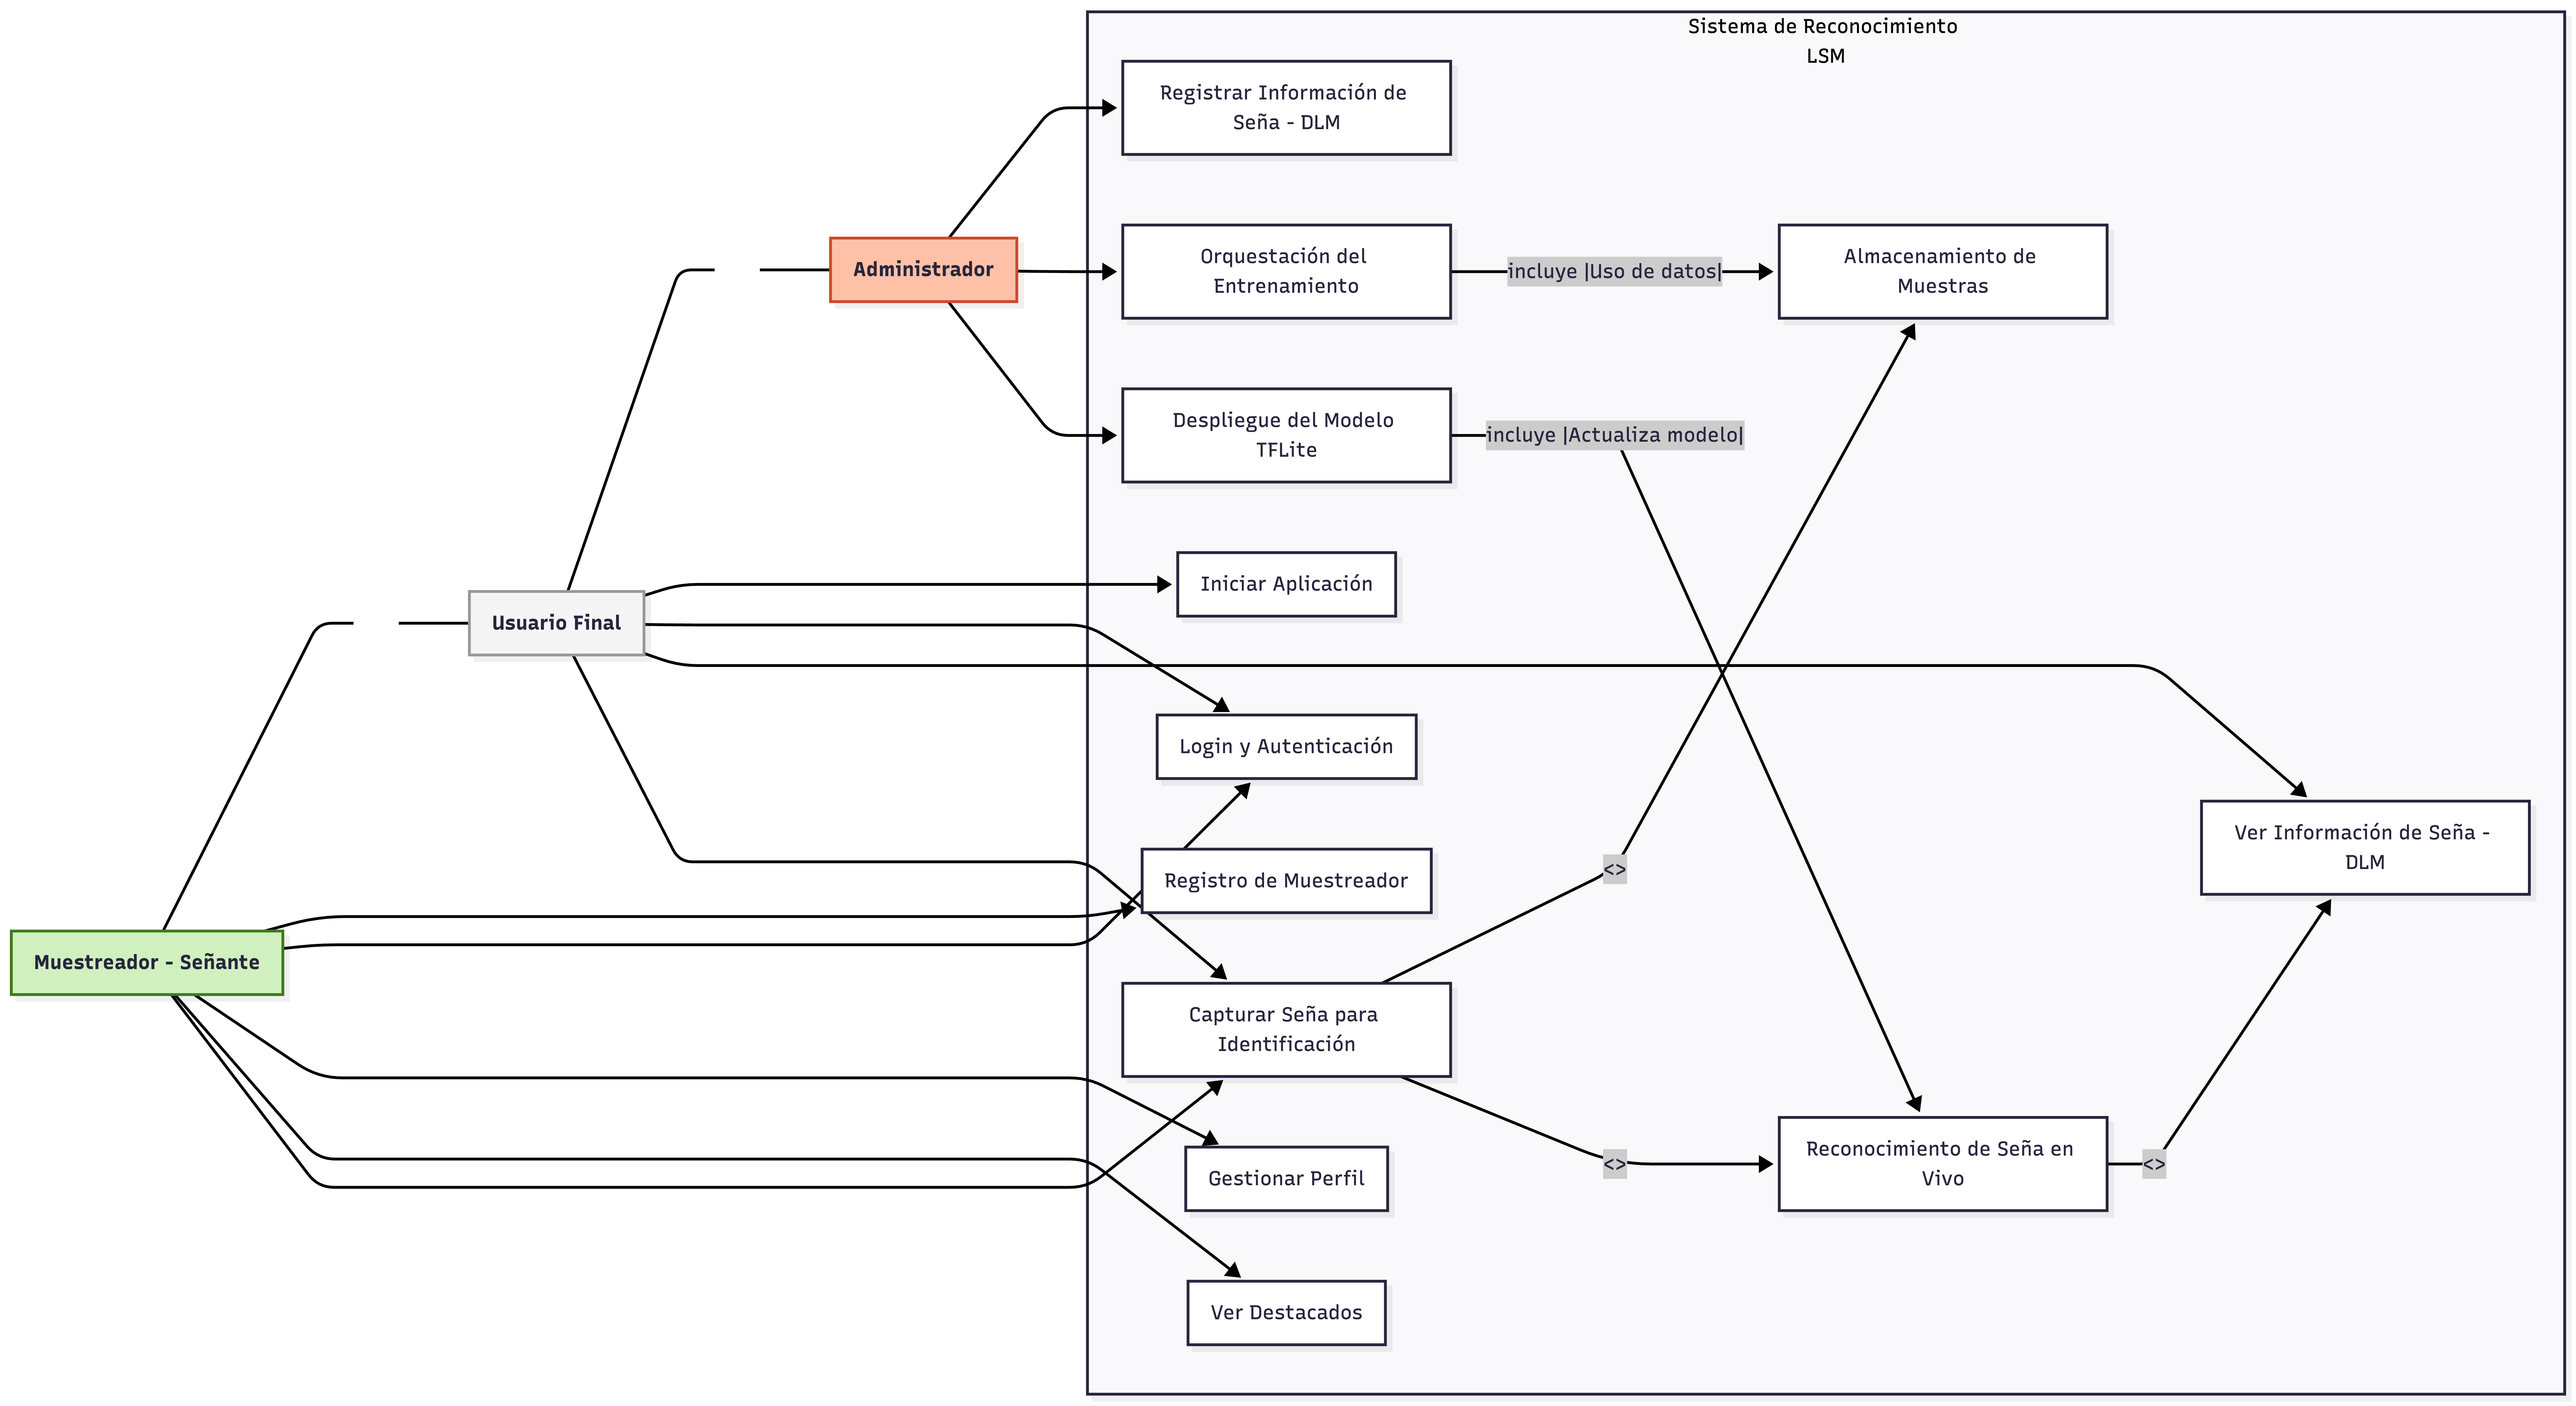
\includegraphics[width=1.2\textwidth]{CAPITULOS/capitulo4/diam}
    \caption{Diagrama de casos de uso del Sistema Principal}
    \label{fig:diagrama_casos_uso}
\end{figure}

\section{Conceptualización y Criterios del Módulo de Machine Learning} \label{sec:conceptualizacion_ml}

Para satisfacer el Requerimiento Funcional de Reconocimiento de Seña (RF08) y, especialmente, los Requerimientos No Funcionales de rendimiento (RNF01 y RNF02), se definió la arquitectura del módulo de clasificación en la fase de análisis. Este módulo se centra en la correcta interpretación de secuencias temporales de datos.

\subsection{Procesamiento de Secuencias y Arquitectura Bi-LSTM}
La Lengua de Señas Mexicana es una lengua visogestual con una fuerte dependencia del movimiento. Por ello, el algoritmo de Machine Learning debe ser capaz de procesar \textbf{secuencias de datos de longitud variable}. La decisión se centra en la justificación que sigue:

\begin{itemize}
    \item \textbf{Normalización Temporal:} Para estandarizar la duración de la seña, se implementa un \textbf{canal de progreso temporal} (ver función \texttt{\_time\_progress\_from\_ts} en \texttt{data\_processor.py}). Esta característica, añadida a los \textit{keypoints} de MediaPipe, permite al modelo Bi-LSTM aprender dónde se encuentra cada \textit{frame} dentro del ciclo de la seña (ej. inicio, articulación, final).
    \item \textbf{Arquitectura Recurrente:} Se selecciona una red \textbf{Bidirectional Long Short-Term Memory (Bi-LSTM)}, tal como se construye en \texttt{model\_constructor.py}. Esta elección es crucial, ya que permite que el modelo analice la secuencia de \textit{keypoints} tanto hacia adelante como hacia atrás, maximizando la comprensión del contexto espacial y temporal de la seña.
    \item \textbf{Técnica de Masking:} La capa \texttt{Masking} se añade en la entrada de la red para manejar secuencias de longitud variable, asegurando que los datos de relleno (\textit{padding}) sean ignorados durante el entrenamiento y la inferencia, lo cual es vital para la precisión.
\end{itemize}

\subsection{Criterios de Despliegue (Edge Computing)}
Dado el RNF02 (Latencia de < 300ms), el modelo debe ser desplegado en el dispositivo (Edge). Los criterios de diseño derivados de este requerimiento son:

\begin{enumerate}
    \item \textbf{Formato TFLite:} El modelo entrenado debe ser convertido al formato optimizado \textbf{TensorFlow Lite (TFLite)} para su ejecución eficiente en el dispositivo Android (\texttt{LiveRecognitionActivity.kt}).
    \item \textbf{Compatibilidad:} La arquitectura Bi-LSTM se construye con capas que aseguran la compatibilidad del grafo con el intérprete de TFLite, evitando operaciones complejas que no se soportan en el despliegue de borde.
\end{enumerate}

\section{Comparación de Tecnologías y Plataformas}

En esta sección se presenta un análisis comparativo integral de las principales tecnologías, plataformas y herramientas consideradas para el diseño e implementación del sistema de reconocimiento de señas. El propósito de esta comparación es evaluar, desde un punto de vista técnico y económico, las distintas alternativas disponibles en cada capa de la arquitectura, con el fin de fundamentar de manera objetiva las decisiones adoptadas en el proyecto.

El análisis abarca múltiples dimensiones del sistema, incluyendo servicios de bases de datos, opciones de cómputo (máquinas virtuales y orquestación de contenedores), almacenamiento de objetos, arquitecturas sin servidor (Function as a Service), APIs de Text-to-Speech, frameworks de aprendizaje automático, arquitecturas de redes neuronales para reconocimiento de secuencias, herramientas de infraestructura como código (IaaS), así como lenguajes y frameworks tanto para el backend como para la aplicación cliente.

Cada subsección presenta una comparación entre las soluciones más relevantes del mercado —principalmente AWS, Google Cloud y Microsoft Azure, junto con alternativas locales y frameworks de software— destacando sus ventajas, limitaciones, costos y grado de adecuación a los requerimientos específicos del proyecto. Finalmente, para cada categoría analizada, se justifica la elección de la tecnología seleccionada, asegurando coherencia arquitectónica, optimización de costos y cumplimiento de los requerimientos funcionales y de rendimiento del sistema.

\subsection{Comparación base de datos en la nube}
En la \textbf{Tabla \ref{tabla_comparativa_plataformas_nube}} se presenta una comparativa de las principales plataformas de nube consideradas para el desarrollo del proyecto, junto con las bases de datos que ofrecen, sus principales usos y su idoneidad para el procesamiento de datos de LSM.

\begin{table}[H]
    \centering
    \caption{Comparación de características entre diferentes plataformas de nube.}
    \label{tabla_comparativa_plataformas_nube}
    \begin{tabularx}{\textwidth}{|>{\raggedright\arraybackslash}p{1cm}|>{\raggedright\arraybackslash}p{2cm}|>{\raggedright\arraybackslash}X|>{\centering\arraybackslash}X|>{\raggedright\arraybackslash}X|}
        \hline
        \textbf{Nube} & \textbf{Base de datos} & \textbf{Ventajas} & \textbf{Costos} & \textbf{Principales usos} \\
        \hline
        AWS & Amazon DynamoDB &
        \begin{itemize}
            \item Amplia gama de servicios
            \item Escalabilidad
            \item Integración con servicios de IA
            \item Base de datos NoSQL
            \item Sin servidor
        \end{itemize} &
        \begin{minipage}[t]{\linewidth}
            Variable\\
            Costo total mensual: \$26.14 USD\\
            Costo por petición de lectura: \$1.05023e-08 USD\\
            Costo por petición de escritura: \$2.22412e-08 USD
        \end{minipage} &
        \begin{itemize}
            \item Cómputo
            \item Almacenamiento
            \item Machine Learning
        \end{itemize} \\
        \hline
        GCP & Cloud SQL &
        \begin{itemize}
            \item Escalabilidad
            \item Integración con TensorFlow
            \item Base de datos relacional
        \end{itemize} &
        \begin{minipage}[t]{\linewidth}
            Variable\\
            Usando MySQL \\
            Arquitectura VM \\
            db-f1-micro \\
            vCPUs: 1\\
            RAM: 3.75 GiB \\
            Costo total mensual: \$24.665 USD
        \end{minipage} &
        \begin{itemize}
            \item Big Data
            \item Machine Learning
        \end{itemize} \\
        \hline
        GCP & Firebase &
        \begin{itemize}
            \item Fácil integración con aplicaciones móviles y web
            \item Soporte para desarrollo rápido de apps
            \item Base de datos NoSQL
        \end{itemize} & Freemium &
        \begin{itemize}
            \item Desarrollo de apps móviles
            \item Desarrollo web
            \item Almacenamiento en la nube
        \end{itemize} \\
        \hline
        Azure & Azure SQL Database &
        \begin{itemize}
            \item Integración con herramientas de Microsoft
            \item Facilidad de uso
            \item Base de datos relacional
        \end{itemize} & Variable &
        \begin{itemize}
            \item Aplicaciones empresariales
            \item Bases de datos
            \item Infraestructura
        \end{itemize} \\
        \hline
    \end{tabularx}
\end{table}

\paragraph{Justificación de la Elección: Amazon DynamoDB}
es la que se ha decidió utilizar como la base de datos principal del sistema. Esta elección se basa en la necesidad de mantener una arquitectura unificada y optimizada, ya que DynamoDB es la solución NoSQL nativa de AWS, la plataforma cloud seleccionada para el despliegue de la aplicación. Su naturaleza sin servidor y su alta escalabilidad permiten una integración fluida con los demás servicios de AWS, como Lambda y S3, ofreciendo un rendimiento predecible y costos eficientes que no dependen solo del cálculo de la máquina virtual (VM), sino del consumo real de peticiones, lo cual es ideal para una aplicación con cargas de trabajo variables.

\subsection{Comparación de VM y Kubernetes de GKE}

En la \textbf{Tabla \ref{tabla_comparativa_microservicios}} se presenta una comparativa de las principales opciones de alojamiento, incluyendo Máquinas Virtuales (VM) y soluciones de contenedores gestionados (como Kubernetes de GKE, EKS y AKS), ofrecidas por las principales plataformas de nube.

\begin{table}[H]
    \centering
    \caption{Comparación de opciones para alojar microservicios en diferentes plataformas de nube.}
    \label{tabla_comparativa_microservicios}
    \begin{tabular}{|p{2.3cm}|p{1.3cm}|p{6cm}|p{6cm}|}
        \hline
        \textbf{Servicio} & \textbf{Nube} & \textbf{Ventajas} & \textbf{Costos} \\
        \hline
        Amazon EC2 & AWS &
        \begin{minipage}[t]{\linewidth}
            \begin{itemize}
                \item Variedad de tipos de instancias para diferentes cargas de trabajo
                \item Escalabilidad automática y opciones de balanceo de carga
                \item Integración con el ecosistema de AWS (RDS, S3, IAM, etc.)
            \end{itemize}
        \end{minipage} &
        % COSTOS AJUSTADOS PARA USO MÍNIMO (10 HORAS)
        \begin{minipage}[t]{\linewidth}
            Costo estimado (\textbf{Instancia Spot}): \textbf{\$10.00 - \$16.00 USD/mes} (aprox.)\\
            Costo basado en \textbf{10 horas de uso activo} de la instancia \textbf{G4dn.xlarge} (GPU):
            \begin{itemize}
                \item vCPUs: 4
                \item Memoria: 16 GiB
                \item GPU: 1 NVIDIA T4
            \end{itemize}
        \end{minipage}
        \\
        \hline
        Amazon EKS & AWS &
        \begin{minipage}[t]{\linewidth}
            \begin{itemize}
                \item Kubernetes gestionado con alta disponibilidad
                \item Fácil integración con otros servicios de AWS
            \end{itemize}
        \end{minipage} &
        \begin{minipage}[t]{\linewidth}
            Costo mensual estimado: \$365.00 USD por mes
            \begin{itemize}
                \item 1 clúster
            \end{itemize}
        \end{minipage} \\
        \hline
        Google Compute Engine (GCE) & Google Cloud &
        \begin{minipage}[t]{\linewidth}
            \begin{itemize}
                \item Alto rendimiento y opciones de personalización
                \item Escalabilidad automática y soporte de GPU/TPU
                \item Integración nativa con GKE para contenedores
            \end{itemize}
        \end{minipage} &
        \begin{minipage}[t]{\linewidth}
            Costo mensual estimado: \$5.55 USD
            \begin{itemize}
                \item Tiempo total de uso de la instancia: 730 horas/mes
                \item Sistema operativo/software: Ubuntu
                \item Tipo de máquina: f1-micro (familia de propósito general, serie N1) con 1 vCPU y 0.9 GiB de RAM
            \end{itemize}
        \end{minipage} \\
        \hline
        Google Kubernetes Engine (GKE) & Google Cloud &
        \begin{minipage}[t]{\linewidth}
            \begin{itemize}
                \item Kubernetes gestionado con escalabilidad automática
                \item Integración con el ecosistema de Google Cloud (BigQuery, Pub/Sub, etc.)
            \end{itemize}
        \end{minipage} &
        \begin{minipage}[t]{\linewidth}
            Costo Mensual estimado: \$152.55 USD
            Coste base por clúster, más recursos usados:
            \begin{itemize}
                \item Machine Family: GP Series:
                \item N1 Machine: f1-micro
            \end{itemize}
        \end{minipage} \\
        \hline
        Azure Virtual Machines & Microsoft Azure &
        \begin{minipage}[t]{\linewidth}
            \begin{itemize}
                \item Integración con otros servicios de Microsoft (Active Directory, SQL Server)
                \item Amplia variedad de opciones de instancias y series
                \item Alta disponibilidad con zonas de disponibilidad
            \end{itemize}
        \end{minipage} &
        \begin{minipage}[t]{\linewidth}
            Costo mensual estimado: \$14.60
            \begin{itemize}
                \item Instancia: A0 (1 núcleo, 0.75 GB RAM) - \$0.020/hora
                \item Sistema operativo: Windows (licencia incluida)

            \end{itemize}
        \end{minipage} \\
        \hline
        Azure Kubernetes Service (AKS) & Microsoft Azure &
        \begin{minipage}[t]{\linewidth}
            \begin{itemize}
                \item Kubernetes gestionado con integración nativa en Azure
                \item Escalabilidad automática de pods y nodos
            \end{itemize}
        \end{minipage} &
        \begin{minipage}[t]{\linewidth}
            Costo mensual estimado: \$158.41\\
            Nodos:
            \begin{itemize}
                \item Sistema operativo: Linux
                \item Instancia: D2 v3 (2 vCPUs, 8 GB RAM) - \$0.117/hora \\
            \end{itemize}

        \end{minipage} \\
        \hline
    \end{tabular}
\end{table}

\textbf{Justificación de la Elección: Amazon EC2 G4dn.xlarge (Spot)}

La elección de la instancia \textbf{Amazon EC2 G4dn.xlarge} mediante el modelo de precios \textbf{Spot} se fundamenta en los requerimientos específicos del proyecto. El \textbf{modelo de Machine Learning} basado en una arquitectura de \textbf{red neuronal recurrente (BiLSTM)} para el reconocimiento de señas requiere de una aceleración de hardware intensiva, lo cual justifica el uso de una Unidad de Procesamiento Gráfico (\textbf{GPU}).

Esta decisión técnica se sustenta en tres pilares clave:
\begin{enumerate}[label=\arabic*., nosep, itemsep=0pt]
    \item \textbf{Requerimiento de GPU:} La G4dn.xlarge proporciona una GPU NVIDIA T4, esencial para acelerar el procesamiento de \textbf{inferencia} del modelo y asegurar la baja latencia necesaria para las pruebas en tiempo real, incluso con uso esporádico.
    \item \textbf{Optimización Extrema de Costos:} Dado que el tiempo de ejecución es \textbf{extremadamente limitado (aproximadamente 10 horas al mes)}, utilizar el modelo Spot reduce el costo por hora de cómputo (GPU intensivo) a su mínima expresión. El costo mensual resultante es bajo, ya que solo cubre una pequeña fracción de horas de cómputo variable y la tarifa base fija por el \textbf{almacenamiento persistente (EBS)} de los 80 GB.
    \item \textbf{Simplicidad Arquitectónica:} La \textbf{Máquina Virtual dedicada (EC2)} simplifica la arquitectura y la gestión operativa para un uso de tan bajo volumen, evitando la complejidad y el costo base fijo de un clúster de orquestación de contenedores (EKS o GKE).
\end{enumerate}
\clearpage

\subsection{Comparación de los servicios de almacenamiento (Bucket)}
En la \textbf{Tabla \ref{tabla_comparativa_buckets}} se presenta una comparativa de las principales opciones de alojamiento de objetos (buckets) ofrecidas por las plataformas de nube.

\vspace{-0.2cm} % <--- AÑADIDO PARA REDUCIR ESPACIO VERTICAL ANTES DE LA TABLA

\begin{table}[H]
    \centering
    \caption{Comparación de servicios de almacenamiento de buckets en diferentes plataformas de nube.}
    \label{tabla_comparativa_buckets}
    \begin{tabular}{|p{1.3cm}|p{1.3cm}|p{4.5cm}|p{4.5cm}|p{4cm}|}
        \hline
        \textbf{Nube} & \textbf{Bucket} & \textbf{Ventajas} & \textbf{Costos} & \textbf{Principales usos} \\
        \hline
        AWS & Amazon S3 &
        \begin{minipage}[t]{\linewidth}
            \begin{itemize}
                \item Alta escalabilidad y durabilidad
                \item Seguridad avanzada (cifrado automático y políticas de acceso granular)
                \item Integración con servicios de AWS (Machine Learning, RedShift, etc.)
                \item Amplia documentación y soporte
            \end{itemize}
        \end{minipage} &
        \begin{minipage}[t]{\linewidth}
            \begin{itemize}
                \item \textbf{Almacenamiento:} \$115.01 USD (5 TB mensuales en S3 Standard)
                \item \textbf{S3 Select:} \$0.0028 USD (datos devueltos), \$0.008 USD (datos escaneados).
                \item \textbf{Total:} \$115.01 USD mensuales (incluyendo S3 Standard, solicitudes de datos y S3 Select).
            \end{itemize}
        \end{minipage} &
        \begin{minipage}[t]{\linewidth}
            \begin{itemize}
                \item Almacenamiento de datos y multimedia
                \item Backup y recuperación ante desastres
                \item Análisis de grandes volúmenes de datos
            \end{itemize}
        \end{minipage} \\
        \hline
        Google Cloud & Google Cloud Storage &
        \begin{minipage}[t]{\linewidth}
            \begin{itemize}
                \item Rendimiento optimizado para grandes datos
                \item Cifrado automático y opciones avanzadas de seguridad
                \item Integración con BigQuery y otras herramientas de análisis de datos
                \item Disponibilidad global con opciones de redundancia
            \end{itemize}
        \end{minipage} &
        \begin{minipage}[t]{\linewidth}
            \begin{itemize}
                \item \textbf{Almacenamiento:} \$99.90 USD (5 TB mensuales en Standard Storage).
                \item \textbf{Transferencias de datos:} Ingreso gratuito, salida desde \$0.12/GB.
                \item \textbf{Operaciones:} \$0.005 por 10,000 operaciones de clase A.
            \end{itemize}
        \end{minipage} &
        \begin{minipage}[t]{\linewidth}
            \begin{itemize}
                \item Almacenamiento de datos
                \item Entrenamiento de modelos de Machine Learning
                \item Archivado y recuperación
                \item Análisis de grandes volúmenes de datos
            \end{itemize}
        \end{minipage} \\
        \hline
        Microsoft Azure & Azure Blob Storage &
        \begin{minipage}[t]{\linewidth}
            \begin{itemize}
                \item Integración con ecosistema de Microsoft (Office, Power BI, etc.)
                \item Escalabilidad con opciones de redundancia (LRS, GRS)
                \item Seguridad con cifrado en tránsito y en reposo
                \item Soporte para migraciones híbridas (Azure Arc)
            \end{itemize}
        \end{minipage} &
        \begin{minipage}[t]{\linewidth}
            \begin{itemize}
                \item \textbf{Standard (GPv2):} Hot (\$0.018/GB), Cool (\$0.01/GB), Archive (\$0.002/GB).
                \item \textbf{Premium:} Optimizado para baja latencia, \$0.15/GB.
                \item \textbf{Reservado:} 100 TB (1 año, \$1,545 Hot), 1 PB (1 año, \$15,050).
                \item \textbf{Early Deletion Penalty:} 30 días (Cool), 90 días (Cold), 180 días (Archive).
            \end{itemize}
        \end{minipage} &
        \begin{minipage}[t]{\linewidth}
            \begin{itemize}
                \item Almacenamiento de datos no estructurados
                \item Respaldo y recuperación ante desastres
                \item Analítica avanzada
                \item Archivo de documentos y multimedia
            \end{itemize}
        \end{minipage} \\
        \hline
    \end{tabular}
\end{table}

\paragraph{Justificación de la Elección: Amazon Simple Storage Service (S3)}
Se ha seleccionado \textbf{Amazon S3} como el servicio de almacenamiento de objetos central del sistema. Esta elección se basa principalmente en la necesidad de integración nativa con la infraestructura AWS ya establecida (EC2 y DynamoDB), y la naturaleza crítica de los datos almacenados. S3 será utilizado para almacenar los siguientes activos:

\begin{enumerate}[label=\arabic*., nosep, itemsep=0pt]
    \item \textbf{Datos Crudos del Modelo (CSV de Keypoints):} Los archivos CSV que contienen las secuencias temporales de Keypoints, que son la materia prima para el entrenamiento y la inferencia del modelo BiLSTM, requieren la \textbf{durabilidad de 99.999999999\%} que ofrece S3 Standard para garantizar la integridad y persistencia de los datos del proyecto.
    \item \textbf{Modelo Compilado:} El archivo del modelo de red neuronal entrenado debe estar disponible con alta fiabilidad para ser cargado por la instancia EC2 (\textbf{G4dn.xlarge}), beneficiándose de la baja latencia de acceso.
    \item \textbf{Archivos de Perfil de Usuario:} Incluyendo fotos de perfil y otros archivos no estructurados que requieran seguridad y fácil gestión de acceso.
\end{enumerate}

La integración nativa de S3 con AWS IAM (para políticas de seguridad) y la facilidad de conexión con la capa de cómputo hacen de esta opción la más eficiente y coherente para la arquitectura del proyecto.

\subsection{Comparación de Function as a Service (FaaS)}

En la \textbf{Tabla \ref{tabla_comparativa_faas}} se presenta una comparativa de los servicios de Function as a Service (FaaS) en las principales plataformas de nube, incluyendo el modelo de costos basado en el consumo.

\begin{table}[H]
    \centering
    \caption{Comparación de Function as a Service en diferentes plataformas de nube.}
    \label{tabla_comparativa_faas}
    \begin{tabular}{|p{1.5cm}|p{1.5cm}|p{4.5cm}|p{5cm}|p{3cm}|} % Se ajustaron los anchos de columna
        \hline
        \textbf{Nube} & \textbf{FaaS} & \textbf{Ventajas} & \textbf{Costo Estimado (por 1 millón de peticiones)} & \textbf{Lenguajes Soportados} \\
        \hline
        AWS & AWS Lambda &
        \begin{minipage}[t]{\linewidth}
            \begin{itemize}
                \item Escalabilidad automática
                \item Integración nativa con DynamoDB, S3 y API Gateway.
                \item Pago por uso.
            \end{itemize}
        \end{minipage} &
        \begin{minipage}[t]{\linewidth}
            \textbf{Aprox. \$2.00 - \$4.00 USD} (Cálculo basado en solicitudes y GB-segundos, posterior a la capa gratuita).
        \end{minipage} &
        \begin{minipage}[t]{\linewidth}
            \begin{itemize}
                \item Python, Node.js, Java, Ruby
            \end{itemize}
        \end{minipage} \\
        \hline
        Google Cloud & Cloud Functions &
        \begin{minipage}[t]{\linewidth}
            \begin{itemize}
                \item Escalabilidad y seguridad
                \item Integración con Google Cloud
            \end{itemize}
        \end{minipage} &
        \begin{minipage}[t]{\linewidth}
            \textbf{Aprox. \$2.50 - \$4.50 USD} (Similar a AWS, posterior a la capa gratuita).
        \end{minipage} &
        \begin{minipage}[t]{\linewidth}
            \begin{itemize}
                \item Node.js, Python, Go
            \end{itemize}
        \end{minipage} \\
        \hline
        Microsoft Azure & Azure Functions &
        \begin{minipage}[t]{\linewidth}
            \begin{itemize}
                \item Integración con servicios de Microsoft
                \item Buen soporte para CI/CD
            \end{itemize}
        \end{minipage} &
        \begin{minipage}[t]{\linewidth}
            \textbf{Aprox. \$2.20 - \$4.20 USD} (Basado en el plan de consumo, posterior a la capa gratuita).
        \end{minipage} &
        \begin{minipage}[t]{\linewidth}
            \begin{itemize}
                \item C\#, JavaScript, Python, Java
            \end{itemize}
        \end{minipage} \\
        \hline
    \end{tabular}
\end{table}

\paragraph{Justificación de la Elección: AWS Lambda}
La selección de \textbf{AWS Lambda} se alinea con la estrategia de mantener una arquitectura de nube unificada en AWS (junto a DynamoDB, S3 y EC2). Lambda es la elección óptima para desacoplar y orquestar las tareas del backend sin incurrir en costos de cómputo inactivos, con un \textbf{costo marginal por petición muy bajo} una vez agotada la generosa capa gratuita.

El diseño del sistema requiere la implementación de \textbf{cuatro funciones Lambda} distintas para manejar responsabilidades específicas, asegurando la escalabilidad e independencia de cada proceso:

\begin{enumerate}[label=\arabic*., nosep, itemsep=0pt]
    \item \textbf{Gestión de Autenticación/Usuarios:} Manejo de registro, inicio de sesión y validación de tokens de usuario.
    \item \textbf{Control de Datos LSM:} Interacción directa con \textbf{DynamoDB} para consultar y almacenar información de la base de datos (metadatos de las señas y perfiles).
    \item \textbf{Gestión de Archivos (S3 Trigger):} Activada por eventos de \textbf{S3}, como la subida de una nueva foto de perfil o un archivo CSV de entrenamiento, gestionando el acceso y la notificación.
    \item \textbf{Orquestación de la Inferencia (EC2 Trigger):} Encargada de comunicarse con la instancia \textbf{EC2 G4dn.xlarge} para iniciar el proceso de inferencia del modelo BiLSTM cuando se recibe una solicitud de reconocimiento de seña.
\end{enumerate}

Este enfoque permite que cada componente del backend escale de forma independiente, pagando únicamente por los milisegundos de cómputo utilizados por cada una de las cuatro funciones.

\subsection{Comparación de APIs de Text-to-Speech (TTS)}

En la \textbf{Tabla \ref{tabla_comparativa_tts}} se presenta una comparativa de las APIs de Text-to-Speech (TTS) en las principales plataformas de nube y la solución nativa de Android.

\begin{table}[H]
    \centering
    \caption{Comparación de servicios Text-to-Speech (TTS): Soluciones en la nube vs. Solución nativa.}
    \label{tabla_comparativa_tts}
    \begin{tabular}{|p{2.5cm}|p{3cm}|p{4cm}|p{3cm}|p{3cm}|}
        \hline
        \textbf{Plataforma} & \textbf{API de TTS} & \textbf{Características} & \textbf{Idiomas soportados} & \textbf{Costo Estimado} \\
        \hline
        AWS & Amazon Polly &
        \begin{minipage}[t]{\linewidth}
            \begin{itemize}
                \item Voces naturales (Neural TTS)
                \item Opciones de personalización
                \item Soporte SSML
            \end{itemize}
        \end{minipage} &
        Más de 30 &
        \begin{minipage}[t]{\linewidth}
            \textbf{Aprox. \$4.00 USD} por 1 millón de caracteres (TTS Estándar)
        \end{minipage} \\
        \hline
        Google Cloud & Google Text-to-Speech &
        \begin{minipage}[t]{\linewidth}
            \begin{itemize}
                \item Tecnología WaveNet
                \item Personalización con SSML
            \end{itemize}
        \end{minipage} &
        Más de 30 &
        \begin{minipage}[t]{\linewidth}
            \textbf{Aprox. \$4.00 USD} por 1 millón de caracteres (TTS Estándar)
        \end{minipage} \\
        \hline
        Microsoft Azure & Azure Speech &
        \begin{minipage}[t]{\linewidth}
            \begin{itemize}
                \item Soporte de voz neural
                \item Personalización de tonos
            \end{itemize}
        \end{minipage} &
        Más de 40 &
        \begin{minipage}[t]{\linewidth}
            \textbf{Aprox. \$4.00 USD} por 1 millón de caracteres (TTS Estándar)
        \end{minipage} \\
        \hline
        Android Nativo & TextToSpeech &
        \begin{minipage}[t]{\linewidth}
            \begin{itemize}
                \item Ejecución local (client-side)
                \item Latencia mínima (sin red)
                \item Funcionalidad offline
            \end{itemize}
        \end{minipage} &
        Depende del dispositivo &
        \begin{minipage}[t]{\linewidth}
            \textbf{Costo de uso nulo} (Gratuito)
        \end{minipage} \\
        \hline
    \end{tabular}
\end{table}

\paragraph{Justificación de la Elección: API Nativa de Android (TextToSpeech)}
Para la funcionalidad de respuesta de voz, el sistema ha optado por utilizar la API nativa de Android, `android.speech.tts.TextToSpeech`, en lugar de las soluciones basadas en la nube. Esta decisión se fundamenta en la arquitectura client-side (del lado del cliente) de la aplicación y en la optimización de recursos y costos:

\begin{enumerate}[label=\arabic*., nosep, itemsep=0pt]
    \item \textbf{Costo Cero (Free Tier):} El uso de la API nativa de Android no genera costos de transacción, consumo de caracteres o latencia de red, a diferencia de las APIs de nube que, aunque tienen una capa gratuita, comienzan a incurrir en gastos con el aumento de uso.
    \item \textbf{Latencia y Rendimiento:} Al ejecutar la síntesis de voz directamente en el dispositivo (cliente), se elimina la latencia de red asociada con el envío de texto a la nube y la recepción del audio.
\end{enumerate}

\subsection{Comparación de Frameworks de Aprendizaje Automático para Reconocimiento}

En la \textbf{Tabla \ref{tabla_comparativa_frameworks}} se presenta una comparativa de los frameworks de aprendizaje automático más utilizados en tareas de reconocimiento de secuencias y visión.

\begin{table}[H]
    \centering
    \caption{Comparación de frameworks de aprendizaje automático para reconocimiento de secuencias.}
    \label{tabla_comparativa_frameworks}
    \begin{tabular}{|p{1.8cm}|p{2.5cm}|p{6.5cm}|p{5cm}|} % Ajuste de anchos para optimizar el espacio
        \hline
        \textbf{Framework} & \textbf{Compatibilidad} & \textbf{Ventajas} & \textbf{Ecosistema y Uso Típico} \\
        \hline
        TensorFlow &
        Multiplataforma (Linux, macOS, Windows) y móvil (Lite) &
        \begin{itemize}
            \item Amplia comunidad, soporte y madurez industrial.
            \item Alto rendimiento en producción y despliegue masivo.
            \item Arquitectura flexible (gráficos estáticos).
        \end{itemize} &
        \begin{itemize}
            \item Modelado de series temporales (RNN, LSTM).
            \item Despliegue en producción (TF Serving, Lite).
        \end{itemize} \\
        \hline
        Keras &
        API de alto nivel para TensorFlow, PyTorch y Theano &
        \begin{itemize}
            \item Simplificación del desarrollo de redes neuronales (fácil y rápido).
            \item Enfocado en la usabilidad y prototipado rápido.
            \item Interfaz estandarizada e intuitiva.
        \end{itemize} &
        \begin{itemize}
            \item Prototipado y desarrollo de Deep Learning.
            \item Construcción de modelos LSTM y BiLSTM.
        \end{itemize} \\
        \hline
        PyTorch &
        Multiplataforma y soporte nativo para GPUs de Nvidia &
        \begin{itemize}
            \item Modelo de grafo dinámico (fácil de depurar y flexible).
            \item Amplio uso en investigación y desarrollo de algoritmos de vanguardia.
            \item Orientado a objetos y muy pitónico.
        \end{itemize} &
        \begin{itemize}
            \item Reconocimiento de voz y clasificación de imágenes.
            \item Investigación y desarrollo de modelos nuevos.
        \end{itemize} \\
        \hline
        MediaPipe &
        C++, Python, JavaScript (Web), Android, iOS &
        \begin{itemize}
            \item Toolkit especializado en percepción multiplataforma.
            \item Detección eficiente de keypoints 3D de Pose, Manos y Rostro.
            \item Optimizado para aplicaciones en tiempo real y on-device.
        \end{itemize} &
        \begin{itemize}
            \item Extracción de características (Preprocesamiento).
            \item Seguimiento y reconocimiento de gestos.
        \end{itemize} \\
        \hline
        OpenCV &
        Multiplataforma; C++ y Python &
        \begin{itemize}
            \item Biblioteca extensa de algoritmos de visión clásica.
            \item Ideal para aplicaciones en tiempo real.
            \item Compatibilidad con C++ y Python.
        \end{itemize} &
        \begin{itemize}
            \item Detección y seguimiento de objetos.
            \item Manipulación de píxeles (pre-procesamiento de video).
        \end{itemize} \\
        \hline
    \end{tabular}
\end{table}

\paragraph{Justificación de la Elección: Keras, TensorFlow y MediaPipe}
La arquitectura de software se basa en la API de \textbf{Keras} con \textbf{TensorFlow} como backend para el modelo BiLSTM, utilizando \textbf{MediaPipe} como herramienta de extracción de características. Esta decisión estratégica se justifica por:

\begin{enumerate}[label=\arabic*., nosep, itemsep=0pt]
    \item \textbf{Eficiencia en Desarrollo (Keras):} La API de Keras simplifica drásticamente la construcción y el entrenamiento de la arquitectura \textbf{Deep BiLSTM}, reduciendo la complejidad del código y el tiempo de prototipado. Keras permite enfocarse en la estructura del modelo sin manejar el detalle de las operaciones de bajo nivel del grafo.
    \item \textbf{Integración y Despliegue (TensorFlow):} Al utilizar TensorFlow como backend, el modelo se beneficia de un ecosistema maduro y enfocado en la producción. Esto facilita el proceso de guardar el modelo en formatos optimizados para el despliegue y su posterior carga en la instancia \textbf{EC2 G4dn.xlarge} para la fase de inferencia en producción.
    \item \textbf{Herramienta de Entrada (MediaPipe):} La elección de \textbf{MediaPipe} es fundamental, ya que es la única biblioteca capaz de proporcionar de manera eficiente los \textbf{vectores de 195 dimensiones (Keypoints de Pose y Manos)} necesarios como entrada secuencial para el modelo BiLSTM. MediaPipe actúa como la capa de extracción de características críticas para el modelo.
\end{enumerate}
\clearpage

\subsection{Comparación de Arquitecturas para el Reconocimiento de Secuencias}

En la \textbf{Tabla \ref{tabla_comparativa_algoritmos}} se presenta una comparación enfocada en redes neuronales profundas, destacando la evolución hacia la arquitectura seleccionada para este proyecto.

\begin{table}[H]
    \centering
    \caption{Comparación de arquitecturas de aprendizaje profundo para el reconocimiento de gestos y secuencias (LSM).}
    \label{tabla_comparativa_algoritmos}
    \begin{tabular}{|p{2.5cm}|p{4.5cm}|p{4.5cm}|p{4.5cm}|}
        \hline
        \textbf{Arquitectura} & \textbf{Características Principales} & \textbf{Aplicación en Video/Señas} & \textbf{Relevancia para el Proyecto} \\
        \hline
        \textbf{CNN} \newline (Redes Neuronales Convolucionales) &
        \begin{itemize}
            \item Especializadas en procesar datos tipo rejilla (imágenes).
            \item Extraen características \textbf{espaciales} (formas de manos, posición del cuerpo).
        \end{itemize} &
        \begin{itemize}
            \item Base de herramientas como \textit{MediaPipe}.
            \item Procesan cada fotograma de forma individual, sin memoria del pasado.
        \end{itemize} &
        \begin{itemize}
            \item Se utilizan implícitamente en la fase de extracción de características (\textbf{MediaPipe}), pero por sí solas no capturan el movimiento temporal de la seña.
        \end{itemize} \\
        \hline
        \textbf{LSTM} \newline (Long Short-Term Memory) &
        \begin{itemize}
            \item Redes recurrentes con "celdas de memoria" para retener información a largo plazo.
            \item Solucionan el problema de desvanecimiento de gradiente de las RNN simples.
        \end{itemize} &
        \begin{itemize}
            \item Ideales para datos secuenciales (series de tiempo, texto, video).
            \item Analizan el movimiento basándose solo en lo ocurrido en el pasado ($t-1$).
        \end{itemize} &
        \begin{itemize}
            \item Son capaces de aprender la secuencia de una seña, pero tienen limitaciones al no conocer el contexto futuro del gesto en movimientos complejos.
        \end{itemize} \\
        \hline
        \textbf{BiLSTM} \newline (Bidirectional LSTM) &
        \begin{itemize}
            \item \textbf{Arquitectura seleccionada.}
            \item Entrena dos capas LSTM simultáneas: una procesa la secuencia de inicio a fin (Forward) y otra de fin a inicio (Backward).
        \end{itemize} &
        \begin{itemize}
            \item Captura el contexto completo de la secuencia.
            \item Crucial en LSM donde la intención de un movimiento inicial a menudo se clarifica por cómo termina la seña.
        \end{itemize} &
        \begin{itemize}
            \item \textbf{Elección del sistema:} Proporciona la mayor precisión al entender la "coarticulación" de los gestos.
            \item Permite distinguir señas con movimientos similares pero contextos diferentes.
        \end{itemize} \\
        \hline
    \end{tabular}
\end{table}

\paragraph{Justificación de la Elección: Arquitectura Bidirectional LSTM (BiLSTM)}
La arquitectura \textbf{BiLSTM} fue seleccionada como la columna vertebral del modelo de reconocimiento de señas por su superioridad inherente en el manejo de datos secuenciales con dependencia de contexto. Esta justificación se basa en tres puntos clave:

\begin{enumerate}[label=\arabic*., nosep, itemsep=0pt]
    \item \textbf{Captura de Contexto Completo:} A diferencia de la LSTM simple, la BiLSTM procesa la secuencia de \textbf{Keypoints} de dos formas: del inicio al final y del final al inicio. Esto es crucial en la Lengua de Señas Mexicana (LSM), donde el significado de un movimiento inicial (e.g., subir la mano) puede depender de la forma en que el gesto concluye. La BiLSTM tiene acceso a ese contexto "futuro" durante el entrenamiento, mejorando drásticamente la precisión.
    \item \textbf{Manejo de Coarticulación:} La capacidad bidireccional permite a la red modelar la coarticulación de los gestos, es decir, cómo el movimiento de una seña influye o se anticipa al movimiento de la seña siguiente. Esto permite distinguir señas con movimientos muy similares pero con transiciones o terminaciones diferentes.
    \item \textbf{Separación de Responsabilidades (CNN vs. BiLSTM):} Es fundamental notar que el sistema divide las tareas:
    \begin{itemize}[nosep, itemsep=0pt] % Aquí se ajusta el espaciado
        \item Las \textbf{CNN} (a través de \textbf{MediaPipe}) son responsables de la extracción de características espaciales (Keypoints) en cada fotograma.
        \item La \textbf{BiLSTM} es responsable de analizar la \textbf{dimensión temporal} de esos Keypoints a lo largo de la secuencia de tiempo, lo que constituye la verdadera tarea de reconocimiento de la seña.
    \end{itemize}
\end{enumerate}
Este enfoque garantiza que el modelo utilice la herramienta más avanzada para cada fase del procesamiento, optimizando la precisión del sistema final.
\clearpage

\subsection{Comparación de lenguajes y frameworks para IaaS}

En la Tabla \ref{tabla_comparativa_iaas} se presenta una comparativa de los principales lenguajes y frameworks utilizados para la gestión de infraestructura como servicio (IaaS), como AWS CloudFormation, Terraform y el marco de trabajo Serverless Application Model (SAM). Estos frameworks permiten la automatización de la infraestructura en la nube, facilitando la creación, configuración y despliegue de recursos de manera eficiente y escalable.

\begin{table}[H]
    \centering
    \caption{Comparación de lenguajes y frameworks para la gestión de infraestructura como servicio (IaaS).}
    \label{tabla_comparativa_iaas}
    \begin{tabular}{|p{2cm}|p{4.5cm}|p{4cm}|p{4cm}|}
        \hline
        \textbf{Framework / Lenguaje} & \textbf{Plataforma Compatible} & \textbf{Ventajas} & \textbf{Principales Usos} \\
        \hline
        AWS CloudFormation &
        AWS &
        \begin{minipage}[t]{\linewidth}
            \begin{itemize}
                \item Integración nativa con AWS.
                \item Soporte para la gestión de recursos complejos.
                \item Escalabilidad y automatización de infraestructuras.
            \end{itemize}
        \end{minipage} &
        \begin{minipage}[t]{\linewidth}
            \begin{itemize}
                \item Despliegue de infraestructuras completas en AWS.
                \item Gestión de entornos de producción, desarrollo y prueba.
                \item Creación de pilas de recursos (stacks) en AWS.
            \end{itemize}
        \end{minipage} \\
        \hline
        Terraform &
        Multicloud (AWS, Azure, Google Cloud, entre otros) &
        \begin{minipage}[t]{\linewidth}
            \begin{itemize}
                \item Multicloud (compatible con múltiples proveedores).
                \item Declarativo y con amplio soporte de proveedores de nube.
                \item Gestión de infraestructura como código (IaC).
            \end{itemize}
        \end{minipage} &
        \begin{minipage}[t]{\linewidth}
            \begin{itemize}
                \item Gestión de infraestructuras en entornos multicloud.
                \item Definición de infraestructura como código para automatizar el aprovisionamiento.
                \item Creación y mantenimiento de entornos a través de archivos de configuración.
            \end{itemize}
        \end{minipage} \\
        \hline
        AWS SAM (Serverless Application Model) &
        AWS (específicamente para aplicaciones sin servidor) &
        \begin{minipage}[t]{\linewidth}
            \begin{itemize}
                \item Simplificación de aplicaciones sin servidor en AWS.
                \item Integración directa con AWS Lambda y otros servicios sin servidor.
                \item Simplificación del proceso de despliegue con plantillas.
            \end{itemize}
        \end{minipage} &
        \begin{minipage}[t]{\linewidth}
            \begin{itemize}
                \item Despliegue de aplicaciones sin servidor (serverless) en AWS.
                \item Integración de funciones Lambda, API Gateway y DynamoDB.
                \item Simplificación de la gestión de recursos sin servidor y microservicios.
            \end{itemize}
        \end{minipage} \\
        \hline
    \end{tabular}
\end{table}

\paragraph{Justificación de la Elección: AWS CloudFormation}

La elección de \textbf{AWS CloudFormation} como framework principal para la gestión de infraestructura como servicio (IaaS) se fundamenta en su capacidad para proporcionar un control exhaustivo y nativo sobre el ciclo de vida de los recursos dentro de la nube de Amazon Web Services (AWS). Aunque alternativas como Terraform ofrecen un enfoque multicloud y AWS SAM simplifica el serverless, CloudFormation se alinea mejor con los requisitos de un sistema robusto y centrado exclusivamente en AWS, por las siguientes razones:

\begin{enumerate}[label=\arabic*., nosep, itemsep=0pt]
    \item \textbf{Integración Nativa y Profunda:} Al ser una herramienta nativa de AWS, CloudFormation garantiza una integración de primer nivel con todos los servicios de AWS, incluyendo los más recientes y complejos. Esto minimiza los posibles retrasos o incompatibilidades que pueden surgir con herramientas de terceros (como Terraform) al gestionar servicios específicos de AWS.
    \item \textbf{Gestión de Ciclo de Vida del Stack:} Permite manejar colecciones de recursos (denominadas stacks) como una única unidad. Esta característica es vital para entornos de producción y prueba, ya que asegura que la creación, actualización o eliminación de la infraestructura se realice de manera atómica, garantizando la consistencia y reduciendo el riesgo de dejar recursos huérfanos o en estados inconsistentes.
    \item \textbf{Seguridad y Gobernanza:} Las plantillas de CloudFormation se validan y procesan a través de los mecanismos de AWS, lo que facilita la implementación de políticas de seguridad y cumplimiento normativo. La creación de Change Sets permite previsualizar exactamente qué recursos serán modificados antes de aplicar los cambios a la infraestructura, ofreciendo una capa crítica de seguridad operacional.
    \item \textbf{Control de Costos:} Al ser una herramienta declarativa y nativa, CloudFormation proporciona una visión clara de los recursos desplegados dentro de un stack, lo cual es fundamental para el monitoreo y la optimización de costos en la plataforma AWS.
\end{enumerate}

Este enfoque nativo proporciona la estabilidad, el control y la escalabilidad necesarias para gestionar eficientemente la infraestructura que soporta la aplicación de reconocimiento de secuencias.

\clearpage

\subsection{Lenguajes de Programación para el Backend}

Para el desarrollo del backend, se ha optado por un enfoque híbrido que aprovecha las fortalezas de dos lenguajes de programación principales: Python y JavaScript (Node.js). Esta estrategia permite optimizar el rendimiento y la eficiencia de costos en la arquitectura de microservicios de AWS. En la \textbf{Tabla \ref{tabla_comparativa_backend}} se presenta una comparación de los lenguajes de programación considerados para el desarrollo de los microservicios en AWS. Esta comparación es crucial para determinar la distribución de responsabilidades, decidiendo qué lenguaje es más eficiente para el cómputo intensivo del modelo BiLSTM y cuál es mejor para la orquestación del servidor.

\begin{table}[H]
    \centering
    \caption{Comparación de Lenguajes de Programación para Microservicios y Lógica de Negocio (Backend).}
    \label{tabla_comparativa_backend}
    \begin{tabular}{|p{1.8cm}|p{3.5cm}|p{5cm}|p{6cm}|}
        \hline
        \textbf{Lenguaje} & \textbf{Rol en el Proyecto} & \textbf{Ventajas Clave} & \textbf{Relevancia para el Proyecto} \\
        \hline
        \textbf{Python} &
        Lógica del \textbf{Modelo BiLSTM}, Preprocesamiento y Tareas Pesadas (EC2/Lambda) &
        \begin{itemize}[nosep, itemsep=0pt]
            \item Ecosistema robusto de ML (TensorFlow/Keras).
            \item Rapidez de prototipado y depuración.
            \item Legibilidad óptima para manipulación de datos.
        \end{itemize} &
        \textbf{Elegido para el cómputo de inferencia}, ya que simplifica la integración directa con las librerías de Deep Learning, siendo el estándar de la industria. \\
        \hline
        \textbf{JavaScript} \newline (Node.js) &
        Servicios de API Gateway, Enrutamiento y Lógica de Negocio (Lambda/Serverless) &
        \begin{itemize}[nosep, itemsep=0pt]
            \item Alto rendimiento en operaciones I/O (asíncrono).
            \item Ecosistema nativo para AWS Serverless (rápida inicialización).
            \item Curva de aprendizaje baja.
        \end{itemize} &
        \textbf{Elegido para la capa de microservicios}, ofreciendo velocidad y eficiencia en el manejo de peticiones web y la comunicación asíncrona. \\
        \hline
        \textbf{Go (Golang)} &
        Servicios de Alto Rendimiento / Alternativa Serverless &
        \begin{itemize}[nosep, itemsep=0pt]
            \item Lenguaje compilado, alta velocidad y eficiencia en uso de memoria.
            \item Excelente manejo de la concurrencia.
            \item Despliegue de binarios pequeños.
        \end{itemize} &
        \textbf{Descartado:} Aunque es rápido, su ecosistema de Deep Learning es inmaduro comparado con Python, lo que complicaría la integración y el mantenimiento del modelo BiLSTM. \\
        \hline
    \end{tabular}
\end{table}

\paragraph{Justificación del Enfoque Híbrido en el Backend}
La arquitectura de backend utiliza una doble capa para optimizar los recursos. \textbf{JavaScript} se encarga del manejo rápido y asíncrono de las peticiones del \textbf{API Gateway} y la lógica serverless de bajo cómputo, actuando como un orquestador eficiente. Por otro lado, \textbf{Python} es el lenguaje exclusivo para las funciones críticas de \textbf{inferencia del modelo BiLSTM}, garantizando la máxima compatibilidad y rendimiento con las librerías de TensorFlow/Keras. Esta división asegura que cada lenguaje se use para la tarea en la que sobresale, maximizando la eficiencia operativa.

\subsection{Lenguajes de Programación para la Aplicación Cliente}

El desarrollo de la aplicación móvil requiere un lenguaje que asegure el máximo rendimiento y una baja latencia en tareas intensivas como la captura y el procesamiento de video con MediaPipe. En la \textbf{Tabla \ref{tabla_comparativa_client_app}} se analizan las opciones para el desarrollo de la aplicación móvil cliente. La elección se centra en garantizar el máximo rendimiento para las tareas intensivas de video y cámara que requiere la integración con MediaPipe.

\begin{table}[H]
    \centering
    \caption{Comparación de Lenguajes y Frameworks para el Desarrollo de Aplicaciones Cliente.}
    \label{tabla_comparativa_client_app}
    \begin{tabular}{|p{2.5cm}|p{3.5cm}|p{5cm}|p{5.5cm}|}
        \hline
        \textbf{Lenguaje} & \textbf{Plataforma de Despliegue} & \textbf{Ventajas Clave} & \textbf{Desventajas y Decisión} \\
        \hline
        \textbf{Kotlin} &
        Android Nativo / KMM (Multiplataforma) &
        \begin{itemize}[nosep, itemsep=0pt]
            \item Lenguaje moderno, conciso y seguro (minimiza errores de null).
            \item \textbf{Soporte oficial de Google} para el desarrollo de Android.
            \item Excelente interoperabilidad con Java.
        \end{itemize} &
        \textbf{Elección del Cliente:} Proporciona el \textbf{mejor rendimiento nativo} en aplicaciones Android, crucial para el procesamiento en tiempo real de la cámara y la integración eficiente de la capa de MediaPipe. \\
        \hline
        \textbf{Java} &
        Android Nativo (Tradicional) &
        \begin{itemize}[nosep, itemsep=0pt]
            \item Amplia base de código legado y documentación.
            \item Alto rendimiento nativo.
        \end{itemize} &
        Es una alternativa viable, pero el lenguaje es más verboso, requiere más código para las mismas funcionalidades y es menos seguro que Kotlin, lo que aumenta el tiempo de desarrollo. \\
        \hline
        \textbf{React Native} &
        iOS / Android (Híbrido) &
        \begin{itemize}[nosep, itemsep=0pt]
            \item Una sola base de código para ambas plataformas.
            \item Amplia comunidad web.
        \end{itemize} &
        \textbf{Descartado:} No es adecuado debido a la necesidad de rendimiento \textbf{nativo puro} para tareas intensivas como la integración profunda de la cámara y la latencia en el procesamiento de Keypoints, donde las capas puente pueden ser limitantes. \\
        \hline
    \end{tabular}
\end{table}

\paragraph{Justificación de la Elección de Kotlin}
Se seleccionó \textbf{Kotlin} como lenguaje principal para la aplicación cliente debido a que es el estándar moderno y oficialmente preferido por Google para el desarrollo de Android. Esta elección asegura una integración de máximo rendimiento con las APIs del sistema operativo y las librerías nativas de la cámara, un requisito indispensable para la baja latencia exigida por el procesamiento de \textbf{MediaPipe} y la comunicación eficiente con el \textbf{API Gateway} del backend. Esto garantiza una experiencia de usuario fluida y receptiva.

\subsection{Tecnologías Utilizadas}

A continuación, se detallan las principales tecnologías que serán utilizadas para el desarrollo, entrenamiento y despliegue del sistema de reconocimiento de LSM, alineadas con la arquitectura BiLSTM y la infraestructura AWS.

\begin{itemize}[nosep, itemsep=0.7pt]
    \item \textbf{Herramientas Core y Modelado}
    \begin{itemize}[nosep, itemsep=0pt]
        \item \textbf{Python}: Lenguaje de programación principal para la lógica del sistema, pre-procesamiento de datos y el flujo de trabajo de aprendizaje profundo.
        \item \textbf{MediaPipe Holistic}: Módulo clave para la extracción de características espaciales (Keypoints de manos, cuerpo y rostro) en tiempo real, proporcionando las secuencias de entrada para la red BiLSTM.
        \item \textbf{TensorFlow / Keras}: Framework principal de Deep Learning utilizado para construir, entrenar y optimizar la arquitectura de red Bidirectional LSTM (BiLSTM), responsable del análisis de la dimensión temporal.
    \end{itemize}

    \item \textbf{Arquitectura Cloud y Microservicios (AWS)}
    \begin{itemize}[nosep, itemsep=0pt]
        \item \textbf{Amazon API Gateway}: Actúa como el \textbf{punto de entrada unificado} para la interfaz web. Recibe las peticiones de reconocimiento y las enruta a las funciones Lambda correspondientes.
        \item \textbf{AWS Lambda}: Ejecuta el código de inferencia del modelo BiLSTM en un entorno serverless, escalable y bajo demanda, lo cual optimiza los costos operativos.
        \item \textbf{Amazon S3 (Simple Storage Service)}: Almacenamiento escalable de objetos para videos fuente, secuencias de Keypoints pre-procesados y los modelos BiLSTM entrenados.
        \item \textbf{Amazon EC2 (Elastic Compute Cloud)}: Servicio de computación utilizado para desplegar instancias con capacidades de GPU, reservado específicamente para el \textbf{entrenamiento y re-entrenamiento periódico} de los modelos BiLSTM.
        \item \textbf{API de Text-To-Speech (TTS)}: Servicio integrado (posiblemente Amazon Polly) para la generación de feedback de voz al usuario.
    \end{itemize}

    \item \textbf{Gestión Operacional y Seguridad}
    \begin{itemize}[nosep, itemsep=0pt]
        \item \textbf{AWS Secrets Manager}: Utilizado para almacenar y rotar de forma segura credenciales, claves de API y otros secretos sensibles, separándolos del código de la aplicación.
        \item \textbf{AWS Systems Manager (SSM) Client}: Herramienta de gestión de operaciones que facilita el acceso remoto seguro y la automatización de tareas en las instancias EC2, sin exponer puertos de red.
    \end{itemize}

    \item \textbf{Infraestructura como Código (IaC)}
    \begin{itemize}[nosep, itemsep=0pt]
        \item \textbf{AWS CloudFormation}: Servicio fundamental para automatizar el despliegue y la gestión de la infraestructura como código (IaC), manteniendo la consistencia y el control atómico de todos los recursos en la nube.
    \end{itemize}
    \item \textbf{Lenguajes de Programación}
    \begin{itemize}[nosep, itemsep=0pt]
        \item \textbf{Python}: Lenguaje principal para el flujo de trabajo de \textbf{Deep Learning}, el pre-procesamiento de datos y la inferencia del modelo BiLSTM.
        \item \textbf{JavaScript (Node.js)}: Utilizado para la \textbf{capa de microservicios} y el enrutamiento serverless (AWS Lambda), optimizando el rendimiento de las operaciones I/O.
        \item \textbf{Kotlin}: Lenguaje de programación nativo moderno, elegido para el desarrollo de la \textbf{aplicación móvil cliente} para garantizar el máximo rendimiento en el procesamiento de video con MediaPipe.
        \item \textbf{Java}: Utilizado en la aplicación móvil para la interoperabilidad con librerías nativas de Android y para el manejo del SDK, trabajando en conjunto con Kotlin.
    \end{itemize}
\end{itemize}
\clearpage

\section{Análisis de Viabilidad Económica y Costos Operacionales}
La implementación de la arquitectura de Deep Learning y microservicios en la nube conlleva un costo operativo que debe ser estimado para evaluar la viabilidad del proyecto. A continuación, se presenta un análisis de los costos operativos mensuales proyectados, basados en un escenario de uso moderado (piloto) en la plataforma AWS, con un \textbf{costo total estimado de \$41.04 USD por mes}.La figura \ref{fig:costo} ilustra la distribución porcentual de esta inversión, destacando el cómputo como principal factor de gasto.

\begin{figure}[H]
    \centering
    % Se quitó la etiqueta de aquí (ANTES)
    \begin{tikzpicture}
        \pie[
            sum=41.04, % Total actualizado
            text=legend,
            color={red!60, blue!60, green!60, orange!60, gray!60}
        ]{
            21.04/Entrenamiento (EC2/GPU - 51\%), % 51%
            11.50/Almacenamiento (S3 - 28\%), % 28%
            5.00/Inferencia (Lambda - 12\%), % 12%
            2.50/Base de Datos (DynamoDB - 6\%), % 6%
            1.00/Orquestación/Gestión (API GW/CF - 2\%) % 2% (valor y descripción actualizados)
        }
    \end{tikzpicture}
    \caption{Proyección de Costos Mensuales Estimados (Entorno Piloto) en AWS}
    \label{fig:costo} % <<--- SOLUCIÓN: LA ETIQUETA DEBE IR AQUÍ.
\end{figure}

La contención de costos se logra, en gran medida, gracias al aprovechamiento estratégico de la \textbf{Capa Gratuita (Free Tier)} de AWS para servicios como AWS Lambda, API Gateway y DynamoDB, que cubren la mayor parte del uso en el entorno piloto. Asimismo, el uso de herramientas \textbf{Open Source} como Python, TensorFlow y MediaPipe elimina las licencias de software, permitiendo que la inversión se centre casi exclusivamente en los recursos de cómputo y almacenamiento esenciales para el entrenamiento del modelo.

\subsubsection*{Recursos Gratuitos (Zero-Cost) Clave}

El proyecto depende de manera crítica de tecnologías de código abierto o capas gratuitas de servicios en la nube para reducir el gasto operacional inicial. Estos recursos no generan costos de licencia o suscripción:

\begin{itemize}[nosep, itemsep=0pt]
    \item \textbf{Frameworks de Machine Learning y Visión por Computadora (Open Source):}
    \begin{itemize}[nosep, itemsep=0pt]
        \item \textbf{Python}, \textbf{TensorFlow / Keras}: Lenguajes y librerías fundamentales de ML.
        \item \textbf{MediaPipe Holistic}: Módulo clave para la detección de Keypoints de manos y cuerpo.
    \end{itemize}
    \item \textbf{Lenguajes de Aplicación (Open Source):}
    \begin{itemize}[nosep, itemsep=0pt]
        \item \textbf{Kotlin} y \textbf{Java}: Utilizados para el desarrollo de aplicaciones Android.
        \item \textbf{JavaScript (Node.js)}: Utilizado para la lógica serverless y el enrutamiento.
    \end{itemize}
    \item \textbf{Servicios Cloud (Free Tier - Uso Básico):}
    \begin{itemize}[nosep, itemsep=0pt]
        \item \textbf{AWS Lambda} y \textbf{API Gateway}: Cobertura de las primeras ejecuciones y peticiones.
        \item \textbf{Amazon DynamoDB}: Cobertura de almacenamiento de datos y unidades de capacidad.
        \item \textbf{AWS CloudFormation}: Servicio de IaC sin costo directo.
    \end{itemize}
\end{itemize}
    \chapter{Diseño}

\section{Arquitectura general del sistema}
\label{sec:arquitectura_general_sistema}

Se diseñó el servidor del sistema con los componentes que se observan en la figura \ref{fig:diagrama_componentes}, los cuales interactúan entre ellos para proveer los servicios que usa la aplicación móvil.

\begin{figure}[H]
\centering
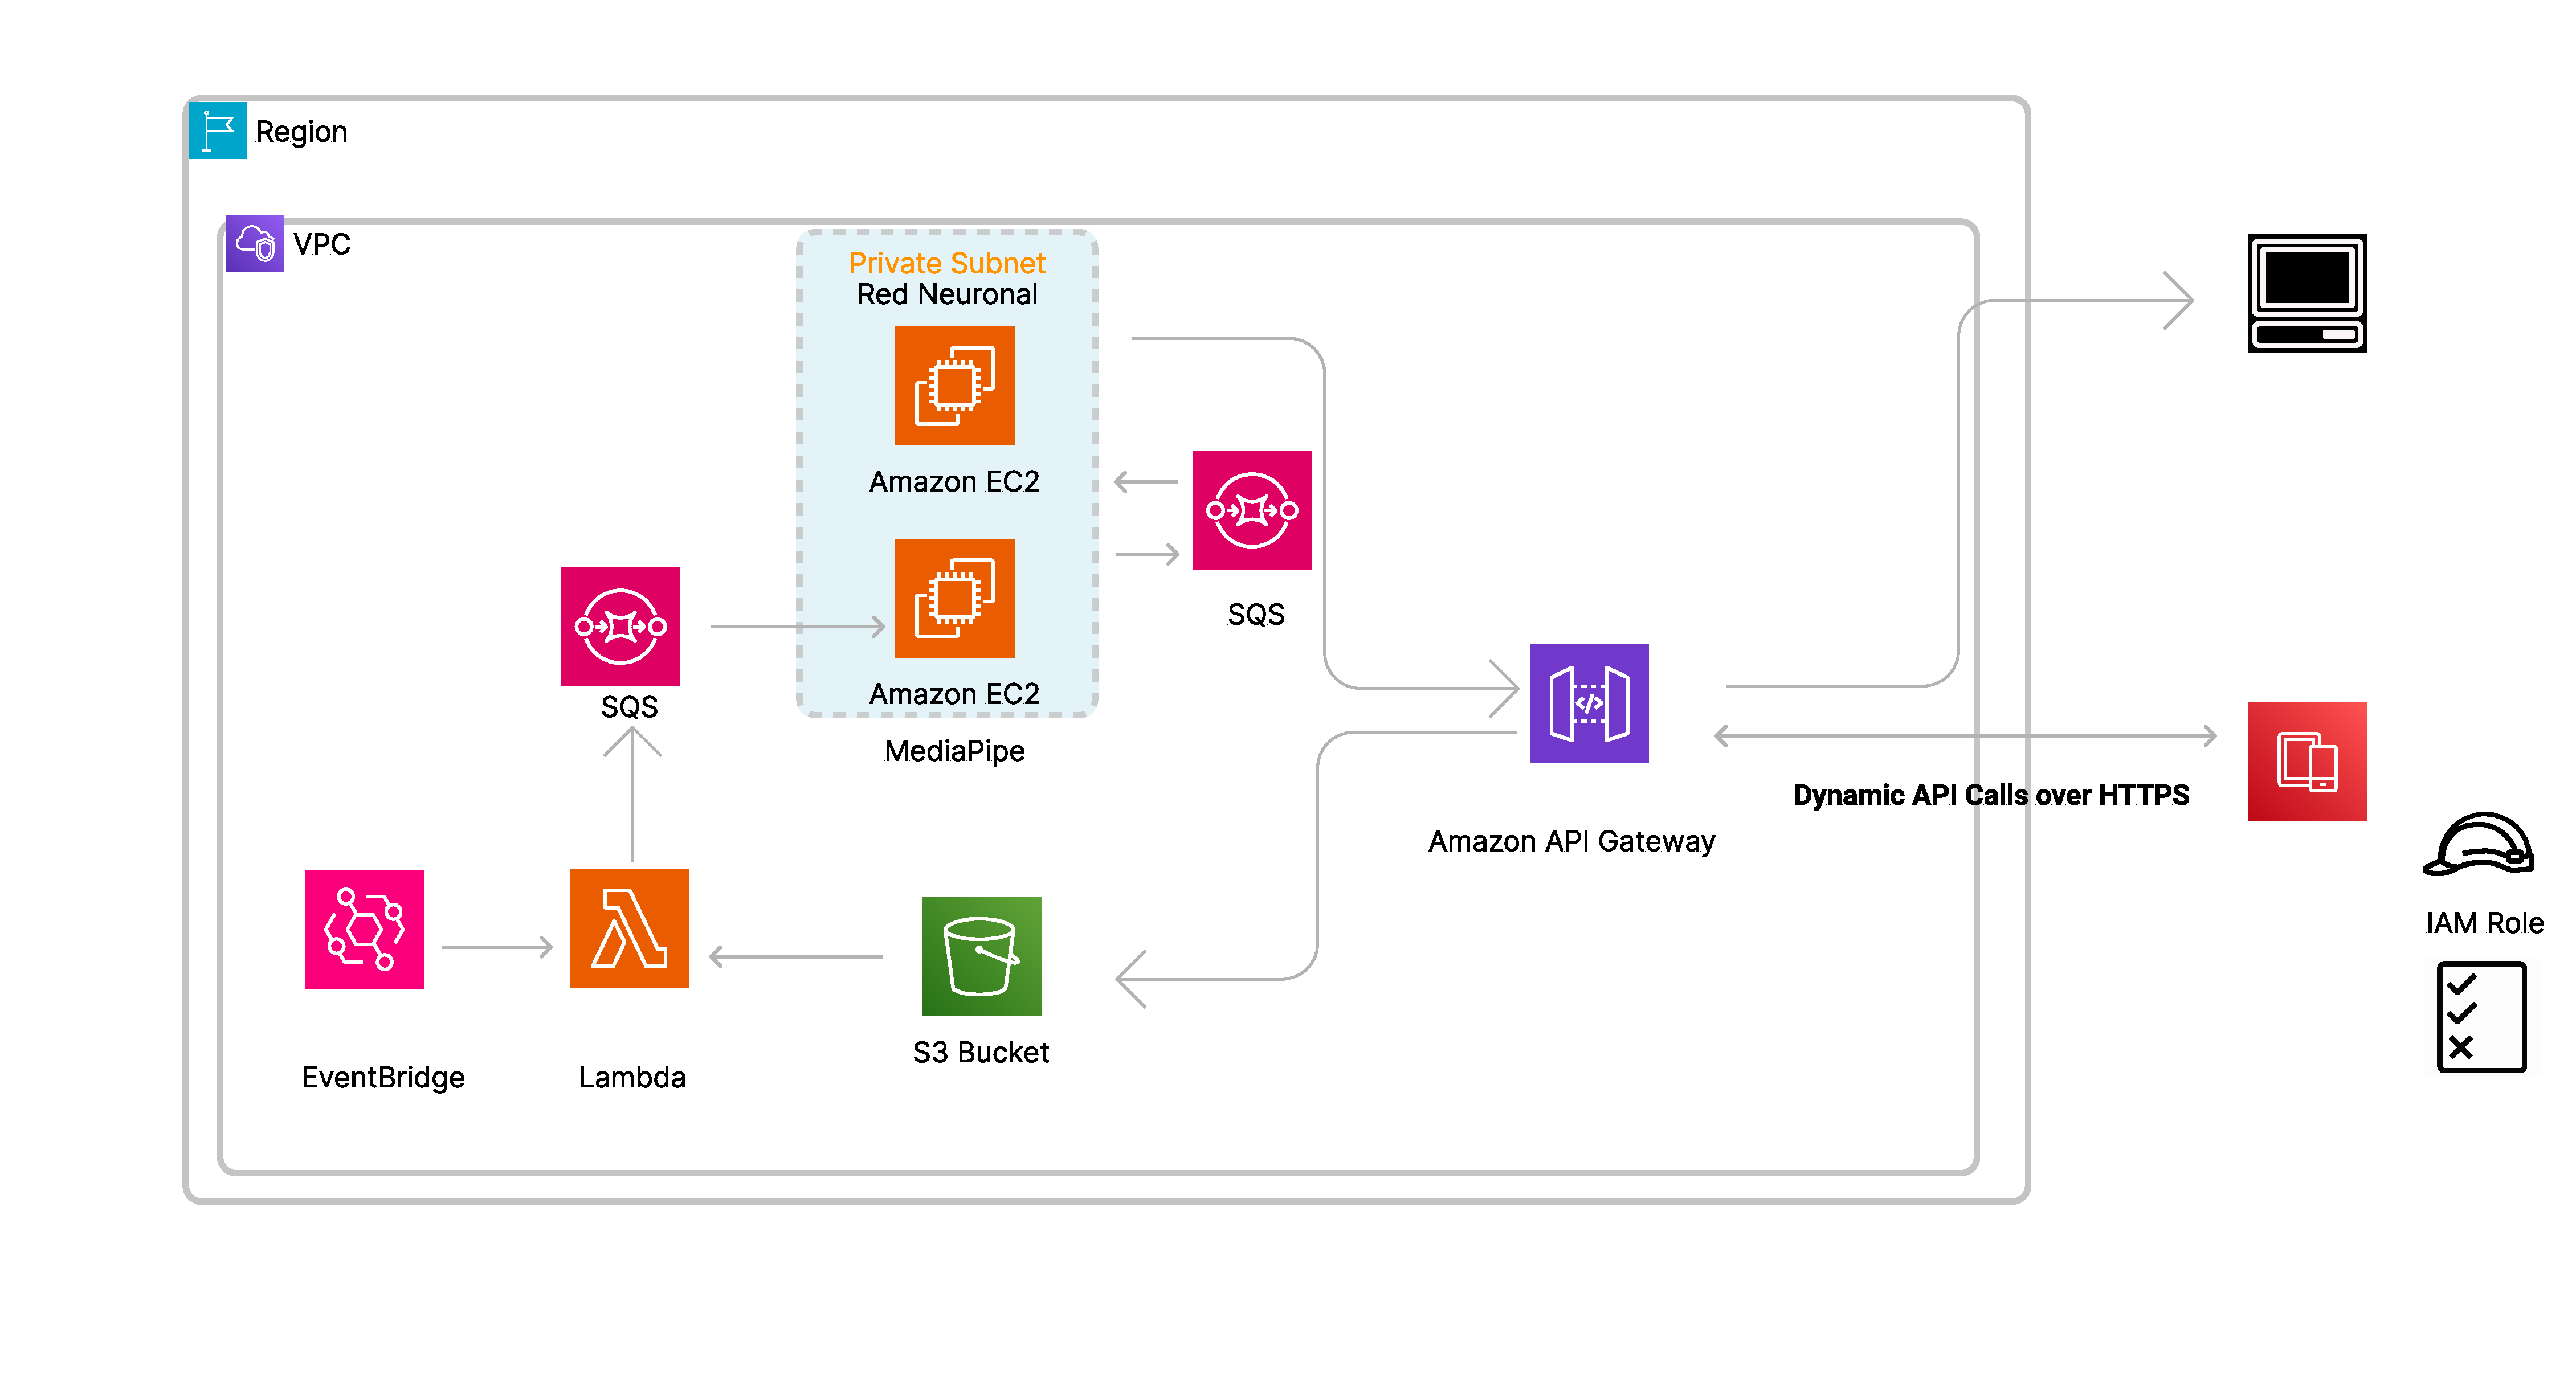
\includegraphics[width=\textwidth]{CAPITULOS/capitulo5/Untitled} % No se incluye la extensión .pdf
\caption{Diagrama de componentes del sistema.}
\label{fig:diagrama_componentes}
\end{figure}
\section{Arquitectura del Sistema}

\begin{itemize}
    \item El programa de obtención de muestreo residirá en un entorno on-premise (en el dispositivo del usuario). Se encargará de capturar los datos, realizar un preprocesamiento básico y enviarlos a la nube.
    \item El sistema de almacenamiento de fotogramas, el entrenamiento del modelo y el despliegue del algoritmo de clasificación se llevarán a cabo en la nube, lo que permitirá escalabilidad y automatización de procesos.
    \item La decisión de desplegar el sistema de traducción en la nube o en un entorno on-premise se basará en un análisis de varios factores, como costo y latencia.
\end{itemize}

\section{Tecnologías Utilizadas}

\begin{itemize}
    \item MediaPipe Holistic (o API similar): Captura y procesamiento de datos de la cámara.
    \item TensorFlow: Entrenamiento y despliegue del modelo de aprendizaje profundo.
    \item Amazon S3: Almacenamiento de fotogramas y datos en la nube.
    \item Python: Lenguaje de programación principal.
    \item API de Text-To-Speech: Generación de mensajes de voz.
    \item Microservicios, SQS, Lambda, EventBridge: Componentes para la arquitectura en la nube (si se opta por esa opción).
    \item Tecnologías web: Sistema web (en conjunto con su framework).
\end{itemize}

\section{Desarrollo de un Sistema de Reconocimiento de Señas}
El sistema de reconocimiento de señas que se desarrollará utilizará principalmente la información de la posición de las falanges de la mano y el antebrazo, capturada a través de una cámara web. Para el seguimiento de manos, se empleará \textbf{MediaPipe Holistic} u otra API de \textbf{hand tracking} que cumpla con criterios de precisión, velocidad, facilidad de integración y soporte para el reconocimiento de la \textbf{Lengua de Señas Mexicana (LSM)}.

Este trabajo se centra en la configuración manual, es decir, en la forma y posición de las manos y los antebrazos durante la realización de una seña. Es importante tener en cuenta que el uso de una cámara implica limitaciones en el campo de visión. Aunque ofrece mayor flexibilidad que algunos sensores, factores como el entorno y la distancia a la cámara pueden afectar la calidad de la captura de datos. Por ello, el sistema se enfocará en la parte superior del cuerpo del usuario, desde los antebrazos hacia arriba, incluyendo las manos, que son las áreas clave para la expresión en LSM.

El flujo de trabajo del sistema, ilustrado en el diagrama \ref{fig:diagrama_composicion}, se desarrolla de la siguiente manera:

\begin{itemize}
    \item \textbf{Iniciar Grabación/Toma de Fotos}: El usuario inicia el proceso, lo que activa la captura de video o fotos.
    \item \textbf{Captura y Procesamiento de Datos}: El sistema divide el video en frames y almacena estos datos localmente antes de subirlos a la nube.
    \item \textbf{Almacenamiento y Notificación}: Los frames se almacenan en un bucket de S3, y se envían notificaciones a través de \textbf{EventBridge}.
    \item \textbf{Invocación de Microservicios}: Se invoca un microservicio que procesa los frames utilizando \textbf{MediaPipe} para extraer características relevantes de las manos y antebrazos.
    \item \textbf{Entrenamiento y Predicción}: Los modelos de machine learning se entrenan con los datos procesados. Cuando el usuario inicia la traducción, el sistema captura frames, predice las palabras en base a un modelo local y genera el audio correspondiente a la seña.
\end{itemize}

El sistema no solo busca reconocer las señas de manera precisa, sino también facilitar la comunicación efectiva mediante la generación de audio en tiempo real, que se reproducirá para el usuario. Además, el enfoque en la parte superior del cuerpo garantiza que se capture adecuadamente la expresión manual esencial para el reconocimiento de la LSM.


\begin{figure}[h]
    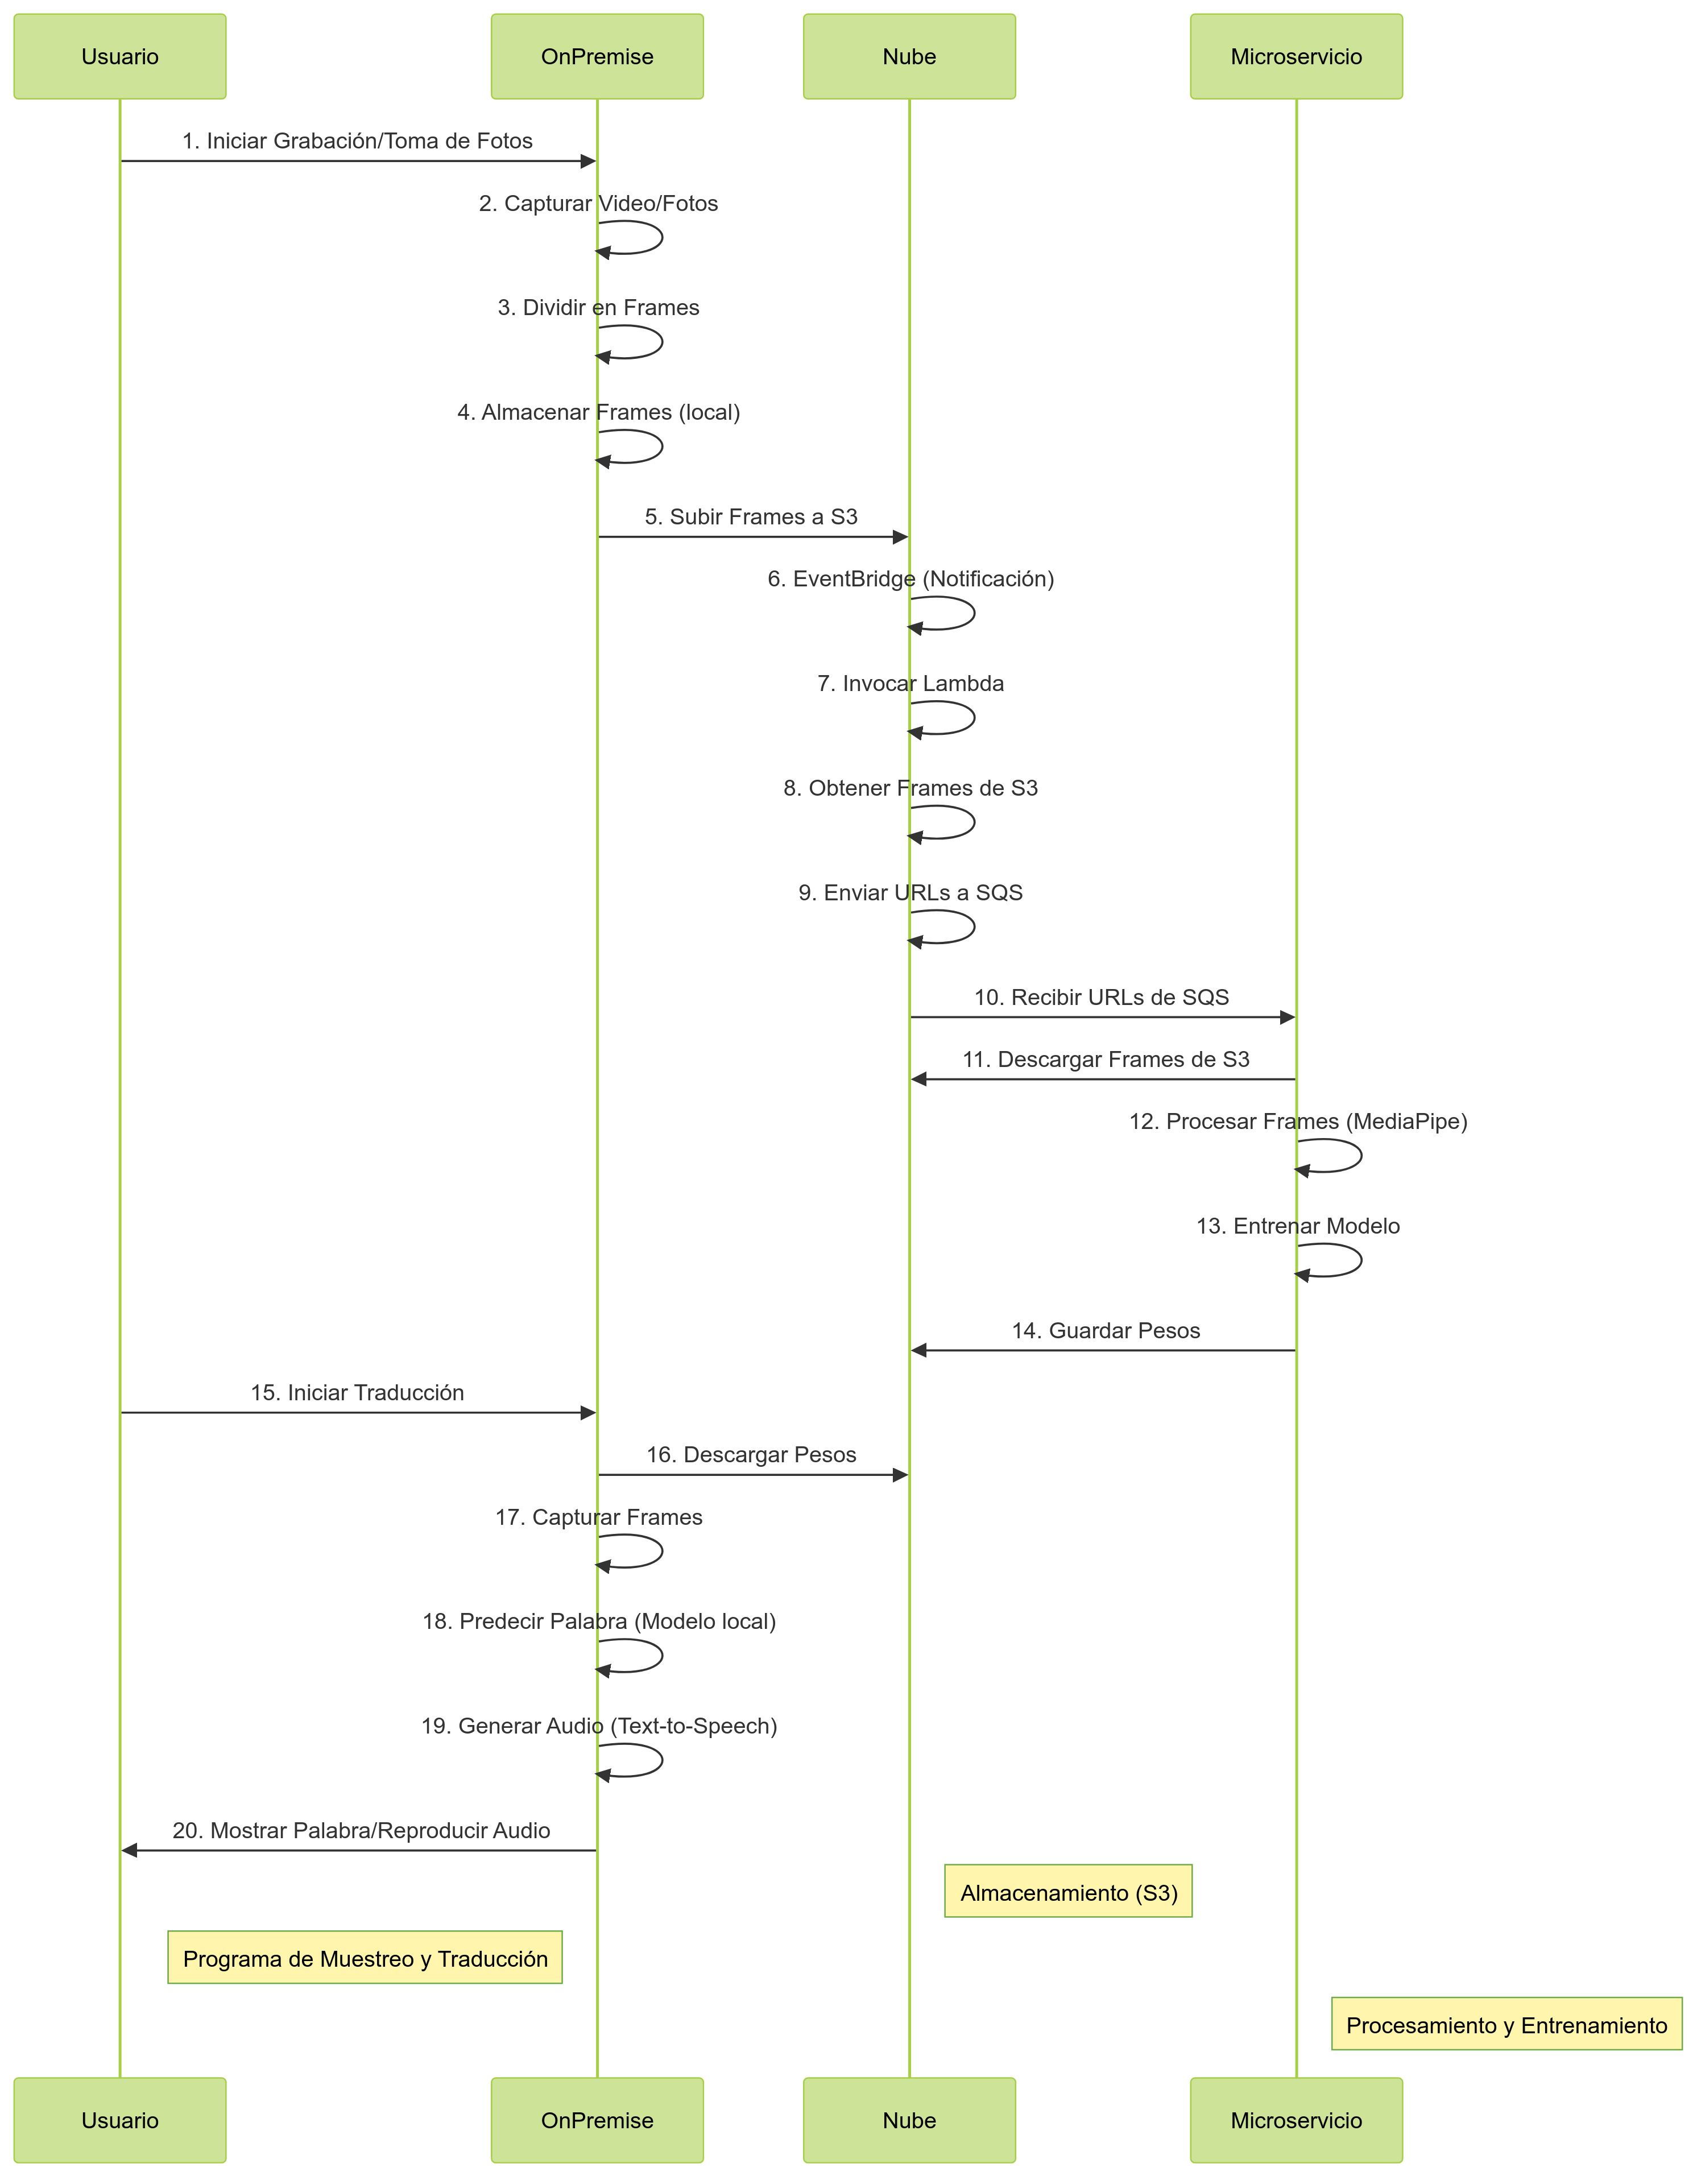
\includegraphics[scale=0.17]{CAPITULOS/capitulo1/segundo.png}
    \centering
    \caption[Diagrama de secuencia composición del sistema ]{Diagrama de secuencia composición del sistema}
    \label{fig:diagrama_composicion}
\end{figure}

\clearpage
\section{Proceso de Muestreo}

El proceso de reconocimiento comenzará cuando el usuario realice un gesto específico de inicio, como alzar la mano. A partir de ese momento, se capturarán fotogramas (frames) de la seña. Estos datos se almacenarán en la nube, utilizando un servicio como Amazon S3, para su posterior procesamiento.

\section{Proceso de Extracción de Datos y Entrenamiento}

La API de MediaPipe Holistic (u otra similar) se encargará de procesar los fotogramas y extraer la posición de los puntos de referencia relevantes en las manos y antebrazos. Una vez que se hayan recopilado suficientes muestras de entrenamiento, se utilizará un microservicio en Python que utilice TensorFlow o Keras para entrenar un modelo de aprendizaje profundo capaz de reconocer las señas. Este modelo se desplegará en la nube para garantizar la escalabilidad y el manejo eficiente de las solicitudes de entrenamiento.

\section{Reconocimiento y Traducción de Señas}

El algoritmo entrenado clasificará la seña emitida, comparándola con las señas previamente clasificadas y entradas. Para ello, utilizará la información de la posición de los puntos de referencia proporcionada por la API de hand tracking y realizará un mapeo a la configuración manual de la seña, como entrada al modelo. Una vez que se logre el reconocimiento de una seña dentro de la LSM, el sistema proporcionará la traducción al español, seguida de un mensaje de voz generado mediante una API de Text-To-Speech.



\section{Base de datos}
\label{sec:base_datos}


Para este módulo se decidió utilizar una base de datos documental (NoSQL).

\subsection{Estructura de las colecciones de Firebase}

A continuación se muestra la estructura de las colecciones de Firebase:

\subsection{Colección usuarios}

\begin{lstlisting}[style=json, caption=Documento de ejemplo en la colección 'usuarios', label=lst:usuarios]
{
  "uid1": {
    "nombre": "jose daniel alvarez ramos",
    "correo": "jalvarezr1001@alumno.ipn.mx",
    "rolId": "admin", // Referencia al documento 'admin' de 'roles'
    "fechaCreacion": "2024-11-09T12:00:00Z",
    "ultimaModificacion": "2024-11-09T12:00:00Z",
    "activo": true,
    "destacados": {
      "conteo": 10,
      "fechaCreacion": "2024-11-09T12:00:00Z",
      "ultimaModificacion": "2024-11-09T12:00:00Z",
      "activo": true
    }
  },
  "uid2": {
    // ... otros usuarios
  }
}
\end{lstlisting}

\subsection{Colección señas}

\begin{lstlisting}[style=json, caption=Documento de ejemplo en la colección 'senas', label=lst:senas]
{
  "sena": {
    "nombre": "Hola",
    "descripcion": "Descripción de la Seña "hola"",
    "videoUrl": "https://bucket.com/hola.mp4",
    "usuarioId": "uid1", // Referencia al documento 'uid1' de 'usuarios'
    "fechaCreacion": "2024-11-09T12:00:00Z",
    "ultimaModificacion": "2024-11-09T12:00:00Z",
    "activo": true
  },
  "sena": {
    // ... otras senas
  }
}
\end{lstlisting}

\subsection{Colección roles}

\begin{lstlisting}[style=json, caption=Documento de ejemplo en la colección 'roles', label=lst:roles]
{
  "admin": {
    "nombre": "Administrador",
    "activo": true
  },
  "usuario": {
    // ... otros roles
  }
}
\end{lstlisting}

\section{Diccionario LSM}
\label{sec:diccionario_LSM}

El \textbf{Diccionario LSM} es un recurso clave en el sistema de traducción, diseñado para almacenar y organizar un extenso repertorio de señas en Lengua de Señas Mexicana (LSM). Este diccionario proporciona las referencias necesarias para el reconocimiento y la correcta traducción de señas, facilitando tanto el aprendizaje de LSM como la interacción entre personas oyentes y personas sordas.

\subsection{Señas y Descripciones}

\begin{itemize}
        % Seña "Bien" con 4 fotogramas
    \item \textbf{Seña: Bien} \\
    La figura a continuación muestra diferentes perspectivas para realizar la seña ``Bien'' en LSM.
    \begin{figure}[H]
        \centering
        \begin{minipage}{0.42\textwidth}
            \centering
            \subfloat[1]{%
                \includegraphics[page=1, width=\textwidth]{CAPITULOS/capitulo5/bien.pdf}
            }
        \end{minipage}%
        \hspace{0.05\textwidth}
        \begin{minipage}{0.42\textwidth}
            \centering
            \subfloat[2]{%
                \includegraphics[page=2, width=\textwidth]{CAPITULOS/capitulo5/bien.pdf}
            }
        \end{minipage}

        \vspace{10pt}

        \begin{minipage}{0.42\textwidth}
            \centering
            \subfloat[3]{%
                \includegraphics[page=3, width=\textwidth]{CAPITULOS/capitulo5/bien.pdf}
            }
        \end{minipage}%
        \hspace{0.05\textwidth}
        \begin{minipage}{0.42\textwidth}
            \centering
            \subfloat[4]{%
                \includegraphics[page=4, width=\textwidth]{CAPITULOS/capitulo5/bien.pdf}
            }
        \end{minipage}

        \caption{Composición de la Seña ``Bien'' en LSM}
        \label{fig:seña_bien}
    \end{figure}

    % Seña "Hola" con 3 fotogramas
    \item \textbf{Seña: Hola} \\
    \begin{figure}[H]
        \centering
        \begin{minipage}{0.42\textwidth}
            \centering
            \subfloat[1]{%
                \includegraphics[page=1, width=\textwidth]{CAPITULOS/capitulo5/hola.pdf}
            }
        \end{minipage}%
        \hspace{0.05\textwidth}
        \begin{minipage}{0.42\textwidth}
            \centering
            \subfloat[2]{%
                \includegraphics[page=2, width=\textwidth]{CAPITULOS/capitulo5/hola.pdf}
            }
        \end{minipage}

        \vspace{10pt}

        \begin{minipage}{0.45\textwidth}
            \centering
            \subfloat[3]{%
                \includegraphics[page=3, width=\textwidth]{CAPITULOS/capitulo5/hola.pdf}
            }
        \end{minipage}

        \caption{Composición de la Seña ``Hola'' en LSM}
        \label{fig:seña_hola}
    \end{figure}

    % Seña "Mal" con 4 fotogramas
    \item \textbf{Seña: Mal} \\
    \begin{figure}[H]
        \centering
        \begin{minipage}{0.42\textwidth}
            \centering
            \subfloat[1]{%
                \includegraphics[page=1, width=\textwidth]{CAPITULOS/capitulo5/mal.pdf}
            }
        \end{minipage}%
        \hspace{0.05\textwidth}
        \begin{minipage}{0.42\textwidth}
            \centering
            \subfloat[2]{%
                \includegraphics[page=2, width=\textwidth]{CAPITULOS/capitulo5/mal.pdf}
            }
        \end{minipage}

        \vspace{10pt}

        \begin{minipage}{0.45\textwidth}
            \centering
            \subfloat[3]{%
                \includegraphics[page=3, width=\textwidth]{CAPITULOS/capitulo5/mal.pdf}
            }
        \end{minipage}%
        \hspace{0.05\textwidth}
        \begin{minipage}{0.45\textwidth}
            \centering
            \subfloat[4]{%
                \includegraphics[page=4, width=\textwidth]{CAPITULOS/capitulo5/mal.pdf}
            }
        \end{minipage}

        \caption{Composición de la Seña ``Mal'' en LSM}
        \label{fig:seña_mal}
    \end{figure}

    % Seña "¿Cómo estás?" con 5 fotogramas
    \item \textbf{Seña: ¿Cómo estás?} \\
    \begin{figure}[H]
        \centering
        \begin{minipage}{0.28\textwidth}
            \centering
            \subfloat[1]{%
                \includegraphics[page=1, width=\textwidth]{CAPITULOS/capitulo5/como.pdf}
            }
        \end{minipage}%
        \hspace{0.05\textwidth}
        \begin{minipage}{0.28\textwidth}
            \centering
            \subfloat[2]{%
                \includegraphics[page=2, width=\textwidth]{CAPITULOS/capitulo5/como.pdf}
            }
        \end{minipage}

        \vspace{10pt}

        \begin{minipage}{0.28\textwidth}
            \centering
            \subfloat[3]{%
                \includegraphics[page=3, width=\textwidth]{CAPITULOS/capitulo5/como.pdf}
            }
        \end{minipage}%
        \hspace{0.05\textwidth}
        \begin{minipage}{0.28\textwidth}
            \centering
            \subfloat[4]{%
                \includegraphics[page=4, width=\textwidth]{CAPITULOS/capitulo5/como.pdf}
            }
        \end{minipage}

        \vspace{10pt}

        \begin{minipage}{0.3\textwidth}
            \centering
            \subfloat[5]{%
                \includegraphics[page=5, width=\textwidth]{CAPITULOS/capitulo5/como.pdf}
            }
        \end{minipage}

        \caption{Composición de la Seña ``¿Cómo estás?'' en LSM}
        \label{fig:seña_como_estas}
    \end{figure}

    \item \textbf{Seña: Doctor} \\
    \begin{figure}[H]
        \centering
        \begin{minipage}{0.42\textwidth}
            \centering
            \subfloat[1]{%
                \includegraphics[page=1, width=\textwidth]{CAPITULOS/capitulo5/doctor}
            }
        \end{minipage}%
        \hspace{0.05\textwidth}
        \begin{minipage}{0.42\textwidth}
            \centering
            \subfloat[2]{%
                \includegraphics[page=2, width=\textwidth]{CAPITULOS/capitulo5/doctor}
            }
        \end{minipage}

        \vspace{10pt}

        \begin{minipage}{0.45\textwidth}
            \centering
            \subfloat[3]{%
                \includegraphics[page=3, width=\textwidth]{CAPITULOS/capitulo5/doctor}
            }
        \end{minipage}

        \caption{Composición de la Seña ``Doctor'' en LSM}
        \label{fig:seña_doctor}
    \end{figure}

    % Seña "Mal" con 4 fotogramas
    \item \textbf{Seña: Emergencia} \\
    \begin{figure}[H]
        \centering
        \begin{minipage}{0.42\textwidth}
            \centering
            \subfloat[1]{%
                \includegraphics[page=1, width=\textwidth]{CAPITULOS/capitulo5/emergencia}
            }
        \end{minipage}%
        \hspace{0.05\textwidth}
        \begin{minipage}{0.42\textwidth}
            \centering
            \subfloat[2]{%
                \includegraphics[page=2, width=\textwidth]{CAPITULOS/capitulo5/emergencia}
            }
        \end{minipage}

        \vspace{10pt}

        \begin{minipage}{0.45\textwidth}
            \centering
            \subfloat[3]{%
                \includegraphics[page=3, width=\textwidth]{CAPITULOS/capitulo5/emergencia}
            }
        \end{minipage}%
        \hspace{0.05\textwidth}
        \begin{minipage}{0.45\textwidth}
            \centering
            \subfloat[4]{%
                \includegraphics[page=4, width=\textwidth]{CAPITULOS/capitulo5/emergencia}
            }
        \end{minipage}

        \caption{Composición de la Seña ``Emergencia'' en LSM}
        \label{fig:seña_emergencia}
    \end{figure}

    % Seña "Hola" con 3 fotogramas
    \item \textbf{Seña: Por favor} \\
    \begin{figure}[H]
        \centering
        \begin{minipage}{0.42\textwidth}
            \centering
            \subfloat[1]{%
                \includegraphics[page=1, width=\textwidth]{CAPITULOS/capitulo5/porfavor}
            }
        \end{minipage}%
        \hspace{0.05\textwidth}
        \begin{minipage}{0.42\textwidth}
            \centering
            \subfloat[2]{%
                \includegraphics[page=2, width=\textwidth]{CAPITULOS/capitulo5/porfavor}
            }
        \end{minipage}

        \vspace{10pt}

        \begin{minipage}{0.45\textwidth}
            \centering
            \subfloat[3]{%
                \includegraphics[page=3, width=\textwidth]{CAPITULOS/capitulo5/porfavor}
            }
        \end{minipage}

        \caption{Composición de la Seña ``Por favor'' en LSM}
        \label{fig:seña_porfavor}
    \end{figure}

    % Seña "Mal" con 4 fotogramas
    \item \textbf{Seña: Síntoma} \\
    \begin{figure}[H]
        \centering
        \begin{minipage}{0.42\textwidth}
            \centering
            \subfloat[1]{%
                \includegraphics[page=1, width=\textwidth]{CAPITULOS/capitulo5/sintoma}
            }
        \end{minipage}%
        \hspace{0.05\textwidth}
        \begin{minipage}{0.42\textwidth}
            \centering
            \subfloat[2]{%
                \includegraphics[page=2, width=\textwidth]{CAPITULOS/capitulo5/sintoma}
            }
        \end{minipage}

        \vspace{10pt}

        \begin{minipage}{0.45\textwidth}
            \centering
            \subfloat[3]{%
                \includegraphics[page=3, width=\textwidth]{CAPITULOS/capitulo5/sintoma}
            }
        \end{minipage}%
        \hspace{0.05\textwidth}
        \begin{minipage}{0.45\textwidth}
            \centering
            \subfloat[4]{%
                \includegraphics[page=4, width=\textwidth]{CAPITULOS/capitulo5/sintoma}
            }
        \end{minipage}

        \caption{Composición de la Seña ``Síntoma'' en LSM}
        \label{fig:seña_sintoma}
    \end{figure}

    \item \textbf{Seña: Temperatura} \\
    \begin{figure}[H]
        \centering
        \begin{minipage}{0.42\textwidth}
            \centering
            \subfloat[1]{%
                \includegraphics[page=1, width=\textwidth]{CAPITULOS/capitulo5/temperatura}
            }
        \end{minipage}%
        \hspace{0.05\textwidth}
        \begin{minipage}{0.42\textwidth}
            \centering
            \subfloat[2]{%
                \includegraphics[page=2, width=\textwidth]{CAPITULOS/capitulo5/temperatura}
            }
        \end{minipage}

        \vspace{10pt}

        \begin{minipage}{0.45\textwidth}
            \centering
            \subfloat[3]{%
                \includegraphics[page=3, width=\textwidth]{CAPITULOS/capitulo5/temperatura}
            }
        \end{minipage}%
        \hspace{0.05\textwidth}
        \begin{minipage}{0.45\textwidth}
            \centering
            \subfloat[4]{%
                \includegraphics[page=4, width=\textwidth]{CAPITULOS/capitulo5/temperatura}
            }
        \end{minipage}

        \caption{Composición de la Seña ``Temperatura'' en LSM}
        \label{fig:seña_temperatura}
    \end{figure}

    \item \textbf{Seña: Enfermo} \\
    \begin{figure}[H]
        \centering
        \begin{minipage}{0.42\textwidth}
            \centering
            \subfloat[1]{%
                \includegraphics[page=1, width=\textwidth]{CAPITULOS/capitulo5/enfermo}
            }
        \end{minipage}%
        \hspace{0.05\textwidth}
        \begin{minipage}{0.42\textwidth}
            \centering
            \subfloat[2]{%
                \includegraphics[page=2, width=\textwidth]{CAPITULOS/capitulo5/enfermo}
            }
        \end{minipage}

        \vspace{10pt}

        \begin{minipage}{0.45\textwidth}
            \centering
            \subfloat[3]{%
                \includegraphics[page=3, width=\textwidth]{CAPITULOS/capitulo5/enfermo}
            }
        \end{minipage}%
        \hspace{0.05\textwidth}
        \begin{minipage}{0.45\textwidth}
            \centering
            \subfloat[4]{%
                \includegraphics[page=4, width=\textwidth]{CAPITULOS/capitulo5/enfermo}
            }
        \end{minipage}

        \caption{Composición de la Seña ``Enfermo'' en LSM}
        \label{fig:seña_enfermo}
    \end{figure}
\end{itemize}

\section{Interfaz de usuario de la aplicación}

La aplicación móvil se ha diseñado con una interfaz intuitiva y fácil de usar, con el objetivo de proporcionar una experiencia de usuario fluida y accesible. A continuación, se describen las principales pantallas de la aplicación, diferenciando entre los roles de usuario (administrador y general) cuando sea necesario:

\subsection{Splash Screen}

\begin{figure}[h]
    \centering
    \fbox{\includegraphics[page=1, scale=0.5]{CAPITULOS/capitulo5/proyecto}}
    \caption{Splash Screen de la aplicación.}
\end{figure}

Esta es la primera pantalla que se muestra al iniciar la aplicación. Su función principal es mostrar el ícono de la aplicación mientras se cargan los componentes necesarios.  Es visible tanto para usuarios administradores como generales.

\subsection{Login}

\begin{figure}[h]
    \centering
    \fbox{\includegraphics[page=2, scale=0.5]{CAPITULOS/capitulo5/proyecto}}
    \caption{Pantalla de inicio de sesión.}
\end{figure}

Esta pantalla permite a todos los usuarios iniciar sesión en la aplicación. Se requiere una dirección de correo electrónico y una contraseña para la autenticación, la cual se gestiona a través de Firebase.

\subsubsection{Funcionalidad}

\begin{itemize}
    \item \textbf{Inicio de sesión con correo electrónico y contraseña:} Disponible para todos los usuarios.
    \item \textbf{Inicio de sesión con Google:} Disponible solo para usuarios con rol general.
    \item \textbf{Registro de nuevo usuario:} Permite a los usuarios que no están registrados crear una cuenta utilizando su correo electrónico y contraseña, o a través de su cuenta de Google.
\end{itemize}
\subsection{Pantalla principal (Usuario general)}

\begin{figure}[h]
    \centering
    \fbox{\includegraphics[page=3, scale=0.5]{CAPITULOS/capitulo5/proyecto}}
    \caption{Pantalla principal para usuarios con rol general.}
\end{figure}

Esta es la pantalla principal a la que acceden los usuarios con rol general después de iniciar sesión.

\subsubsection{Diseño}

El diseño de la pantalla principal es simple y directo. En la parte superior se encuentra el logo de la aplicación, y en la parte central se muestran las opciones principales, como "Traducir" y "Diccionario". Cada opción se representa con un icono y un texto descriptivo.

\subsubsection{Funcionalidad}

Al tocar una de las opciones, el usuario es redirigido a la pantalla correspondiente. Por ejemplo, al tocar "Traducir", se abre la pantalla de traducción en tiempo real.

\subsection{Pantalla principal (Usuario administrador)}

\begin{figure}[h]
    \centering
    \fbox{\includegraphics[page=4, scale=0.5]{CAPITULOS/capitulo5/proyecto}}
    \caption{Pantalla principal para usuarios administradores.}
\end{figure}

Esta es la pantalla principal a la que acceden los usuarios administradores después de iniciar sesión.

[Aquí deberías describir el diseño y la funcionalidad específica de la pantalla principal para el usuario administrador, incluyendo las opciones adicionales a las que tiene acceso, como la gestión de usuarios, la edición del diccionario, etc.]

\subsection{Pantalla del diccionario}

\begin{figure}[h]
    \centering
    \fbox{\includegraphics[page=5, scale=0.5]{CAPITULOS/capitulo5/proyecto}}
    \caption{Pantalla del diccionario LSM.}
\end{figure}

[El resto de la descripción de la pantalla del diccionario se mantiene igual]




% Añadir bibliografía
    \printbibliography

\end{document}